\documentclass[a4paper,12pt]{article}
\usepackage{fontspec}
\usepackage{xeCJK}
\setmainfont{Times New Roman}
\usepackage{amsmath}
\usepackage{amsthm}
\usepackage{amsfonts}
\usepackage{amssymb}
\usepackage{graphicx}
\usepackage{hyperref}
\usepackage{enumitem}
\usepackage{textcomp}
\usepackage{float}
\usepackage{booktabs}
\usepackage{url}
\usepackage[colorinlistoftodos]{todonotes}
\usepackage[left=1.50cm, right=1.50cm, top=1.20cm]{geometry}
\linespread{1.5}
\usepackage{algorithm}
\usepackage{algpseudocode}
\usepackage{tikz}
\usepackage[tikz]{mdframed}
\usetikzlibrary{matrix, positioning, fit, arrows, calc, intersections, shapes, shadings, patterns, decorations.markings, chains, scopes, shapes.arrows}
\usepackage{upquote}
\usepackage{tikzpeople}
\usepackage{tikzsymbols}
\usepackage{listings}
\usepackage{color}
\usepackage{logicpuzzle}
\usepackage{subcaption}
\usepackage[tikz]{mdframed}
\lstdefinestyle{customc}{
  belowcaptionskip=1\baselineskip,
  breaklines=true,
  frame=L,
  xleftmargin=\parindent,
  language=C++,
  tabsize=2,
  %numbers=left,
  %stepnumber=1,
  showstringspaces=false,
  basicstyle=\small\ttfamily,
  keywordstyle=\bfseries\color{green!40!black},
  commentstyle=\itshape\color{purple!40!black},
  identifierstyle=\color{blue},
  stringstyle=\color{orange},
}
\mdfdefinestyle{mymdf}{leftmargin=1cm,rightmargin=2cm,%
innerleftmargin=1cm,innerrightmargin=1cm,roundcorner=10pt,backgroundcolor=lg}
\definecolor{lg}{RGB}{247,249,250}
\title{Algorithm Problem Set \\ \large No. 700 --- 799}
\author{SS}
\date{July 2019}

\begin{document}
\renewcommand{\thelstlisting}{\thesection.\arabic{lstlisting}}
\newcommand{\fcc}[1]{\lstinline[language=C++, basicstyle=\small\ttfamily, keywordstyle=\bfseries\color{green!40!black}]|#1|}
\newcommand{\fcj}[1]{\lstinline[language=Java, basicstyle=\small\ttfamily, keywordstyle=\bfseries\color{green!40!black}]|#1|}
%\sloppy
\maketitle
\section{701 --- Insert into a Binary Search Tree}
Given the root node of a binary search tree (BST) and a value to be inserted into the tree, insert the value into the BST. Return the root node of the BST after the insertion. It is guaranteed that the new value does not exist in the original BST.

Note that there may exist multiple valid ways for the insertion, as long as the tree remains a BST after insertion. You can return any of them.

For example, 

Given the tree:

\begin{figure}[H]
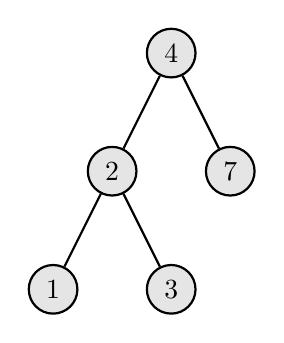
\begin{tikzpicture}
[every node/.style={draw, circle, fill=gray!20!, minimum size=5mm}, 
thick]
\node{4}
child{node{2} child{node{1}} child{node{3}}}
child{node{7}};
\end{tikzpicture}
\end{figure}

And the value to insert: 5

You can return this binary search tree:

\begin{figure}[H]
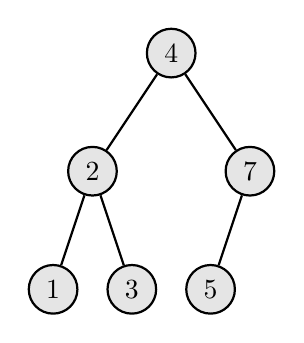
\begin{tikzpicture}
[every node/.style={draw, circle, fill=gray!20!, minimum size=5mm}, 
level 1/.style={sibling distance=20mm},
level 2/.style={sibling distance=10mm},
thick]
\node{4}
child{node{2} child{node{1}} child{node{3}}}
child{node{7} child{node{5}} child[missing]};
\end{tikzpicture}
\end{figure}

This tree is also valid:

\begin{figure}[H]
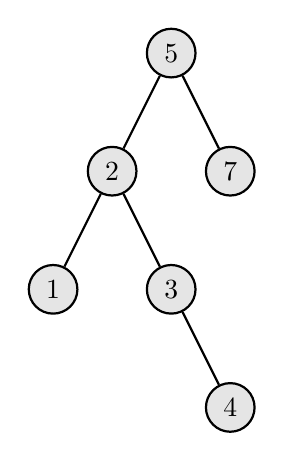
\begin{tikzpicture}
[every node/.style={draw, circle, fill=gray!20!, minimum size=5mm},
thick]
\node{5}
child{node{2} child{node{1}} child{node{3} child[missing] child{node{4}}}}
child{node{7}};
\end{tikzpicture}
\end{figure}

\subsection{Recursion}
Notice this is insertion not deletion. 

So, the approach is simple we can always insert new node as a child of the leaf. To define which leaf to use, we follow the standard BST logic :


\begin{itemize}
\item If \fcj{val > node.val}, go to insert into the right subtree.
\item If \fcj{val < node.val}, go to insert into the left subtree.
\end{itemize}

\setcounter{lstlisting}{0}
\begin{lstlisting}[style=customc, caption={Recursion}]
TreeNode* insertIntoBST( TreeNode* root, int val )
{
    if( !root )
    {
        return new TreeNode( val );
    }

    if( val < root->val )
    {
		//insert into left child
        root->left = insertIntoBST( root->left, val );
    }
    else
    {
		//insert into right child
        root->right = insertIntoBST( root->right, val );
    }

    return root;
}
\end{lstlisting}




\section{702 --- Search in a Sorted Array of Unknown Size}
Given an integer array sorted in ascending order, write a function to search \textbf{target} in nums.  If \textbf{target} exists, then return its index, otherwise return $-1$. However, the array size is unknown to you. You may only access the array using an \fcj{ArrayReader} interface, where \fcj{ArrayReader.get(k)} returns the element of the array at index $k$ (0-indexed).

You may assume all integers in the array are less than 10000, and if you access the array out of bounds, \fcj{ArrayReader.get} will return 2147483647.

\paragraph{Example 1:}

\begin{flushleft}
\textbf{Input}: \fcj{array = [-1,0,3,5,9,12], target = 9}

\textbf{Output}: 4

\textbf{Explanation}: 9 exists and its index is 4
\end{flushleft}

\paragraph{Example 2:}

\begin{flushleft}
\textbf{Input}: \fcj{array = [-1,0,3,5,9,12], target = 2}

\textbf{Output}: $-1$

\textbf{Explanation}: 2 does not exist so return $-1$
\end{flushleft}

 

\paragraph{Note:}

\begin{itemize}
\item You may assume that all elements in the array are unique.
\item The value of each element in the array will be in the range \fcj{[-9999, 9999]}.
\end{itemize}

\subsection{Binary Search}
Since array is sorted, binary search is one of feasible approach, but the problem here is that we don’t know size of array.

If the array size is unknown, that means we do not have proper bounds to apply binary search. So in order to find position of key, first we find bounds and then apply binary search algorithm.
\begin{itemize}
    \item Let $l$ be pointing to 1st element and $h$ pointing to 2nd element of array, Now compare key with element at index $h$,
    \item if it is greater than the element, set $l\gets h$ and $h\gets h\times 2$.
    \item if it is smaller, then apply binary search on range $(l,h)$.
\end{itemize}

\setcounter{lstlisting}{0}
\begin{lstlisting}[style=customc, caption={Binary Search}]
// Forward declaration of ArrayReader class.
class ArrayReader;

int search( const ArrayReader& reader, int target )
{
    int low = 0;
    int high = 1;

    int x = reader.get( high );

    //find bounds [low, high]
    while( target > x )
    {
        low  = high;
        high *= 2;
        x = reader.get( high );
    }

    int ans = -1;

    //binary search on [low, high]
    while( low <= high )
    {
        int mid = ( low + high ) / 2;

        x = reader.get( mid );

        if( target > x )
        {
            low = mid + 1;
        }
        else if( target < x )
        {
            high = mid - 1;
        }
        else
        {
            ans = mid;
            break;
        }
    }

    return ans;

}
\end{lstlisting}
\section{708 --- Insert into a Cyclic Sorted List}
Given a node from a cyclic linked list which is sorted in ascending order, write a function to insert a value into the list such that it remains a cyclic sorted list. The given node can be a reference to any single node in the list, and may not be necessarily the smallest value in the cyclic list.

If there are multiple suitable places for insertion, you may choose any place to insert the new value. After the insertion, the cyclic list should remain sorted.

If the list is empty (i.e., given node is \fcj{null}), you should create a new single cyclic list and return the reference to that single node. Otherwise, you should return the original given node.

The following example may help you understand the problem better:


\begin{figure}[H]
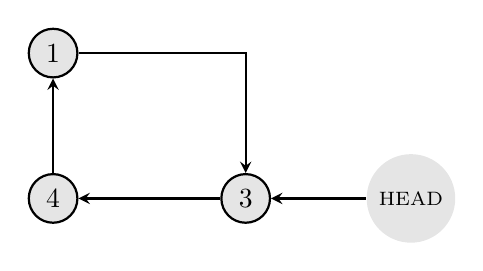
\begin{tikzpicture}
[every node/.style={draw, circle, fill=gray!20!, minimum size=5mm},
>=stealth, ->, thick]
\node(1){1};
\node(4)[below=12mm of 1]{4};
\node(3)[right=18mm of 4]{3};
\draw (4) -- (1);
\draw (1.east) -| (3.north);
\node(t)[draw=none, right=12mm of 3]{\scriptsize HEAD};
\draw (t) -- (3);
\draw (3) -- (4);
\end{tikzpicture}
\end{figure} 



In the figure above, there is a cyclic sorted list of three elements. You are given a reference to the node with value 3, and we need to insert 2 into the list.

 



The new node should insert between node 1 and node 3. After the insertion, the list should look like this, and we should still return node 3.

\begin{figure}[H]
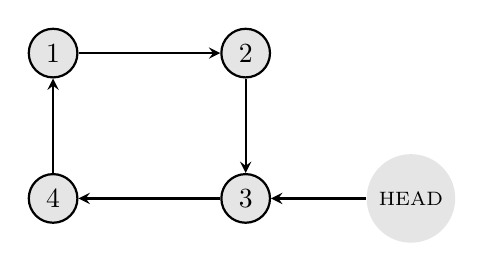
\begin{tikzpicture}
[every node/.style={draw, circle, fill=gray!20!, minimum size=5mm},
>=stealth, ->, thick]
\node(1){1};
\node(2)[right=18mm of 1] {2};
\node(4)[below=12mm of 1]{4};
\node(3)[right=18mm of 4]{3};
\draw (4) -- (1);
\draw (1) -- (2);
\draw (2) -- (3);
\node(t)[draw=none, right=12mm of 3]{\scriptsize HEAD};
\draw (t) -- (3);
\draw (3) -- (4);
\end{tikzpicture}
\end{figure}


% \section{710 --- Random Pick with Blacklist}
Given a blacklist $B$ containing unique integers from $[0, N)$, write a function to return a uniform random integer from $[0, N)$ which is \textbf{NOT} in $B$.

Optimize it such that it minimizes the call to system's \fcj{Math.random()}.

\paragraph{Note:}

\begin{enumerate}
\item $1 \leq N \leq 10^9$
\item $0 \leq \lvert B\rvert < \min(10^5, N)$
\item $[0, N)$ does NOT include $N$. 
\end{enumerate}

\paragraph{Example 1:}

\begin{flushleft}
\textbf{Input}: 

\fcj{["Solution","pick","pick","pick"]}

\fcj{[[1,[]],[],[],[]]}

\textbf{Output}: \fcj{[null,0,0,0]}
\end{flushleft}

\section{Example 2:}

\begin{flushleft}
\textbf{Input}: 

\fcj{["Solution","pick","pick","pick"]}

\fcj{[[2,[]],[],[],[]]}

\textbf{Output}: \fcj{[null,1,1,1]}
\end{flushleft}

\paragraph{Example 3:}

\begin{flushleft}
\textbf{Input}: 
\fcj{["Solution","pick","pick","pick"]}

\fcj{[[3,[1]],[],[],[]]}

\textbf{Output}: \fcj{[null,0,0,2]}
\end{flushleft}

\paragraph{Example 4:}

\begin{flushleft}
\textbf{Input}: 

\fcj{["Solution","pick","pick","pick"]}

\fcj{[[4,[2]],[],[],[]]}

\textbf{Output}: \fcj{[null,1,3,1]}
\end{flushleft}

\subsection{Binary Search And Interval Selection}
We try to find out what the interval is for the generated random number and make sure it does not equal to the number in the blacklist.

Assume $L$ is the length of the blacklist $B$ and $M = N -L$. We can easily know that $B[i] \geq i$ for $i\in [0, L-1]$. 

If $B$ is sorted, then $B[i] - B[i-1] \geq 1 = (i-(i-1))$, i.e. $B[i] - i\geq B[i-1] - (i-1)$. Thus, $0\leq B[i] - i\leq B[L-1] - (L-1) \leq N - (L-1)$.

Notice, the count of numbers we can select is $N-L$. If we select $k$th number where $k$ is one of $0, 1, 2, \ldots, N-L-1$, we need to find the first $B[x]$ such that $B[x] - x > k$. The reason is showing below. 

Suppose we get a random number $r$ from the range $[0, N-L-1]$.

\begin{itemize}
    \item $0 \leq r < B[0] - 0 \longrightarrow$ just return $r$  
    \item $B[0] \leq r < B[1] - 1 \longrightarrow$ return $r+1$, this will make sure we do not get $B[0]$
    \item $B[1]-1 \leq r < B[2] - 2 \longrightarrow$ return $r+2$, this will make sure we do not get $B[1]$
    \item \dots
    \item $B[i]-i \leq r < B[i+1] - (i+1) \longrightarrow$ return $r+(i+1)$, this will make sure we do not get $B[i]$
    \item \dots
    \item $B[L-1]-(L-1) \leq r < N - L = M \longrightarrow$ return $r+(L)$, this will make sure we do not get $B[L-1]$
\end{itemize}

Therefore, after we find the first $B[x]-x > k$, we only need to return $k+x$ as the answer.

\setcounter{lstlisting}{0}
\begin{lstlisting}[style=customc, caption={Binary Search}]
class Solution
{
public:

    Solution( int N, vector<int>& blacklist )
        : seed( random_device{}() )
    {
        swap( B, blacklist );

        //sort the blacklist
        sort( B.begin(), B.end() );

        int L = static_cast<int>( B.size() );

        //set the distribution range to [0, N-L-1]
        uniform_int_distribution<>::param_type p( 0, N - L - 1 );
        dist.param( p );
    }

    int pick()
    {

        int L = static_cast<int>( B.size() );

        //get the random number in [0, N-L-1]
        int k = dist( seed );

        //find first B[l] such that B[l]-l > k
        int l = 0;
        int r = L;

        //rightmost binary search
        while( l < r )
        {
            int mid = ( l + r ) / 2;

            if( B[mid] - mid <=  k )
            {
                l = mid + 1;
            }
            else
            {
                r = mid;
            }
        }


        //this is the number we get
        return l + k;
    }

    mt19937 seed;
    uniform_int_distribution<> dist;
    vector<int> B;
};
\end{lstlisting}

Another one with STL

\begin{lstlisting}[style=customc, caption={STL}]
class Solution
{
public:
    Solution( int N, vector<int>& blacklist ): B( blacklist )
    {
        sort( begin( B ), end( B ) );
        for( size_t i = 0; i < B.size(); ++i )
        {
            //get number of whitelist numbers
            //that are less than B[i]
            B[i] -= i;
        }
        n = N;
    }
    int pick()
    {
        int k = ( rand() % ( n - ( int )B.size() ) );
        //get first B[i] that is B[i] - i > k
        auto it = upper_bound( begin( B ), end( B ), k );
        return k + distance( B.begin(), it );
    }
    vector<int>& B;
    int n;
};
\end{lstlisting}

\subsection{Virtual Whitelist}
We can re-map all blacklist numbers in $[0,N−\lvert B\rvert-1]$ to whitelist numbers such that when we randomly pick a number from $[0,N−\lvert B\rvert-1]$, we actually randomly pick amongst all whitelist numbers.

For example, for $N=6$ and $B=[0,2,3]$: the blacklist numbers in $[0,N−\lvert B\rvert-1] = [0, 2]$ are 0 and 2. We map them to two white list number such as $0\to 4$ and $2\to 5$.

\paragraph{Algorithm} 

Split $B$ into two blacklists, $X$ and $Y$, such that $X$ contains all blacklist numbers less than $N−\lvert B\rvert$ and $Y$ contains the rest.

Use $Y$ to create a list of all whitelist numbers, $W$ in $[N−\lvert B\rvert, N-1]$.

We make use of a hash map $M$, where $M[i]=i$ by default.

Then, iterate through all numbers in $X$, and set $M[X[i]]=W[i]$. Note that $\lvert X\rvert=\rvert W\lvert$.

Now, $M[0]$, $\ldots$, $M[N−\lvert B\rvert−1]$ maps to all whitelist numbers, so we can randomly pick a index $k$ in $[0,N-\lvert B\rvert-1]$ to get a random whitelist number.

\begin{lstlisting}[style=customc, caption={Re-map}]
class Solution
{
public:
    Solution( int N, vector<int>& blacklist )
        : seed( random_device{}() )
    {
        //get the length of whitelist number
        int LB = static_cast<int>( blacklist.size() );
        int LW = N - LB;

        //we create whitelist to cover
        //the numbers in [LW, N-1]
        unordered_set<int> w_cands;
        for( int i = LW; i < N; ++i )
        {
            w_cands.insert( i );
        }

        //remove all numbers belongs to blacklist
        for( int b : blacklist )
        {
            w_cands.erase( b );
        }

        //map blacklist numbers in [0, N-LW-1]
        //to the white numbers in [LW, N-1]
        auto it = w_cands.begin();

        for( int b : blacklist )
        {
            if( b < LW )
            {
                m_white[b] = *it;
                ++it;
            }
        }

        //set random number generator
        uniform_int_distribution<>::param_type p( 0, LW - 1 );
        dis.param( p );
    }

    int pick()
    {
        //generate random index k from [0, LW-1]
        int k = dis( seed );
        //check if k is mapped to a
        //number in the white list
        //of range[LW, N-1]
        auto it = m_white.find( k );
        if( it != m_white.end() )
        {
            return it->second;
        }

        //k is in [0, LW-1]
        return k;
    }

private:

    mt19937 seed;
    uniform_int_distribution<> dis;
    //map of white list numbers
    unordered_map<int, int> m_white;
}
\end{lstlisting}
% \section{711. Number of Distinct Islands II}
Given a non-empty 2D array grid of 0's and 1's, an island is a group of 1's (representing land) connected 4-directionally (horizontal or vertical.) You may assume all four edges of the grid are surrounded by water.

Count the number of distinct islands. An island is considered to be the same as another if they have the same shape, or have the same shape after rotation (90, 180, or 270 degrees only) or reflection (left/right direction or up/down direction).

\paragraph{Example 1:}

\begin{flushleft}

\[
\begin{bmatrix}
1 & 1 & 0 & 0 & 0\\
1 & 0 & 0 & 0 & 0\\
0 & 0 & 0 & 0 & 1\\
0 & 0 & 0 & 1 & 1
\end{bmatrix}
\]


Given the above grid map, return 1.

Notice that:

\[
\begin{bmatrix}
1 & 1 \\
1 &
\end{bmatrix}
\]

and

\[
\begin{bmatrix}
1 & \\
1 & 1
\end{bmatrix}
\]

are considered same island shapes. Because if we make a 180 degrees clockwise rotation on the first island, then two islands will have the same shapes.



\end{flushleft}

\paragraph{Example 2:}

\begin{flushleft}

\[
\begin{bmatrix}
1 & 1 & 1 & 0 & 0\\
1 & 0 & 0 & 0 & 1\\
0 & 1 & 0 & 0 & 1\\
0 & 1 & 1 & 1 & 0
\end{bmatrix}
\]

Given the above grid map, return 2.

Here are the two distinct islands:

\[
\begin{bmatrix}
1 & 1 & 1\\
1 &  & 
\end{bmatrix}
\]

and
\[
\begin{bmatrix}
1\\
1\\
\end{bmatrix}
\]


Notice that:

\[
\begin{bmatrix}
1 & 1 & 1\\
1 &  & 
\end{bmatrix}
\]

and

\[
\begin{bmatrix}
1 &  & \\
1 & 1 & 1\\
\end{bmatrix}
\]


are considered same island shapes. Because if we flip the first array in the up/down direction, then they have the same shapes.

\end{flushleft}

\paragraph{Note:} 
\begin{itemize}
\item The length of each dimension in the given grid does not exceed 50. 
\end{itemize}
% \section{712 --- Minimum ASCII Delete Sum for Two Strings}
Given two strings $s_1$, $s_2$, find the lowest ASCII sum of deleted characters to make two strings equal.

\paragraph{Example 1:}
\begin{flushleft}


\textbf{Input}: $s_1$: \fcj{"sea"}, $s_2$: \fcj{"eat"}

\textbf{Output}: 231

\textbf{Explanation}: 

Deleting \fcj{"s"} from \fcj{"sea"} adds the ASCII value of \fcj{"s"} (115) to the sum.

Deleting \fcj{"t"} from \fcj{"eat"} adds 116 to the sum.

At the end, both strings are equal, and $115 + 116 = 231$ is the minimum sum possible to achieve this.
\end{flushleft}

\paragraph{Example 2:}

\begin{flushleft}
\textbf{Input}: $s_1$: \fcj{"delete"}, $s_2$: \fcj{"leet"}

\textbf{Output}: 403

\textbf{Explanation}: 

Deleting \fcj{"dee"} from \fcj{"delete"} to turn the string into \fcj{"let"},

adds 100\fcj{[d]}+101\fcj{[e]}+101\fcj{[e]} to the sum.  Deleting \fcj{"e"} from \fcj{"leet"} adds 101\fcj{[e]} to the sum.

At the end, both strings are equal to \fcj{"let"}, and the answer is $100+101+101+101 = 403$.

If instead we turned both strings into \fcj{"lee"} or \fcj{"eet"}, we would get answers of 433 or 417, which are higher.

\end{flushleft}

\paragraph{Note:}

\begin{itemize}
\item $0 < \lvert s_1\rvert|, \lvert s_2\rvert \leq 1000$.
\item All elements of each string will have an ASCII value in $[97, 122]$.
\end{itemize}

\subsection{Dynamic Programming}
This problem is similar to \textbf{Edit Distance}.

Suppose $f(i,j)$ is the minimum sum of deleted letters to make $s1(0, i-1)$ and $s-2(0, j-1)$ equal/

There are three cases when comparing the letters from left to right
\begin{itemize}
\item $s_1[i] = s_2[j]$,there is nothing to delete from $s_1$ and $s_2$, thus $f(i,j) = f(i-1,j-1)$.

\item Otherwise, we can
\begin{enumerate}
\item Delete $s_1[i]$, the corresponding sum of deleted letters are $f(i-1,j) + x$ where $x$ is the ASCII code of $s_1[i]$.

\item Delete $s_2[j]$, similarly, the sum is $f(i, j-1) + y$, where $y$ is the ASCII code of $s_2[j]$.
\end{enumerate}

Then $f(i, j)=\min(f(i-1,j)+x, f(i,j-1)+y)$.

\item We need to fill the case where either $s_1$ or $s_2$ is empty.

\begin{enumerate}
\item if $s_1$ is empty, then $f(0,j) = y_0+y_1+\ldots+y_{j-1}$ where $y_{k}$ is the ASCII code of $s_2[k]$ because we need to delete all letters from $s_2[0,j-1]$ to become empty $s_2$.

\item Similarly, if $s_2$ is empty, $f(i,0)=x_0+x_1+\ldots+x_{i-1}$ where $x_{k}$ is the ASCII code of $s_1[k]$ because we need to delete all letters from $s_1[0,i-1]$ to become empty $s_1$.
\end{enumerate}

\end{itemize}

\setcounter{lstlisting}{0}
\begin{lstlisting}[style=customc, caption={Dynamic Programming}]
int minimumDeleteSum( string s1, string s2 )
{
    //The dp array
    vector<vector<int>> F( s1.size() + 1, vector<int>( s2.size() + 1, 1000000000 ) );
    //two empty string
    //nothing to delete
    F[0][0] = 0;
    //fill the first column
    for( size_t r = 1; r <= s1.size(); ++r )
    {
        //to match the empty string
        //we need to delete all letters from
        //any substring of s1
        F[r][0] = F[r - 1][0] + int( s1[r - 1] );
    }
    //fill the first row
    for( size_t c = 1; c <= s2.size(); ++c )
    {
        //to match the empty string
        //we need to delete all letters from
        //any substring of s2
        F[0][c] = F[0][c - 1] + int( s2[c - 1] );
    }
    //the dp process
    for( size_t r = 1; r <= s1.size(); ++r )
    {
        for( size_t c = 1; c <= s2.size(); ++c )
        {
            if( s1[r - 1] == s2[c - 1] )
            {
                //nothing to delete from both strings
                F[r][c] = F[r - 1][c - 1];
            }
            else
            {
                // we can delete s1[r-1]
                int k1 = F[r - 1][c] + int( s1[r - 1] );
                // or we can delete s2[c-1]
                int k2 = F[r][c - 1] + int( s2[c - 1] );

                //we get minimum of these 2 values
                F[r][c] = ( min )( k1, k2 );
            }
        }
    }
    return F[s1.size()][s2.size()];
}
\end{lstlisting}



% \section{713 --- Subarray Product Less Than K}
Your are given an array of positive integers $A$.

Count and print the number of (contiguous) subarrays where the product of all the elements in the subarray is less than $k$.

\paragraph{Example 1:}

\begin{flushleft}
\textbf{Input}: $A$: \fcj{[10, 5, 2, 6]}, $k = 100$

\textbf{Output}: 8

\textbf{Explanation}: The 8 subarrays that have product less than 100 are: \fcj{[10], [5], [2], [6], [10, 5], [5, 2], [2, 6], [5, 2, 6]}.

Note that \fcj{[10, 5, 2]} is not included as the product of 100 is not strictly less than k.
\end{flushleft}

\paragraph{Note:}

\begin{itemize}
\item $0 < \lvert A\rvert \leq 50000$.
\item $0 < A[i] < 1000$.
\item $0 \leq k < 10^6$.
\end{itemize}

\subsection{Sliding Window}
For each index $i$, suppose $f(i)$ is the smallest left, say $l$ such that the product of the sub-array $A[l] \times A[l + 1] \times \ldots \times A[i] < k$. Apparently, $f$ is a monotone increasing function, so we can use a sliding window.

For every index $i$, we find $l$ and the product $p=A[l] \times A[l + 1] \times \ldots \times A[i] < k$.

Then, the number of intervals with $p$ less than $k$ and with right-most index $i$, is $i - l + 1$. We will count all of these for each value of index.


\setcounter{lstlisting}{0}
\begin{lstlisting}[style=customc, caption={Sliding Window}]
int numSubarrayProductLessThanK( vector<int>& nums, int k )
{
    //edge case:
    if( k <= 1 )
    {
        return 0;
    }

    int x_l = static_cast<int>( nums.size() );
    //the product of sliding window
    int p = 1;

    int ans = 0;

    //the left index of the sliding window
    int left = 0;
    for( int right = 0; right < x_l; ++right )
    {
        //multiple the product by current element
        p *= nums[right];

        while( p >= k )
        {
            //move left index of the sliding window
            p /= nums[left];
            ++left;
        }
        //add up the number elements inside sliding window
        ans += ( right - left + 1 );
    }
    return ans;
}
\end{lstlisting}

\subsection{Prefix Sum}
\subsection{Binary Search With Prefix Sum}
Because $\log\left(\prod\limits_i X_i\right)$ = $\sum\limits_i \log\left(X_i\right)$, we can reduce the problem to subarray sums instead of subarray products. The motivation for this is that the product of some arbitrary subarray may be way too large, and also dealing with sums gives us some more familiarity as it becomes similar to other problems we may have solved before.

After this transformation where every value $x$ becomes $\log(x)$, When we take prefix sum $S[i+1] = A[0]+\ldots+A[i]$, we will search the smallest $S[j]$ such that $S[i] - S[j] < \log(k)$. This leads to a rightmost binary search.

Since logarithm is real number, when comparing $S[j]$ to $S[i] - log(k)$, we will tolerate some error. Thus either $S[j] - (S[i]-log(k)) < 0$ or  $S[j] - (S[i]-log(k)) < 10^{-7}$.

\begin{lstlisting}[style=customc, caption={Prefix Sum}]
int numSubarrayProductLessThanK( vector<int>& nums, int k )
{
    if( k <= 1 )
    {
        return 0;
    }

    vector<double> x_sums( nums.size() + 1, 0 );

    int x_l = static_cast< int >( nums.size() );

    int ans = 0;

    for( int i = 0; i < x_l; ++i )
    {
        x_sums[i + 1] = x_sums[i] + log( nums[i] );

        //binary search
        int l = 0;
        int r = i + 1;

        while( l < r )
        {
            int mid = ( l + r ) / 2;

            //find smallest index l which satisfy
            //x_nums[l] > x_nums[i+1] - log(k)
            double diff = x_sums[mid] - x_sums[i + 1] + log( k );

            //we will torelate some error
            //since this is double precision comparison
            if( ( diff < 0 ) || ( diff < 1e-7 ) )
            {
                l = mid + 1;
            }
            else
            {
                r = mid;
            }
        }

        ans += i + 1 - l;
    }

    return ans;
}
\end{lstlisting}
% \section{714 --- Best Time to Buy and Sell Stock with Transaction Fee}
Your are given an array of integers \fcj{prices}, for which the $i$-th element is the price of a given stock on day $i$; and a non-negative integer \fcj{fee} representing a transaction fee.

You may complete as many transactions as you like, but you need to pay the transaction fee for each transaction. You may not buy more than 1 share of a stock at a time (ie. you must sell the stock share before you buy again.)

Return the maximum profit you can make.

\paragraph{Example 1:}

\begin{flushleft}
\textbf{Input}: \fcj{prices = [1, 3, 2, 8, 4, 9], fee = 2}

\textbf{Output}: 8

\textbf{Explanation}: The maximum profit can be achieved by:

\begin{itemize}
\item Buying at \fcj{prices[0] = 1}

\item Selling at \fcj{prices[3] = 8}

\item Buying at \fcj{prices[4] = 4}

\item Selling at \fcj{prices[5] = 9}
\end{itemize}

The total profit is $((8 - 1) - 2) + ((9 - 4) - 2) = 8$.

\end{flushleft}

\paragraph{Note:}

\begin{itemize}
\item \fcj{0 < prices.length <= 50000}.
\item \fcj{0 < prices[i] < 50000}.
\item \fcj{0 <= fee < 50000}.
\end{itemize}

\subsection{Dynamic Programming}
At the end of the $i$-th day, we maintain \fcj{cash}, the maximum profit we could have if we did not have a share of stock, and \fcj{hold}, the maximum profit we could have if we owned a share of stock.

Per the above definition, \fcj{cash = 0} and \fcj{hold = -prices[0]} at day 0.

We \textbf{only} apply transaction fee either for selling or buying, \textbf{not} for both. We choose apply to selling.

Thus, to transition from the $i$-th day to the $ (i+1) $-th day, we either \begin{itemize}
\item sell our stock: \fcj{cash = max(cash, hold + prices[i] - fee)} \item or buy a stock: \fcj{hold = max(hold, cash - prices[i])}
\end{itemize}. 
At the end, we want to return \fcj{cash}. 

\setcounter{lstlisting}{0}
\begin{lstlisting}[style=customc, caption={DP}]
int maxProfit( vector<int>& prices, int fee )
{
    //at the end of first day (0th day)
    //the maximum profit we could have if
    //we did not have a share: cash = 0
    int cash = 0;
    //the maximum profit we could have if
    //we have a share: hold = -prices[0]
    //we only apply fee to selling stock
    int hold = -prices[0];

    for( size_t i = 1; i < prices.size(); ++i )
    {
        //at the end of i-th day
        //if we have a a share, we need to buy
        //if we don't have a share at the end of (i-1)th day
        //thus, this will be (cash-prices[i])
        hold = ( max )( cash - prices[i], hold );
        //if we don't have a share, we need to
        //sell if we have a share at the end of (i-1)th day
        //this will be (hold+prices[i]-fee). We apply
        //fee to the selling
        cash = ( max )( hold + prices[i] - fee, cash );
    }

    return cash;
}
\end{lstlisting}


% \section{715 --- Range Module}
A Range Module is a module that tracks ranges of numbers. Your task is to design and implement the following interfaces in an efficient manner.

\begin{itemize}
\item \fcj{addRange(int left, int right)}: Adds the half-open interval \fcj{[left, right)}, tracking every real number in that interval. Adding an interval that partially overlaps with currently tracked numbers should add any numbers in the interval \fcj{[left, right)} that are not already tracked.

\item \fcj{queryRange(int left, int right)}: Returns \fcc{true} if and only if every real number in the interval \fcj{[left, right)} is currently being tracked.

\item \fcj{removeRange(int left, int right)}: Stops tracking every real number currently being tracked in the interval \fcj{[left, right)}.

\end{itemize}

\paragraph{Example 1:}

\begin{flushleft}
\fcj{addRange(10, 20)}: \fcj{null}

\fcj{removeRange(14, 16):} \fcj{null}

\fcj{queryRange(10, 14)}: \fcc{true} (Every number in \fcj{[10, 14)} is being tracked)

\fcj{queryRange(13, 15)}: \fcc{false} (Numbers like 14, 14.03, 14.17 in \fcj{[13, 15)} are not being tracked)

\fcj{queryRange(16, 17)}: \fcc{true} (The number 16 in \fcj{[16, 17)} is still being tracked, despite the remove operation)
\end{flushleft}

\paragraph{Note:}
\begin{itemize}
\item A half open interval \fcj{[left, right)} denotes all real numbers \fcj{left <= x < right}.
\item left and right are in $[0, 10^9]$ in all calls to \fcj{addRange}, \fcj{queryRange}, \fcj{removeRange}.
\item The total number of calls to \fcj{addRange} in a single test case is at most 1000.
\item The total number of calls to \fcj{queryRange} in a single test case is at most 5000.
\item The total number of calls to \fcj{removeRange} in a single test case is at most 1000.
\end{itemize}

\subsection{Disjoint Interval Set}
We need a tree map, say $M$,  to store the ranges. The key of the map is  \texttt{left} and the value is \texttt{right} of the ranges.

The basic structure of \textbf{adding} and \textbf{removing} a range is the same. First, we must iterate over the relevant subset of ranges. This is done using iterators so that we can remove on the fly, and breaking when the intervals go too far to the right.

The critical logic of \fcj{addRange} is simply to make \textbf{left}, \textbf{right} the smallest and largest seen coordinates. After, we add one giant interval representing the union of all intervals seen that touched \fcj{[left, right]}.

The logic of \fcj{removeRange} is to save in an array, say $A$, the intervals we wanted to replace the removed interval with. After, we can add them all back in.

For querying a Range, As the intervals are sorted, we search to find the single interval that could intersect \fcj{[left, right)}, then verify that it does.

In real implementation, we only use left binary search (\fcj{lower_bound}) to find the first range whose left is no less than given range's left.

\setcounter{lstlisting}{0}
\begin{lstlisting}[style=customc, caption={Disjoint Sorted Intervals}]
class RangeModule
{
public:
    void addRange();
    void removeRange();
    bool queryRange();
private:
    map<int, int> x_ranges;
    //check if two range [l0, r0] and [l1,r1]
    //are overlap
    bool is_overlap( int l0, int r0, int l1, int r1 );
};

bool RangeModule::is_overlap( int l0, int r0, int l1, int r1 )
{
    if( l0 <= l1 )
    {
        return l1 <= r0;
    }

    return l0 <= r1;
}

void RangeModule::addRange( int left, int right )
{
    if( x_ranges.empty() )
    {
        //empty set
        //directly add
        x_ranges.emplace( left, right );
        return;
    }

    auto x0 = x_ranges.lower_bound( left );

    if( x0 != x_ranges.begin() )
    {
        //we start from the previous range
        --x0;
    }

    auto x_it = x0;

    while( x_it != x_ranges.end() )
    {
        if( right < x_it->first )
        {
            //current range is far too right
            //to given range
            //stop
            break;
        }

        if( is_overlap( x_it->first, x_it->second, left, right ) )
        {
            //current range is overlap with
            //given range
            //merge both
            left = ( min )( x_it->first, left );
            right = ( max )( x_it->second, right );

            //erase current range
            x_it =  x_ranges.erase( x_it );
        }
        else
        {
            //if no overlap
            //we test next range
            ++x_it;
        }
    }
    //now, [left,right] is the result of
    //all merged intervals
    x_ranges.emplace( left, right );
}

bool RangeModule::queryRange( int left, int right )
{
    if( x_ranges.empty() )
    {
        return false;
    }

    auto x_it = x_ranges.lower_bound( left );

    if( x_it == x_ranges.end() )
    {
        //given range's left is
        //the biggest.
        //check the last range
        //because it may cover given range
        --x_it;
    }

    if( ( x_it->first <= left ) && ( right <= x_it->second ) )
    {
        //given range is fully covered
        //by the first range whose left is no less than
        //given range's left
        return true;
    }

    //otherwise
    //we need to check previous range
    if( x_it != x_ranges.begin() )
    {
        --x_it;
        if( ( x_it->first <= left ) && ( right <= x_it->second ) )
        {
            //given range is fully covered
            //by the previous one of found range
            return true;
        }
    }
    return false;
}

void RangeModule::removeRange( int left, int right )
{
    if( x_ranges.empty() )
    {
        return;
    }

    vector<array<int, 2>> y_todo;

    auto x1 = x_ranges.lower_bound( left );

    if( x1 != x_ranges.begin() )
    {
        //starting from the previous one
        //of found range
        --x1;
    }

    if( x1->second < left )
    {
        //x1 is not overlap with
        //given range
        //starting from the next one
        ++x1;
    }

    auto x_it = x1;

    while( x_it != x_ranges.end() )
    {
        if( right < x_it->first )
        {
            //current range is far too right
            //to given range
            //stop
            break;
        }

        if( x_it->first < left )
        {
            //overlap
            //only keep [x_it->first, left]
            y_todo.emplace_back( array<int, 2> {x_it->first, left} );
        }

        if( right < x_it->second )
        {
            //overlap
            //only keep [right, x_it->second]
            y_todo.emplace_back( array<int, 2> {right, x_it->second} );
        }

        //delete current range
        x_it = x_ranges.erase( x_it );
    }

    //add remaining ranges
    for( const auto& e : y_todo )
    {
        x_ranges.emplace( e[0], e[1] );
    }
}
\end{lstlisting}
% \section{716 --- Max Stack}
Design a max stack that supports \fcj{push}, \fcj{pop}, \fcj{top}, \fcj{peekMax} and \fcj{popMax}.

\begin{itemize}
\item \fcj{push(x)} -- Push element x onto stack.
\item \fcj{pop()} -- Remove the element on top of the stack and return it.
\item \fcj{top()} -- Get the element on the top.
\item \fcj{peekMax()} -- Retrieve the maximum element in the stack.
\item \fcj{popMax()} -- Retrieve the maximum element in the stack, and remove it. If you find more than one maximum elements, only remove the top-most one.
\end{itemize}

\paragraph{Example 1:}
\begin{flushleft}

\fcj{MaxStack stack = new MaxStack();}

\fcj{stack.push(5); }

\fcj{stack.push(1);}

\fcj{stack.push(5);}

\fcj{stack.top(); -> 5 }

\fcj{stack.popMax(); -> 5}

\fcj{stack.top(); -> 1}

\fcj{stack.peekMax(); -> 5}

\fcj{stack.pop(); -> 1}

\fcj{stack.top(); -> 5}
\end{flushleft}

\paragraph{Note:}
\begin{enumerate}
\item $-10^7 \leq x \leq 10^7$
\item Number of operations won't exceed 10000.
\item The last four operations won't be called when stack is empty.
\end{enumerate}

\subsection{Two Stacks}

A regular stack already supports the first 3 operations, so we focus on the last two.

For \fcj{peekMax}, we make use of another stack to track the largest value we've seen on the side. For example if we add \fcj{[2, 1, 5, 3, 9]}, we'll remember \fcj{[2, 2, 5, 5, 9]}. 

For \fcj{popMax}, we know what the current maximum (\fcj{peekMax}) is. We can use a buffer to save all numbers pop from the regular stack until we find that maximum, then push the popped elements int buffer back on the stack.

In the implementation, we use \fcc{vector} to replace \fcc{stack}.

\setcounter{lstlisting}{0}
\begin{lstlisting}[style=customc, caption={Two Stacks}]
class MaxStack
{
public:
    /** initialize your data structure here. */
    MaxStack()
    {
    }

    void push( int x )
    {
        //push x and max so far
        xs.push_back( x );
        if( x_max.empty() )
        {
            x_max.push_back( x );
        }
        else
        {
            int y = ( max )( x_max.back(), x );
            x_max.push_back( y );
        }
    }

    int pop()
    {
        int y = xs.back();
        xs.pop_back();

        x_max.pop_back();

        return y;
    }

    int top()
    {
        return xs.back();
    }

    int peekMax()
    {
        return x_max.back();
    }

    int popMax()
    {
        int y = peekMax();

        //remove the first one in xs
        //that is equal to y

        //all popped elements are saved in buffer
        stack<int> buffer;

        while( top() != y )
        {
            buffer.push( pop() );
        }

        //now top()=y, we need to pop it
        pop();

        //push back all popped elements
        //during the process
        while( !buffer.empty() )
        {
            push( buffer.top() );
            buffer.pop();
        }

        return y;
    }

    vector<int> xs;
    vector<int> x_max;
};
\end{lstlisting}
% \section{717 --- 1-bit and 2-bit Characters}
We have two special characters. The first character can be represented by one bit \fcj{0}. The second character can be represented by two bits (\fcj{10} or \fcj{11}).

Now given a string represented by several bits. Return whether the last character must be a one-bit character or not. The given string will always end with a zero.

\paragraph{Example 1:}

\begin{flushleft}
\textbf{Input}: \fcj{bits = [1, 0, 0]}

\textbf{Output}: \fcj{True}

\textbf{Explanation}: 

The only way to decode it is two-bit character and one-bit character. So the last character is one-bit character.
\end{flushleft}

\paragraph{Example 2:}
\begin{flushleft}


\textbf{Input}: \fcj{bits = [1, 1, 1, 0]}

\textbf{Output}: \fcj{False}

\textbf{Explanation}: 

The only way to decode it is two-bit character and two-bit character. So the last character is \textbf{NOT} one-bit character.

\end{flushleft}


\paragraph{Note:}

\begin{itemize}
\item \fcj{1 <= len(bits) <= 1000.}
\item \fcj{bits[i]} is always 0 or 1.
\end{itemize}

\subsection{Increment Index}
When reading from the index $i$, 

\begin{itemize}
\item if \fcj{bits[i] == 0}, the next character must have 1 bit; 
\item else \fcj{if bits[i] == 1}, the next character must have 2 bits.
\end{itemize} 

Thus, We increment read-index $i$ to the start of the next character appropriately. At the end, if $i$ is at \fcj{bits.length - 1}, the last character must have a size of 1 bit.

\setcounter{lstlisting}{0}
\begin{lstlisting}[style=customc, caption={Increment Index}]
bool isOneBitCharacter( vector<int>& bits )
{
    int n_bits = static_cast<int>( bits.size() );

    int i = 0;

    for( ; i < n_bits - 1; )
    {
        if( bits[i] == 0 )
        {
            //forward one bit
            ++i;
        }
        else
        {
            //forward two bits
            i += 2;
        }
    }
    //check if we finally at
    //last bit
    return i == ( n_bits - 1 );
}
\end{lstlisting}
% \section{718 --- Maximum Length of Repeated Subarray}
Given two integer arrays $A$ and $B$, return the maximum length of an subarray that appears in both arrays.

\paragraph{Example 1:}

\textbf{Input}:

\begin{flushleft}
$A$: \fcj{[1,2,3,2,1]}

$B$: \fcj{[3,2,1,4,7]}

\textbf{Output}: 3

\textbf{Explanation}: 

The repeated subarray with maximum length is \fcj{[3, 2, 1]}.

\end{flushleft}
 

\paragraph{Note:}

\begin{enumerate}
\item $1 \leq \lvert A\rvert, \lvert B\rvert \leq 1000$
\item $0 \leq A[i], B[i] < 100$
\end{enumerate}

\subsection{Dynamic Programming}

Suppose $F(i, j)$ is the length of common subarray ending at $A[i-1]$ and $B[j-1]$. The recursive relationship is simple: Only when $A[i] = B[j]$, $F(i, j) = F(i-1, j-1) +1 $. Otherwise, $F(i, j) = 0$

The reason is: if $A[i] = B[j] $ and $A[i+1]=B[j+1]$, the common length increments. Otherwise, this relationship is broken.

All we need to do, is record the continue increment common subarray length and update the maximum length accordingly.

\setcounter{lstlisting}{0}
\begin{lstlisting}[style=customc, caption={DP}]
int findLength( vector<int>& A, vector<int>& B )
{
    //note F[0][0]=0 because empty array length is zero
    vector<vector<int>> F( A.size() + 1, vector<int>( B.size() + 1, 0 ) );

    int ans = 0;

    for( size_t i = 1; i <= A.size(); ++i )
    {
        for( size_t j = 1; j <= B.size(); ++j )
        {
            if( A[i - 1] == B[j - 1] )
            {
                //increment the common length
                //ending at A[i-1] and B[j-1]
                F[i][j] = 1 + F[i - 1][j - 1];
                ans = ( max )( ans, F[i][j] );
            }
            else
            {
                //no common subarray
                //ending at A[i-1] and B[j-1]
                F[i][j] = 0;
            }
        }
    }
    return ans;
}
\end{lstlisting}
% \section{719 --- Find K-th Smallest Pair Distance}
Given an integer array, $A$, return the $k$-th smallest distance among all the pairs. The distance of a pair $(A, B)$ is defined as the absolute difference between $A$ and $B$.

\paragraph{Example 1:}
\begin{flushleft}


\textbf{Input}:

$A$:  \fcj{[1,3,1]},  $k = 1$

\textbf{Output}: 0 

\textbf{Explanation}:

Here are all the pairs:

$ (1,3) \Longrightarrow 2 $

$ (1,1) \Longrightarrow 0 $

$ (3,1) \Longrightarrow 2 $

Then the 1st smallest distance pair is $ (1,1) $, and its distance is 0.
\end{flushleft}

\paragraph{Note:}

\begin{enumerate}
\item $2 \leq \lvert A\rvert \leq 10000$.
\item $0 \leq A[i] < 1000000$.
\item $1 \leq k \leq \lvert A\rvert \times (\lvert A\rvert - 1) / 2$.

\end{enumerate}


\subsection{Binary Search With Sliding Window}
The answer is definitely in the range $[0, W]$, where $W = \max(A) - \min(A)$.

To employ a binary search frame work, we need to find out how many pair of $(i,j)$ in $A$ such that $\lvert A[i] -A[j]\rvert \leq m$ where $m$ is the current value we are facing. Then, the $K$-th smallest pair difference will be the smallest (first) distance, say $x$, such that there are equal or larger than $k$ pairs with difference no larger than $x$ (\fcc{lower_bound}). 

Thus, we need to find a way to count the number of these pairs. One of ways to do that is count all the possible pairs in $A$ and compare with $m$. This is definitely very slow.

We may process $A$ and then collect as many as possible information to facilitate the searching process. Thus, we will have the following way.

First, we sort $A$ by ascending order. For a pair $(A[i], A[j])$ and $i<j$. Since $A$ is sorted, the distance will be $A[j]-A[i]$. If we fix index $i$, then we need to find out how many $A[j]$ such that $A[j] - A[i] \leq m$ and $j > i$. 

We will use a sliding window approach. In this approach, for each fixed $i$, we try to find how many $j$ such that $A[j] - A[i]\leq m$. We iterate $i$ from 0 to $\lvert A\rvert -1$, and $j$ will be updated for each $i$ (thus $j$ is keeping change to avoid starting from 0 each time), and then we add up all the counts.

\setcounter{lstlisting}{0}
\begin{lstlisting}[style=customc, caption={Binary Search With Sliding Window}]
int smallestDistancePair( vector<int>& nums, int k )
{
    //sort nums to facilitate
    //processing
    sort( nums.begin(), nums.end() );
    //the range of k is in [0, max(nums) - min(nums)]
    int l = 0;
    int r = nums.back() - nums.front();
    //leftmost binary search
    //we find first distance x such that
    //there are equal or larger than k pairs
    //with distance no larger than x
    while( l < r )
    {
        int mid = ( l + r ) / 2;

        if( count( nums, mid ) < k )
        {
            l = mid + 1;
        }
        else
        {
            r = mid;
        }
    }

    return l;
}

//count the number of pairs
//with distance no larger than (dist)
int count( vector<int>& A, int dist )
{
    int N = static_cast<int>( A.size() );
    //right is updated each time
    //avoid starting from 0
    //during iteration
    int right = 0;
    //ans is the total count
    int ans = 0;

    for( int left = 0; left < N; ++left )
    {
        while( ( right < N ) && ( A[right] <= A[left] + dist ) )
        {
            ++right;
        }
        //now A[right] > A[left]+dist
        //and A[right-1] <=  A[left]+dist
        //thus there are (right-1-(left+1)+1=right-left-1) pairs
        ans += ( right - left - 1 );
    }

    return ans;
}
\end{lstlisting}

%We can build two arrays $x$ and $y$. 
%
%\begin{itemize}
%\item $x[k]$ save the number of $A[u]$ such that $A[u] = A[k]$ and $u < k$. 
%\item $y[t]$ save the number of $A[u]$ such that $A[u] \leq t$. The range of $t$ is limited. It is in  $(\min(A), \min(A))$.
%\item $x$ and $y$ can be build by scanning the sorted $A$. 
%\end{itemize}
%
%For each fixed index $i$, we can know how many $A[j]$, say $z$, satisfy such that $A[j] \leq A[i] + m$ and $j <  i$. Apparently, $z=y[A[i] + m] - y(A[i])$. 
%
%However, we may have repeated $A[i]$ in the array. For example, suppose $A[e] = A[k+1] = \ldots = A[i] = A[i+1] = \ldots = A[f]$ and $y[A[i]] = y[A[f]] = f+1$ (there are $f+1$ numbers no greater than $A[f]$ from $A[0]$ to $A[f]$).c
%
%\setcounter{algorithm}{0}
%\begin{algorithm}[H]
%\caption{Binary Search And Prefix Sum Based Solution}
%\begin{algorithmic}[1]
%\Procedure{SmallestDistancePair}{$A$, $n$, $K$}
%\State \textbf{Sort} $A$ so that $A[0]\leq A[1] \ldots \leq A[n-1]$
%\State \textbf{Initialize} $\lambda$ as $\lambda[0] = \ldots = \lambda[n-1] := 0$ \Comment $\lambda[j]$ is the count of $i$ where $i < j$ and $A[i] = A[j]$
%\For{$i:=1$ \textbf{to} $n-1$}
%\If{$A[i] = A[i-1]$}
%\State $\lambda[i] \gets 1 + \lambda[i-1]$
%\EndIf
%\EndFor
%\State \textbf{Initialize} $\delta$ as $\delta[0] = \ldots = \delta[A[n-1]\times 2-1] := 0$ \Comment Prefix array $\delta$'s size is $2\times A[n-1]$
%\State $l:=0$
%\For{$i:=0$ \textbf{to} $2\times A[n-1] - 1$}
%\While{$l < n$ \textbf{and} $A[l] == i$}
%\State $l\gets l+1$
%\EndWhile
%\State $\delta[i] \gets l$
%\EndFor
%\algstore{719algo}
%\end{algorithmic}
%\end{algorithm}
%\begin{algorithm}[H]
%\begin{algorithmic}
%\algrestore{719algo}
%\State $l:=0$
%\State $r:=A[n-1]-A[0]$ \Comment $\max(A) - \min(A)$
%\While{$l< r$}
%\State $M:=(l+r)/2$
%\State $\theta := 0$
%\For{$i:=0$ \textbf{to} $n-1$}
%\State $\theta \gets \theta + \delta[A[i] + M] - \delta[A[i]] + \lambda[i]$
%\EndFor
%\If{$\theta < k$}
%\State $l\gets M+1$
%\Else
%\State $r\gets M$
%\EndIf
%\EndWhile
%\State \Return $l$
%\EndProcedure
%\end{algorithmic}
%\end{algorithm}
%
%\subsection{Trial and Error}
%The basic idea for the trial and error algorithm is actually very simple and summarized below:
%\begin{enumerate}
%\item Construct a candidate $\theta$. \label{testep1}
%\item Verify if it meets our requirements.
%\item If it does, accept the solution; else discard it and repeat from [\ref{testep1}]
%\end{enumerate}
%However, to make this algorithm work efficiently, the following two conditions need to be true:
%\begin{enumerate}
%\item We have an efficient verification algorithm in Step 2;
%\item The search space formed by all candidate solutions is small or we have efficient ways to traverse (or search) this space if it is large.
%\end{enumerate}
%The first condition ensures that each verification operation can be done quickly while the second condition limits the total number of such operations that need to be done. The two combined will guarantee that we have an efficient \textbf{trial and error algorithm} (which also means if any of them cannot be satisfied, you should probably not even consider this algorithm).
%\subsubsection{Construct a candidate}
%To construct a candidate, say $\theta$, we need to understand first what the desired solution is.
%\par
%The problem description requires we output the $K$--th smallest pair distance, which is a non-negative integer (since the input array $A$ is an integer array and pair distances are absolute values). 
%\subsubsection{Search space formed by all the candidates}
%Suppose $\alpha$ and $\beta$ be the \textbf{minimum} and \textbf{maximum} numbers in the input array $A$, and $\Delta = \alpha - \beta$, then any pair distance from $A$ must lie in the range $[0, \Delta]$. As such, our desired solution is also within this range, which implies the search space will be $[0, \Delta]$ (any number outside this range can be ruled out immediately without further verification).
%\subsubsection{Verify a given candidate solution}
%This is the key part of this trial and error algorithm. So given a candidate integer $\theta$, how do we determine if it is the $K$--th smallest pair distance?
%\par
%First, what does the $K$--th smallest pair distance really mean? By definition, if we compute all the pair distances and sort them in ascending order, then the $K$--th smallest pair distance will be the one at index $K - 1$. This is essentially the naive way for solving this problem.
%\par
%Apparently the above definition cannot be used to do the verification, as it requires explicit computation of the pair distance array. Fortunately there is another way to define the $K$--th smallest pair distance: given an integer $I$, suppose $\Theta(I)$ denote the number of pair distances that are less than or equal to $I$, then the $K$--th smallest pair distance will be the smallest integer such that $\Theta(I) \geq K$. i.e., $\Theta(I) \geq K$ and $\Theta(I-1) < K$
%\par
%Here is a quick justification of the alternative definition. Let $\mu_k$ be the $K$--th pair distance in the sorted pair distance array with index $K - 1$. Since all the pair distances up to index $K - 1$ are $\leq \mu_k$, we have $\Theta(\mu_k) \geq K$. Now suppose $\theta$ is the smallest integer such that $\Theta(\theta) \geq K$, we show $\theta$ must be equal to $\mu_k$ as follows:
%\begin{itemize}
%\item If $\mu_k < \theta$ , since $\Theta(\mu_k) \geq K$, then $\theta$ will not be the smallest integer such that $\Theta(\mu_k) \geq K$, which contradicts our assumption.
%\item If $\mu_k > \theta$, since $\Theta(\theta) \geq K$, by definition of the $\Theta$ function, there are at least $K$ pair distances that are $\leq \theta$, which implies there are at least $K+1$ pair distances that are smaller than $\mu_k$. This means $\mu_k$ cannot be the $K$--th pair distance, contradicting our assumption again.
%\end{itemize}
%Taking advantage of this alternative definition of the $K$--th smallest pair distance, we can transform the verification process into a counting process. So how exactly do we do the counting?
%\subsubsection{Count the number of pair distances no greater than the given integer}
%As mentioned before, we cannot use the pair distance array, which means the only option is the input array $A$ itself. If there is no order among its elements, we got no better way other than compute and test each pair distance one by one. This leads to a $O(n^2)$ verification algorithm, which is as bad as the naive solution. So we need to impose some order to $A$ i.e sort $A$.
%\par
%Now suppose $A$ is sorted in ascending order, how do we proceed with the counting for a given number $\theta$? Suppose $\delta(i,j) = A[j] - A[i]$. If we keep the first index $i$ fixed, then $\delta(i, j) \leq \theta$ is equivalent to $ A[j] \leq A[i] + \theta$. This suggests that at least we can do a binary search to find the smallest index $j$ such that $A[j] > A[i] + \theta$ for each index $i$, then the count from index $i$ will be $j - i - 1$, and in total we have an $O(n\lg n)$ verification algorithm.
%\par
%It turns out the counting can be done in linear time using the classic 2--pointer technique if we make use of the following property:
%\par
%Suppose we have two starting indices $i_1$ and $i_2$ with $i_1 < i_2$, if $j_1$ and $j_2$ be the smallest index such that $A[j_1] > A[i_1] + \theta$ and $A[j_2] > A[i_2] + \theta$, respectively, then it must be true that $j_2 \geq j_1$. The proof is straightforward: suppose $j_2 < j_1$, since $j_1$ is the smallest index such that $A[j_1] > A[i_1] + \theta$, we should have $A[j_2] \leq A[i_1] + \theta$. On the other hand, $A[j_2] > A[i_2] + \theta \geq A[i_1] + num.$ The two inequalities contradict each other, thus validate our conclusion above.
%\subsubsection{How to traverse the search space efficiently}
%Up to this point, we know the search space, know how to construct the candidate and how to verify it by counting, we still need one last piece for the puzzle: how to traverse the search space.
%\par
%Of course we can do the naive linear walk by trying each integer from 0 up to $\Delta$ and choose the first integer $\mu$ such that $\Theta(\mu) \geq K$. The time complexity will be $O(n\Delta)$. However, given that $\Delta$ can be much larger than $n$, this algorithm can be much worse than the naive $O(n^2)$ solution.
%\par
%The key observation here is that the candidates are sorted naturally in ascending order, so a binary search is possible. Another fact is the non-decreasing property of the counting function $\Theta$: give two integers $I_1$ and $I_2$ such that $I_1 < I_2$, then $\Theta(I_1) \leq \Theta(I_2)$. So a binary walk of the search space will look like this:
%\begin{itemize}
%\item Denote the current search space as $[l, r]$
%\item Initialize $l:=0$ and $r:=\Delta$
%\item Use leftmost binary search
%\end{itemize}
%
%\subsubsection{Algorithm}
%\begin{algorithm}[H]
%\caption{Trial And Error Algorithm}
%\begin{algorithmic}[1]
%\Procedure{SmallestDistancePair}{$A$, $n$}
%\State \textbf{Sort} $A$ so that $A[0]\leq \ldots \leq A[n-1]$
%\State $l:=0$
%\State $r:=A[n-1] - A[0]$ \Comment The maximum pair difference in $A$
%\While{$l < r$}
%\State $m:=(l+r)/2$
%\For{$i:=0$ \textbf{to} $n-1$}
%\State $\lambda:= 0$
%\State $\delta:=0$ \Comment Count of the elements
%\While{$\lambda < n$ \textbf{and} $A[\lambda] \geq A[i] + m$}
%\State $\lambda \gets \lambda + 1$
%\EndWhile
%\State $\delta \gets \delta + (\lambda -i-1)$
%\EndFor
%\If{$\delta < K$}
%\State $l\gets m+1$
%\Else
%\State $r \gets m$
%\EndIf
%\EndWhile
%\State \Return $l$
%\EndProcedure
%\end{algorithmic}
%\end{algorithm}

%\include{720}
%\section{721 --- Accounts Merge}
Given a list \fcj{accounts}, each element \fcj{accounts[i]} is a list of strings, where the first element \fcj{accounts[i][0]} is a name, and the rest of the elements are emails representing emails of the account.

Now, we would like to merge these accounts. Two accounts definitely belong to the same person if there is some email that is common to both accounts. Note that even if two accounts have the same name, they may belong to different people as people could have the same name. A person can have any number of accounts initially, but all of their accounts definitely have the same name.

After merging the accounts, return the accounts in the following format: the first element of each account is the name, and the rest of the elements are emails \textbf{in sorted order}. The accounts themselves can be returned in any order.

\paragraph{Example 1:}

\begin{flushleft}

\textbf{Input}: 

\begin{lstlisting}[style=customc]
accounts = [
["John", "johnsmith@mail.com", "john00@mail.com"],
["John", "johnnybravo@mail.com"], 
["John", "johnsmith@mail.com", "john_newyork@mail.com"], 
["Mary", "mary@mail.com"]
]
\end{lstlisting}

\textbf{Output}: 

\begin{lstlisting}[style=customc]
["John", 'john00@mail.com', 'john_newyork@mail.com', 'johnsmith@mail.com'],
["John", "johnnybravo@mail.com"],
["Mary", "mary@mail.com"]
\end{lstlisting}


\textbf{Explanation}: 

The first and third John's are the same person as they have the common email \fcj{"johnsmith@mail.com"}.

The second John and Mary are different people as none of their email addresses are used by other accounts.

We could return these lists in any order, for example the answer 

\begin{lstlisting}[style=customc]
[
['Mary', 'mary@mail.com'], 
['John', 'johnnybravo@mail.com'], 
['John', 'john00@mail.com', 'john_newyork@mail.com','johnsmith@mail.com']
]
\end{lstlisting}

would still be accepted.



\end{flushleft}

\paragraph{Note:}

\begin{itemize}
\item The length of \fcj{accounts} will be in the range \fcj{[1, 1000]}.
\item The length of \fcj{accounts[i]} will be in the range \fcj{[1, 10]}.
\item The length of \fcj{accounts[i][j]} will be in the range \fcj{[1, 30]}.
\end{itemize}

\subsection{Union Find}
This problem is actually finding connected components in a graph. We can use DFS or \textbf{Union Find}.

To process the problem easily, we map each email to an integer index. 

The algorithm steps include
\begin{enumerate}
\item Map each email to its user.
\item Map each email to a unique ID.
\item For each user's email group, we use the first email's parent as the parent of the whole group and relink the parents.
\item Go over each email, insert emails with same parent into a group.
\end{enumerate}

\setcounter{lstlisting}{0}
\begin{lstlisting}[style=customc, caption={Union Find}]
vector<vector<string>> accountsMerge( vector<vector<string>>& accounts )
{
    int id = 0;
    //map each email to a unique id
    unordered_map<string_view, int> emailId;
    //map each email to its user
    unordered_map<string_view, string_view> emailUser;
    //map email to id
    for( const auto& A : accounts )
    {
        string_view user( A[0] );
        if( emailId.find( user ) == emailId.end() )
        {
            emailId.emplace( user, id++ );
        }

        for( size_t i = 1; i < A.size(); ++i )
        {
            string_view email( A[i] );
            if( emailId.find( email ) == emailId.end() )
            {
                emailId.emplace( email. id++ );
            }
        }
    }
    //create parents array
    vector<int> x_parents( id, 0 );

    for( int i = 0; i < id; ++i )
    {
        x_parents[i] = i;
    }

    //go over input accounts again
    //to relink the parents
    for( const auto& A : accounts )
    {
        string_view leader( A[1] );
        //we use the first email's parent
        //as the whole group emails' parent
        int gp = find( emailId[leader], x_parents );

        for( size_t i = 1; i < A.size(); ++i )
        {
            string_view follower( A[i] );
            //find this email's parent
            int p = find( emailId[follower], x_parents );
            //set this email's parent to the comment parent
            x_parents[p] = gp;
        }
    }
    //group same parents' emails togther
    //using set because it requires the emails are sorted
    unordered_map<int, set<string_view>> emailGroup;
    //iterate over each email
    for( const auto& eu : emailUser )
    {
        //get its parent
        int parent = find( emailId[eu.first], x_parents );
        //put into one group under the same parent
        emailGroup[parent].emplace( eu.first );
    }
    //output
    vector<vector<string>> ans;

    for( const auto& eg : emailGroup )
    {
        //get the user name of the group
        //from one of emails
        auto it = eg.second.begin();
        auto user = emailUser[*it];

        vector<string> A;
        A.emplace_back( user );

        //then add emails to A
        for( ; it != eg.second.end(); ++it )
        {
            A.emplace_back( *it );
        }
        ans.push_back( move( A ) );
    }
    return ans;
}
//find parent of x
int find( int x, vector<int>& parents )
{
    while( x != parents[x] )
    {
        x = parents[x];
    }

    return x;
}
\end{lstlisting}
%\section{722. Remove Comments}
Given a \fcc{C++} program, remove comments from it. The program source is an array where \fcc{source[i]} is the $i$--th line of the source code. This represents the result of splitting the original source code string by the newline character \fcc{\n}.

In \fcc{C++}, there are two types of comments, line comments, and block comments.

The string \fcc{//} denotes a line comment, which represents that it and rest of the characters to the right of it in the same line should be ignored.

The string \fcc{/*} denotes a block comment, which represents that all characters until the next occurrence of \fcc{*/} should be ignored. (Here, occurrences happen in reading order: line by line from left to right.) To be clear, the string \fcc{/*/} does not yet end the block comment, as the ending would be overlapping the beginning.

The first effective comment takes precedence over others: if the string \fcc{//} occurs in a block comment, it is ignored. Similarly, if the string \fcc{/*} occurs in a line or block comment, it is also ignored.

If a certain line of code is empty after removing comments, you must not output that line: each string in the answer list will be non-empty.

There will be no control characters, single quote, or double quote characters. For example, source = "string s = "/* Not a comment. */";" will not be a test case. (Also, nothing else such as defines or macros will interfere with the comments.)

It is guaranteed that every open block comment will eventually be closed, so \fcc{/*} outside of a line or block comment always starts a new comment.

Finally, implicit newline characters can be deleted by block comments. Please see the examples below for details.

After removing the comments from the source code, return the source code in the same format.

\paragraph{Example 1:}
\begin{flushleft}


\textbf{Input}: 

\begin{lstlisting}[style=customc]
source = [
"/*Test program */", 
"int main()", 
"{ ", 
"  // variable declaration ", 
"int a, b, c;",
 "/* This is a test", 
 "   multiline  ", 
 "   comment for ", 
 "   testing */", 
 "a = b + c;", 
 "}" ]
\end{lstlisting}

The line by line code is visualized as below:


\textbf{Output}: 

[\fcc{"int main()","{ ","  ","int a, b, c;","a = b + c;","}"]}

The line by line code is visualized as below:

\begin{lstlisting}[style=customc]
/*Test program */
int main()
{
    // variable declaration
    int a, b, c;
    /* This is a test
       multiline
       comment for
       testing */
    a = b + c;
}
\end{lstlisting}

\textbf{Explanation}:
 
The string \fcc{/*} denotes a block comment, including line 1 and lines 6-9. The string \fcc{//} denotes line 4 as comments.
\end{flushleft}

\paragraph{Example 2:}
\begin{flushleft}



\textbf{Input}: 

\fcc{source = ["a/*comment", "line", "more_comment*/b"]}

\textbf{Output}: \fcc{["ab"]}

\textbf{Explanation}: 

The original source string is \fcc{"a/*comment\nline\nmore_comment*/b"}, where we have bolded the newline characters.  After deletion, the implicit newline characters are deleted, leaving the string "ab", which when delimited by newline characters becomes \fcc{["ab"}].
\end{flushleft}

\paragraph{Note:}
\begin{itemize}
\item The length of source is in the range \fcc{[1, 100]}.
\item The length of source[i] is in the range \fcc{[0, 80]}.
\item Every open block comment is eventually closed.
\item There are no single-quote, double-quote, or control characters in the source code.
\end{itemize}

\subsection{Parse}
We need to parse the source line by line. Our state is that we either are in a block comment or not.

\begin{itemize}
\item If we start a block comment and we aren't in a block, then we will skip over the next two characters and change our state to be \textbf{in a block}.
\item If we end a block comment and we are in a block, then we will skip over the next two characters and change our state to be not in a block.
\item If we start a line comment and we aren't in a block, then we will ignore the rest of the line.
\item If we aren't in a block comment (and it wasn't the start of a comment), we will record the character we are at.
\item At the end of each line, if we aren't in a block, we will record the line.
\end{itemize}

\setcounter{lstlisting}{0}
\begin{lstlisting}[style=customc, caption={Parse}]
vector<string> removeComments( vector<string>& source )
{
    vector<string> ans;

    bool inBlockComment = false;

    vector<vector<string_view>> codeSegs;
    for( const auto& s : source )
    {
        string_view svCode( s.c_str(), s.size() );

        if( !inBlockComment )
        {
            //we not in a block
            //create a new array
            //to save possible code segs
            //for current line
            codeSegs.push_back( vector<string_view> {} );
        }

        while( !svCode.empty() )
        {
            if( !inBlockComment )
            {
                auto lineStart = svCode.find( "//" );
                auto blockStart = svCode.find( "/*" );

                if( lineStart < blockStart )
                {
                    //line comment take effect
                    //remaining parts are ignored
                    codeSegs.back().push_back( svCode.substr( 0, lineStart ) );
                    break;
                }

                if( blockStart < svCode.size() )
                {
                    //there is a block comment start
                    codeSegs.back().push_back( svCode.substr( 0, blockStart ) );
                    inBlockComment = true;
                    //shrink the string view
                    //ignore the part before the comment start
                    svCode.remove_prefix( blockStart + 2 );
                }
                else
                {
                    //the remaing parts of current line are all codes
                    codeSegs.back().push_back( svCode );
                    break;
                }
            }
            else
            {
                //we will find end of block comment
                auto blockEnd = svCode.find( "*/" );
                if( blockEnd < svCode.size() )
                {
                    //end block comment
                    inBlockComment = false;
                    //but we still need to stay in current line
                    //remove the parts before the comment end
                    svCode.remove_prefix( blockEnd + 2 );
                }
                else
                {
                    //whole line can be ignored
                    break;
                }
            }//end else
        } //end while(!svCode.empty)

        if( !inBlockComment )
        {
            string s;

            for( auto seg : codeSegs.back() )
            {
                s += seg;
            }

            codeSegs.pop_back();

            if( !s.empty() )
            {
                ans.push_back( move( s ) );
            }

        }

    }//end for(s:source)

    return ans;
}
\end{lstlisting}
%\section{723. Candy Crush}
This question is about implementing a basic elimination algorithm for Candy Crush.

Given a 2D integer array \fcj{board} representing the grid of candy, different positive integers\fcj{ board[i][j]} represent different types of candies. A value of \fcj{board[i][j] = 0} represents that the cell at position $(i, j)$ is empty. The given board represents the state of the game following the player's move. Now, you need to restore the board to \textbf{a stable state} by crushing candies according to the following rules:

\begin{itemize}
\item If three or more candies of the same type are adjacent vertically or horizontally, \textbf{crush} them all at the same time -- these positions become empty.
\item After crushing all candies simultaneously, if an empty space on the board has candies on top of itself, then these candies will drop until they hit a candy or bottom at the same time. (No new candies will drop outside the top boundary.)
\item After the above steps, there may exist more candies that can be crushed. If so, you need to repeat the above steps.
\item If there does not exist more candies that can be crushed (ie. the board is stable), then return the current board.
\end{itemize}

You need to perform the above rules until the board becomes stable, then return the current board.

\paragraph{Example:}
\begin{flushleft}


\textbf{Input}:

\fcj{board}:

\[
\begin{bmatrix}
110 & 5 & 112 & 113 & 114\\
210 & 211 & 5 & 213 & 214\\
310 & 311 & 3 & 313 & 314\\
410 & 411 & 412 & 5 & 414\\
5 & 1 & 512 & 3 & 3\\
610 & 4 & 1 & 613 & 614\\
710 & 1 & 2 & 713 & 714\\
810 & 1 & 2 & 1 & 1\\
1 & 1 & 2 & 2 & 2\\
4 & 1 & 4 & 4 & 1014
\end{bmatrix}
\]

\textbf{Output}:
\[
\begin{bmatrix}
0 & 0 & 0 & 0 & 0\\
0 & 0 & 0 & 0 & 0\\
0 & 0 & 0 & 0 & 0\\
110 & 0 & 0 & 0 & 114\\
210 & 0 & 0 & 0 & 214\\
310 & 0 & 0 & 113 & 314\\
410 & 0 & 0 & 213 & 414\\
610 & 211 & 112 & 313 & 614\\
710 & 311 & 412 & 613 & 714\\
810 & 411 & 512 & 713 & 1014
\end{bmatrix}
\]

\textbf{Explanation}: 

\end{flushleft}
 

\paragraph{Note:}

\begin{itemize}
\item The length of \fcj{board} will be in the range $[3, 50]$.
\item The length of \fcj{board[i]} will be in the range $[3, 50]$.
\item Each \fcj{board[i][j]} will initially start as an integer in the range $[1, 2000]$.

\end{itemize}

\subsection{Simulation}
The algorithm consists of two major steps: a crush step, and a gravity step. 

\paragraph{Crush Step}
When crushing, one difficulty is that we might accidentally crush candy that is part of another row. For example, if the board is:

\[
\begin{bmatrix}
1 & 2 & 3\\
1 & 4 & 5\\
1 & 1 & 1
\end{bmatrix}
\]

and we crush the vertical row of 1s early, we may not see there was also a horizontal row (the 3rd row).

To remedy this, we should flag candy that should be crushed first. We could use an boolean array, or we could mark it directly on the board by making the entry negative. 

For each row or column, we could use a sliding window to find contiguous parts of the same character. If any of these parts have length 3 or more, we should flag them.

Alternatively, for each line, we could look at each width-3 slice of the line: if they are all the same, then we should flag those 3.

After, we can crush the candy by setting all flagged board cells to zero.

\paragraph{Gravity Step}
For each column, we want all the candy to go to the bottom. One way is to iterate through and keep a stack of the \textbf{not yet crushed} candy, popping and setting as we iterate through the column in reverse order.

Alternatively, we could use a sliding window, maintaining a read and write pointer. As the read pointer iterates through the column in reverse order, when the read pointer sees candy, the write pointer will write it down and move one place. After end of iteration, the write pointer will write zeros to the remainder of the column.

\setcounter{lstlisting}{0}
\begin{lstlisting}[style=customc, caption={Simulation}]
vector<vector<int>> candyCrush( vector<vector<int>>& board )
{
    auto M = board.size();
    auto N = board[0].size();

    bool bCrush = false;
    //check each column if there are
    //three same candies are put together
    for( size_t r = 0; r < M; ++r )
    {
        for( size_t c = 0; c < N - 2; ++c )
        {
            int candy = abs( board[r][c] );
            int candy2 = abs( board[r][c + 1] );
            int candy3 = abs( board[r][c + 2] );

            if( ( candy > 0 ) && ( candy == candy2 ) && ( candy2 == candy3 ) )
            {
                bCrush = true;

                board[r][c] = -candy;
                board[r][c + 1] = -candy;
                board[r][c + 2] = -candy;
            }
        }
    }
    //check each row if there are
    //three same canides are put together
    for( size_t c = 0; c < N; ++c )
    {
        for( size_t r = 0; r < M - 2; ++r )
        {
            int candy = abs( board[r][c] );
            int candy2 = abs( board[r + 1][c] );
            int candy3 = abs( board[r + 2][c] );

            if( ( candy > 0 ) && ( candy == candy2 ) && ( candy2 == candy3 ) )
            {
                bCrush = true;
                board[r][c] = -candy;
                board[r + 1][c] = -candy;
                board[r + 2][c] = -candy;
            }
        }
    }
    //simulate gravity effect
    for( size_t c = 0; c < N; ++c )
    {
        size_t writeR = M;

        for( size_t readR = M; readR >= 1; --readR )
        {
            if( board[readR - 1][c] > 0 )
            {
                board[writeR - 1][c] = board[readR - 1][c];
                --writeR;
            }
        }

        while( writeR >= 1 )
        {
            board[writeR - 1][c] = 0;
            --writeR;
        }
    }
    //if still need crush
    //we crush the whole board again
    return bCrush ? candyCrush( board ) : board;
}
\end{lstlisting}


%\include{724}
%\section{725 --- Split Linked List in Parts}
Given a (singly) linked list with head node \fcj{root}, write a function to split the linked list into $k$ consecutive linked list \fcj{"parts"}.

The length of each part should be as equal as possible: no two parts should have a size differing by more than 1. This may lead to some parts being null.

The parts should be in order of occurrence in the input list, and parts occurring earlier should always have a size greater than or equal parts occurring later.

Return a List of \fcj{ListNode} to represent the linked list parts that are formed.

\paragraph{Example 1} 
\begin{flushleft}
\textbf{Input}:

\begin{figure}[H]
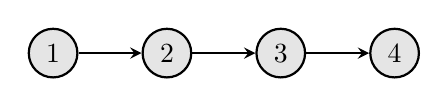
\begin{tikzpicture}
[start chain, every node/.style={draw, circle,minimum size=6mm, fill=gray!20!},
  node distance=8mm, every join/.style={>=stealth,->},
 thick]
\node [draw,on chain,join] {1};
\node [draw,on chain,join] {2};
\node [draw,on chain,join] {3};
\node [draw,on chain,join] {4};
\end{tikzpicture}

$k = 5$

\textbf{Output}:

5 equal parts: \fcj{[[1], [2], [3], [4], null]}

\end{figure}
\end{flushleft}

\paragraph{Example 2:}
\begin{flushleft}


\textbf{Input}:

\fcj{root = [1, 2, 3]}, $k = 5$

\textbf{Output}: \fcj{[[1],[2],[3],[],[]]}

\textbf{Explanation}:

The input and each element of the output are \fcj{ListNodes}, not arrays.

For example, the input root has 

\fcj{root.val = 1}, 

\fcj{root.next.val = 2}, 

\fcj{root.next.next.val = 3}, and 

\fcj{root.next.next.next = null}.

The first element \fcj{output[0]} has \fcj{output[0].val = 1}, \fcj{output[0].next = null}.

The last element \fcj{output[4] is null}, but it's string representation as a ListNode is [].

\end{flushleft}

\paragraph{Example 2:}

\begin{flushleft}

\textbf{Input}: 


\fcj{root = [1, 2, 3, 4, 5, 6, 7, 8, 9, 10]}, $k = 3$

\textbf{Output}: \fcj{[[1, 2, 3, 4], [5, 6, 7], [8, 9, 10]]}

\textbf{Explanation}:

The input has been split into consecutive parts with size difference at most 1, and earlier parts are a larger size than the later parts.

\end{flushleft}

\paragraph{Note:}

\begin{itemize}
\item The length of \fcj{root} will be in the range \fcj{[0, 1000]}.
\item Each value of a node in the input will be an integer in the range \fcj{[0, 999]}.
\item $k$ will be an integer in the range $[1, 50]$.
\end{itemize}

\subsection{Split Input List}
If there are $N$ nodes in the linked list root, then there are $N / k$ items in each part, plus the first $\bmod(N, k)$ parts have an extra item. We can count $N$ with a simple loop.

Now for each part, we will try to set the first $r$ parts has length $N/k + 1$ and remaining with $N/k$. We can directly split the input list.

\setcounter{lstlisting}{0}
\begin{lstlisting}[style=customc, caption={Split Input List}]
vector<ListNode*> splitListToParts( ListNode* root, int k )
{
    auto node = root;
    //get total nodes in the list
    int len = 0;
    while( node )
    {
        ++len;
        node = node->next;
    }

    //q will be number of nodes each part at least have
    int q = len / k;
    //first r parts will have (q+1) nodes
    int r = len - k * q;

    auto start = root;

    vector<ListNode*> ans;
    ans.reserve( k );

    while( k )
    {
        if( start == nullptr )
        {
            break;
        }
        auto partEnd = start;

        int count = q;
        //set first (r) parts
        //have (q+1) nodes
        if( r > 0 )
        {
            ++count;
            --r;
        }
        //the last node of this part
        auto last = partEnd;
        //split the part
        //from start to (start+count-1)
        for( int x = 0; x < count; ++x )
        {
            if( !partEnd )
            {
                //make sure we are not
                //at the end of the list
                break;
            }
            last = partEnd;
            partEnd = partEnd->next;
        }
        //set the part's end node
        //to null pointer
        last->next = nullptr;
        ans.push_back( start );
        //the start of next part
        start = partEnd;
        --k;
    }

    //we have consumed all nodes
    //now add null list
    while( k )
    {
        ans.push_back( nullptr );
        --k;
    }
    return ans;
}
\end{lstlisting}

%\section{726 --- Number of Atoms}
Given a chemical \fcj{formula} (given as a string), return the count of each atom.

An atomic element always starts with an uppercase character, then zero or more lowercase letters, representing the name.

1 or more digits representing the count of that element may follow if the count is greater than 1. If the count is 1, no digits will follow. For example, \textbf{H2O} and \textbf{H2O2} are possible, but \textbf{H1O2} is impossible.

Two formulas concatenated together produce another formula. For example, \textbf{H2O2He3Mg4} is also a formula.

A formula placed in parentheses, and a count (optionally added) is also a formula. For example, \textbf{(H2O2)} and \textbf{(H2O2)3} are formulas.

Given a formula, output the count of all elements as a string in the following form: the first name (in sorted order), followed by its count (if that count is more than 1), followed by the second name (in sorted order), followed by its count (if that count is more than 1), and so on.

\paragraph{Example 1:}

\begin{flushleft}
\textbf{Input}: \fcj{formula = "H2O"}

\textbf{Output}: \fcj{"H2O"}

\textbf{Explanation}: 

The count of elements are \fcj{['H': 2, 'O': 1]}.
\end{flushleft}

\paragraph{Example 2:}

\begin{flushleft}

\textbf{Input}: \fcj{formula = "Mg(OH)2"}

\textbf{Output}: \fcj{"H2MgO2"}

\textbf{Explanation}: 

The count of elements are \fcj{['H': 2, 'Mg': 1, 'O': 2]}.
\end{flushleft}

\paragraph{Example 3:}

\begin{flushleft}
\textbf{Input}: \fcj{formula = "K4(ON(SO3)2)2"}

\textbf{Output}: \fcj{"K4N2O14S4"}

\textbf{Explanation}: 

The count of elements are \fcj{['K': 4, 'N': 2, 'O': 14, 'S': 4]}.
\end{flushleft}

\paragraph{Note:}

\begin{itemize}
\item All atom names consist of lowercase letters, except for the first character which is uppercase.
\item The length of \fcj{formula} will be in the range \fcj{[1, 1000]}.
\item \fcj{formula} will only consist of letters, digits, and round parentheses, and is a valid formula as defined in the problem.
\end{itemize}

\subsection{Recursion}
We will use a helper function, say \fcj{parse}, to parse the \fcj{formula} from index $x$, returning a hash map $M$ which map the element name to their counts.

For the same elements are at the same level (i.e, they are not inside any parenthesis), we will add their counts. When we finish parse a expression inside a parenthesis, we will multiple each name's count by the number immediately following the closing parenthesis.

\begin{itemize}
\item When we see a \fcj{'('}, we will parse whatever is inside the parenthesis (up to the closing one) and add acquired names and count to $M$.
\item Otherwise, we should see an uppercase character: we will parse the rest of the letters to get the name, and add the count to the existing name in $M$.
\item At the end, if there is a final count (representing the multiplicity of a bracketed sequence), we'll multiply each name's count in $M$ by this number.
\end{itemize}

\setcounter{lstlisting}{0}
\begin{lstlisting}[style=customc, caption={Recursion}]
string countOfAtoms( string formula )
{
    string_view sv( formula.c_str(), formula.size() );

    //x will be changed during parsing
    size_t x = 0;
    auto M = parse( sv, x );

    //output to string
    string ans;
    for( const auto& mp : M )
    {
        ans += mp.first;
        if( mp.second > 1 )
        {
            ans += to_string( mp.second );
        }
    }
    return ans;
}

map<string_view, int> parse( string_view s, size_t& x )
{
    map<string_view, int> M;

    while( ( x < s.size() ) && ( s[x] != ')' ) )
    {
        if( s[x] == '(' )
        {
            //the inside expression
            //starting from next index
            ++x;

            //parse inside expression
            //get inside map
            auto y_inside = parse( s, x );

            for( const auto& inside : y_inside )
            {
                M[inside.first] += inside.second;
            }
        } //end if (s[x]==')')
        else
        {
            //parse name
            //s[x] will be uppercase
            //record current x as x0
            //starting x from next
            auto x0 = x;
            ++x;
            while( ( x < s.size() ) && ( is_lowercase( s[x] ) ) )
            {
                ++x;
            }
            //the element name
            auto name = s.substr( x0, x - x0 );
            //parse the digit
            x0 = x;
            while( ( x < s.size() ) && ( is_digit( s[x] ) ) )
            {
                ++x;
            }
            int mul = x0 < x ? to_int( s, x0, x ) : 1;

            //add to dictionary
            //we may have name already appeared
            //add the count togther because
            //there are at same level
            M[name] += mul;
            //now s[x] is a uppercase or ')' or '('
            //continue the while loop
        }//end else
    }//end while

    //if s[x] is ')', it must be the last letter
    //int s, because previous ')' is processed
    //recursively
    //we will parse after x
    //to check if there is a number following
    //the closing parenthesis

    ++x;
    auto x0 = x;
    while( ( x < s.size() ) && ( is_digit( s[x] ) ) )
    {
        ++x;
    }

    if( x0 < x )
    {
        int mul = to_int( s, x0, x );
        //since the number is following the
        //closing parenthesis, we will multiply
        //the number with each name's count
        for( auto& mp : M )
        {
            mp.second *= mul;
        }
    }
    return M;
} //end function

//helper functions
bool is_lowercase( char c )
{
    return ( c >= 'a' ) && ( c <= 'z' );
}
bool is_digit( char c )
{
    return ( c >= '0' ) && ( c <= '9' );
}
int to_int( string_view sv, size_t start, size_t end )
{
    int x = 0;
    for( size_t i = start; i < end; ++i )
    {
        x = x * 10 + ( sv[i] - '0' );
    }
    return x;
}
\end{lstlisting}

\paragraph{Related Problems}
\begin{itemize}
\item \textbf{394. Decode String}
\item \textbf{471. Encode String with Shortest Length}
\item 
\end{itemize}
%\section{727 --- Minimum Window Subsequence}
Given strings $ S $ and $ T $, find the minimum (contiguous) \textbf{substring} $ W $ of $ S $, so that $ T $ is a \textbf{subsequence} of $ W $.

If there is no such window in $ S $ that covers all characters in $ T $, return the empty string \fcj{""}. If there are multiple such minimum-length windows, return the one with the left-most starting index.

\paragraph{Example 1:}

\begin{flushleft}
\textbf{Input}: $S$: \fcj{"abcdebdde"}, $T$: \fcj{"bde"}

\textbf{Output}: \fcj{"bcde"}

\textbf{Explanation}:
 
\fcj{"bcde"} is the answer because it occurs before \fcj{"bdde"} which has the same length.

\fcj{"deb"} is not a smaller window because the elements of $ T $ in the window must occur in order.
\end{flushleft}
 

\paragraph{Note:}

\begin{itemize}
\item All the strings in the input will only contain lowercase letters.
\item The length of S will be in the range \fcj{[1, 20000]}.
\item The length of T will be in the range \fcj{[1, 100]}.

\end{itemize}
\subsection{Two Indexes Sliding Window}
We can make use of a sliding window approach framework, but something is tricky here.

This is: when finding a sliding window that contains $T$, we need to trace back from the right edge of the sliding window back to see if we can shrink the window.

And then, we need to start the right edge of sliding window from the next index of current left edge.

\setcounter{lstlisting}{0}
\begin{lstlisting}[style=customc, caption={Sliding Window}]
string minWindow( string S, string T )
{
    string_view sv( S.c_str(), S.size() );

    size_t ti = 0;

    size_t left = 0;

    string_view best;

    size_t best_len = S.size();

    for( size_t right = 0; right < S.size(); )
    {
        if( T[ti] != sv[right] )
        {
            //only increment index
            //in S
            ++right;
            continue;
        }
        //increment index
        //in T
        ++ti;

        if( ti == T.size() )
        {
            //T is matched completely
            //we need to backtrace from current s[right] and t[ti]
            auto x = right + 1;
            auto y = T.size();

            //since x and y are size_t type
            //we need to not use y>=0 or x >= left
            //[important]: the process of trace back
            while( ( x > left ) && ( y > 0 ) )
            {
                if( sv[x - 1] == T[y - 1] )
                {
                    --y;
                }

                --x;
            }
            //now left is the left edge
            //of shrinked window
            left = x;
            //update minimum length
            //and get the related string
            if( right - left + 1 < best_len )
            {
                best = sv.substr( left, right - left + 1 );
                best_len = right - left + 1;
            }
            //reset index in T to zero
            ti = 0;
            //[important]: set right to the next index of left
            //since we may find another smaller window
            //starting from left+1
            right = left + 1;
        }
        else
        {
            //T has not been matched completely
            //continue incrementing index in S
            ++right;
        }
    }
    return { best.data(), best.size() };
}
\end{lstlisting}
%\include{728}
%\section{729 --- My Calendar I}
Implement a \fcj{MyCalendar} class to store your events. A new event can be added if adding the event will not cause a double booking.

Your class will have the method, \fcj{book(int start, int end)}. Formally, this represents a booking on the half open interval \fcj{[start, end)}, the range of real numbers $x$ such that \fcj{start <= x < end}.

A double booking happens when two events have some non-empty intersection (ie., there is some time that is common to both events.)

For each call to the method \fcj{MyCalendar.book}, return \fcj{true} if the event can be added to the calendar successfully without causing a double booking. Otherwise, return \fcj{false} and do not add the event to the calendar.

Your class will be called like this: 

\fcj{MyCalendar cal = new MyCalendar(); MyCalendar.book(start, end)}

\paragraph{Example 1:}
\begin{flushleft}


\fcj{MyCalendar();}

\fcj{MyCalendar.book(10, 20); // returns true}

\fcj{MyCalendar.book(15, 25); // returns false}

\fcj{MyCalendar.book(20, 30); // returns true}


\textbf{Explanation}:
 
The first event can be booked.  The second can't because time 15 is already booked by another event.

The third event can be booked, as the first event takes every time less than 20, but not including 20.

\end{flushleft}

\paragraph{Note:}

\begin{itemize}
\item The number of calls to \fcj{MyCalendar.book} per test case will be at most 1000.
\item In calls to \fcj{MyCalendar.book(start, end)}, start and end are integers in the range $[0, 10^9]$.
\end{itemize}

\subsection{Binary Search}
If we maintained all events in sorted order, we could check whether an event could be booked in $O(\log N)$ time (where $N$ is the number of events already booked) by binary searching for where the event should be placed. We would also have to insert the event in our sorted structure.

\setcounter{lstlisting}{0}
\begin{lstlisting}[style=customc, caption={Binary Search}]
class MyCalendar
{
public:
    MyCalendar() {}

    bool book( int start, int end )
    {
        if( x_events.empty() )
        {
            x_events.emplace( start, end );
            return true;
        }
        //find the first event
        //lies right of [start,end]
        auto x_low = x_events.lower_bound( start );

        if( x_low != x_events.end() )
        {
            if( x_low->first < end )
            {
                //overlap
                return false;
            }
        }

        if( x_low != x_events.begin() )
        {
            //check the last event
            //lies left of [start,end]
            --x_low;

            if( start < x_low->second )
            {
                //overlap
                return false;
            }
        }

        x_events.emplace( start, end );
        return true;
    }

    map<int, int> x_events;
};
\end{lstlisting}
%
%\section{730 --- Count Different Palindromic Subsequences}
Given a string $S$, find the number of different non-empty palindromic sub-sequences in S, and return that number modulo $10^9 + 7$.

A sub-sequence of a string S is obtained by deleting 0 or more characters from S.

A sequence is palindromic if it is equal to the sequence reversed.

Two sequences $A_1$, $A_2$, $\ldots$ and $B_1$, $B_2$, $\ldots$ are different if there is some $i$ for which $A_i \neq B_i$.

\paragraph{Example 1:}
\begin{flushleft}


\textbf{Input}:
 
$S$: \fcj{'bccb'}

\textbf{Output}: 6

\textbf{Explanation}:
 
The 6 different non-empty palindromic subsequences are \fcj{'b', 'c', 'bb', 'cc', 'bcb', 'bccb'}.

Note that \fcj{'bcb'} is counted only once, even though it occurs twice.

\end{flushleft}

\paragraph{Example 2:}
\begin{flushleft}


\textbf{Input}:
 
$S$: \fcj{'abcdabcdabcdabcdabcdabcdabcdabcddcbadcbadcbadcbadcbadcbadcbadcba'}

\textbf{Output}: \textbf{104860361}

\textbf{Explanation}:
 
There are \textbf{3104860382} different non-empty palindromic subsequences, which is $104860361$ modulo $10^9 + 7$.
\end{flushleft}

\paragraph{Note:}

\begin{itemize}
\item The length of $S$ will be in the range \fcj{[1, 1000]}.
\item Each character $S[i]$ will be in the set \fcj{['a', 'b', 'c', 'd']}.
\end{itemize}

\subsection{Dynamic Programming By Three Dimensional Array}
Suppse $F(x,i,j)$ be the answer for the substring \fcj{S[i,j]} where \fcj{S[i] = S[j] = 'a' + x}. Since we only have 4 characters a, b, c and d, $0 \leq x < 4$. The recursive formula goes as follows:

\begin{itemize}
\item If \fcj{S[i] != 'a'+x}, $F(x,i,j) = F(x,i+1,j)$, note that here we don't include the first character \fcj{S[i]} due to our definition of $F(x,i,j)$.

\item If \fcj{S[j] != 'a'+x}, $F(x,i,j) = F(x, i, j-1)$, not including the last letter \fcj{S[j]}.

\item If \fcj{S[i] == S[j] == 'a'+x}, $F(x,i,j) = 2 + \sum\limits_{y=0}^{3}F(y, i+1,j-1)$. When the first and last characters are the same, we need to count all the distinct palindromes (for each of a, b, c and d) within the sub-window \fcj{S[i+1][j-1]} plus the 2 palindromes contributed by the first and last characters.

\end{itemize}

The final answer would be $\bmod(\sum\limits_{y=0}^{3}F(y,0,n-1), 1000000007)$ where $n$ is the length of the input string $S$. 

\setcounter{lstlisting}{0}
\begin{lstlisting}[style=customc, caption={3D DP}]
int countPalindromicSubsequences( string S )
{
    using v2d_t = vector<vector<int>>;

    vector<v2d_t> F( 4 );

    for( int i = 0; i < 4; ++i )
    {
        v2d_t tmp( S.size(), vector<int>( S.size(), 0 ) );
        F[i].swap( tmp );
    }

    //length = 1
    for( size_t i = 0; i < S.size(); ++i )
    {
        int x = S[i] - 'a';
        F[x][i][i] = 1;
    }

    //length = 2
    for( size_t i = 0; i < S.size() - 1; ++i )
    {
        int x = S[i] - 'a';
        int y = S[i + 1] - 'a';

        if( x == y )
        {
            //('aa') will have ('a', 'aa')
            //we only keep unique string
            F[x][i][i + 1] = 2;
        }
        else
        {
            //need to update F[x][i][i+1]
            //and F[y][i][i+1]
            F[x][i][i + 1] = F[x][i][i];
            F[y][i][i + 1] = F[y][i + 1][i + 1];
        }
    }

    for( size_t l = 3; l <= S.size(); ++l )
    {
        for( size_t i = 0; i + l <= S.size(); ++i )
        {
            auto j = i + l - 1;

            int x = S[i] - 'a';
            int y = S[j] - 'a';

            //we need to check and update (a), (b), (c) and (d)
            for( int ch = 0; ch < 4; ++ch )
            {
                if( x != ch )
                {
                    F[ch][i][j] = F[ch][i + 1][j];
                }
                else if( y != ch )
                {
                    F[ch][i][j] = F[ch][i][j - 1];
                }
                else
                {
                    //we want to find number of subsequence
                    //so x=y bring two palindrom subsequences
                    //S[i]/S[j] and (S[i],S[j])
                    F[ch][i][j] = 2;

                    //We have to add all of the valid palindromes
                    //between S[i+1,j-1]
                    for( int k = 0; k < 4; ++k )
                    {
                        F[ch][i][j] = bmod( F[ch][i][j] + F[k][i + 1][j - 1] );
                    }
                }

            }
        }//for(i)
    } //for(l)

    int ans = 0;

    for( int k = 0; k < 4; ++k )
    {
        ans = bmod( ans + F[k][0][S.size() - 1] );
    }

    return ans;
}

int bmod( int x )
{
    return x % 1000000007;
}
\end{lstlisting}

\subsection{Dynamic Programming By Two Dimensional Array}
Almost every palindrome is going to take one of these four forms: $a\ldots a$, $b\ldots b$, $c\ldots c$, or $d\ldots d$, where $\ldots$ represents a palindrome of zero or more characters. (The only other palindromes are a, b, c, d, and the empty string.)

Let's try to count palindromes of the form $a\ldots a$ (the other types are similar). Suppose $F(i, j)$ be the number of palindromes (including the empty string) in the string $T = S[i, j]$. To count palindromes in $T$ of the form $a\ldots a$, we will need to know the first and last occurrence of \fcj{'a'} in this string. We can make use of another 2D array $N$ whose entry $N(i,0)$ will be the next occurrence of \fcc{'a'} in \fcj{S[i:]}, $N(i,1)$ will be the next occurrence of \fcj{'b'} in \fcj{S[i:]}, and so on.

Also, we will need to know the number of unique letters in $T$ to count the single letter palindromes. We can use the information from $N$ to deduce it: if $N(i,0)$ is $\in [i, j]$, then \fcj{'a'} occurs in $T$, and so on.

There are many duplicate states $F(i,j)$ do not need to be computed, we could make use of a top-down variation of dynamic programming.
%\include{731}
%\section{732 --- My Calendar III}
Implement a \fcj{MyCalendarThree} class to store your events. A new event can \textbf{always} be added.

Your class will have one method, \fcj{book(int start, int end)}. Formally, this represents a booking on the half open interval \fcj{[start, end)}, the range of real numbers $x$ such that \fcj{start <= x < end}.

A $K$--booking happens when $K$ events have some non-empty intersection (i.e., there is some time that is common to all K events.)

For each call to the method \fcj{MyCalendar.book}, return an integer $K$ representing the largest integer such that there exists a $K$-booking in the calendar.

Your class will be called like this: 

\fcj{MyCalendarThree cal = new MyCalendarThree();}

\fcj{MyCalendarThree.book(start, end)}

\paragraph{Example 1:}
\begin{flushleft}


\fcj{MyCalendarThree();}

\fcj{MyCalendarThree.book(10, 20); // returns 1}

\fcj{MyCalendarThree.book(50, 60); // returns 1}

\fcj{MyCalendarThree.book(10, 40); // returns 2}

\fcj{MyCalendarThree.book(5, 15); // returns 3}

\fcj{MyCalendarThree.book(5, 10); // returns 3}

\fcj{MyCalendarThree.book(25, 55); // returns 3}


\textbf{Explanation}: 

The first two events can be booked and are disjoint, so the maximum $K$--booking is a 1--booking.

The third event [10, 40) intersects the first event, and the maximum $ K $--booking is a 2--booking.

The remaining events cause the maximum $K$--booking to be only a 3--booking.

Note that the last event locally causes a 2--booking, but the answer is still 3 because

eg. \fcj{[10, 20)}, \fcj{[10, 40)}, and \fcj{[5, 15)} are still triple booked.
\end{flushleft}
 

\paragraph{Note:}

\begin{itemize}
\item The number of calls to \fcj{MyCalendarThree.book} per test case will be at most 400.
\item In calls to \fcj{MyCalendarThree.book(start, end)}, start and end are integers in the range $[0, 10^9]$.

\end{itemize}

\subsection{Boundary Count}
When booking a new event \fcj{[start, end)}, count \fcj{delta[start]++} and \fcj{delta[end]--}. When processing the values of \fcj{delta} in sorted order of their keys, the largest such value is the answer.

\setcounter{lstlisting}{0}
\begin{lstlisting}[style=customc, caption={Boundary Count}]
class MyCalendarThree
{
public:
    int book( int start, int end );
private:
    map<int, int> delta;
};
//book(int start,int end) implementation
int MyCalendarThree::book( int start, int end )
{
    //increments the count for <start>
    delta[start] += 1;
    //decrements the count for <end>
    delta[end] -= 1;
    //for any start, active_ranges plus 1
    //for any end, active_ranges minus 1
    int active_ranges = 0;
    //the maximum number of overlapped ranges
    int ans = 0;
    //go over the whole end-points
    //maximum number of overlapped ranges
    for( auto it = delta.begin(); it != delta.end(); ++it )
    {
        active_ranges += it->second;
        ans = ( max )( active_ranges, ans );
    }
    return ans;
}
\end{lstlisting}

\subsection{Dynamic Segment Tree By Lazy Propagation}
First, we need to define tree node: A segment tree node typically contains four pieces of information:

\begin{enumerate}
\item The range of a node represents: $[l, r]$ (both inclusive)

\item The properties associated with this segment: for this problem, we define two properties:

\begin{enumerate}
\item $K$: Maximum of overlapped bookings within range $[l, r]$.
\item \fcj{lazy}: this is used for efficient updating.
\end{enumerate}
\item The pointer to the left and right subtrees: \fcj{left} and \fcj{right}.
\end{enumerate}

Here is what a typical segment tree type declaration looks like

\begin{lstlisting}[style=customc]
struct SegTree
{
    int tl;
    int tr;
    int K = 0;
    int lazy = 0;
    SegTree* left = nullptr;
    SegTree* right = nullptr;

    SegTree( int tl_, int tr_ )
        : tl( tl_ ), tr( tr_ )
    {}
};
\end{lstlisting}

Next, we will provide \fcj{update} and \fcj{query} functions.

For this problem, Given a range $[i, j]$, corresponding to an booking of range $[i, j+1)$, the \fcj{query} function should return the maximum number of overlapped bookings, $K$.

The \fcj{update} function will update all segments within the given booking range $[i, j]$ (in this problem, increase the $K$ value of all segments within the range $[i, j]$ by 1).

For \fcj{query} function, we first apply possible lazy propagation. Then, check the query range $[s,e]$ relation to the segment of current node $[l,r]$.

\begin{enumerate}
\item If $[s,e]$ and $[l,r]$ are not intersected, does nothing.
\item If $[l,r]$ is completed inside $[s,e]$, return current node's property (such as $K$ in this problem).
\item Otherwise, $[l,r]$ and $[s,e]$ are partially overlapped, we will recursively calling \fcj{query} on two child nodes of current node for the same query range $[s,e]$
\end{enumerate}

Here is an example of \fcj{query}

\begin{lstlisting}[style=customc]
int query( SegTree* node, int s, int e )
{
    node->propgateLazy();

    if( node->tl > node->tr )
    {
        return 0;
    }

    if( ( node->tl > e ) || ( node->tr < s ) )
    {
        return 0;
    }

    if( ( node->tl >= s ) && ( node->tr <= e ) )
    {
        return node->K;
    }

    //overlap
    int q_left = query( node->getLeft(), s, e );
    int q_right = query( node->getRight(), s, e );

    return ( max )( q_left, q_right );
}
\end{lstlisting}

Function \fcj{update} is very similar to \fcj{query}. Started by propagate lazy, and then we check the segment $[l,r]$ of current node against the query range $[s,e]$.

\begin{enumerate}
\item If both are not intersected, do nothing.
\item If $[l,r]$ is completed inside $[s,e]$, update current segment node and mark its child nodes as lazy.
\item Otherwise, recursively update the child nodes of current node. Then, update current node's property from its child nodes (such as get maximum $K$ from child nodes).
\end{enumerate}

Here is an example of \fcj{update}

\begin{lstlisting}[style=customc]
void update( SegTree* node, int s, int e, int val )
{
    node->propgateLazy();

    if( node->tl > node->tr )
    {
        return;
    }
    if( ( node->tl > e ) || ( node->tr < s ) )
    {
        return;
    }

    //segment inside query range [s,e]
    if( ( node->tl >= s ) && ( node->tr <= e ) )
    {
        node->K += val;

        //mark child nodes as lazy
        if( node->tl != node->tr )
        {
            node->getLeft()->lazy += val;
            node->getRight()->lazy +=  val;
        }
        return;
    }

    auto left_tree = node->getLeft();
    auto right_tree = node->getRight();

    update( left_tree, s, e, val );
    update( right_tree, s, e, val );

    node->K = ( max )( left_tree->K, right_tree->K );
}
\end{lstlisting}

For the lazy propagation, the general steps are listed as following
\begin{enumerate}
\item Update current segment node if it is marked lazy. (In this problem, a node is considered lazy if its \fcj{lazy} property is greater than 0), and the updating is done by adding the \fcj{lazy} to $K$.

\item Push the laziness down to the child nodes: first make sure current segment node is not a leaf node (a leaf node has $l = r$), then update the child nodes' \fcj{lazy}.

\item Reset the laziness of current segment node (In this problem, we reset \fcj{lazy} to 0).
\end{enumerate}

\begin{lstlisting}[style=customc]
void propgateLazy( SegTree* node )
{
    if( node->lazy != 0 )
    {
        //1. update current node
        node->K += node->lazy;

        //2. check if it is a leaf
        if( tl != tr )
        {
            //push down the laziness
            //to the child nodes
            node->getLeft()->lazy += lazy;
            node->getRight()->lazy += lazy;
        }
        //3. reset lazy of current node
        node->lazy = 0;
    }
}
\end{lstlisting}

Finally, we initialize the root node: The root node should at least cover the maximum range allowed for all events. In this problem, this is $[0, 10^9]$. The root node's $K$ and \fcj{lazy} are set to 0.

\begin{lstlisting}[style=customc, caption={Segment Tree}]
class MyCalendarThree
{
public:
    MyCalendarThree()
    {
        d_root = new SegTree( 0, 1000000100 );
    }

    int book( int start, int end )
    {
        //update segment tree by this new range
        update( d_root, start, end - 1, 1 );
        //then query the maximum K in the whole range
        return query( d_root, 0, 1000000100 );
    }
private:
    struct SegTree
    {
        int tl;
        int tr;
        int K = 0;
        int lazy = 0;
        SegTree* left = nullptr;
        SegTree* right = nullptr;

        SegTree( int tl_, int tr_ )
            : tl( tl_ ), tr( tr_ )
        {}

        int mid()
        {
            return ( tl + tr ) / 2;
        }

        SegTree* getLeft()
        {
            if( !left )
            {
                left = new SegTree( tl, mid() );
            }

            return left;
        }

        SegTree* getRight()
        {
            if( !right )
            {
                right = new SegTree( mid() + 1, tr );
            }

            return right;
        }

        void propgateLazy()
        {
            if( lazy )
            {
                K += lazy;
                if( tl != tr )
                {
                    getLeft()->lazy += lazy;
                    getRight()->lazy += lazy;
                }
                lazy = 0;
            }
        }
    };

    void update( SegTree* node, int s, int e, int val )
    {
        node->propgateLazy();

        if( node->tl > node->tr )
        {
            //current node's segment
            //does not intersect with query range
            return;
        }
        if( ( node->tl > e ) || ( node->tr < s ) )
        {
            //current node's segment
            //is completely inside query range
            return;
        }

        if( ( node->tl >= s ) && ( node->tr <= e ) )
        {
            node->K += val;

            //for non-leaf node
            if( node->tl != node->tr )
            {
                //makr its child nodes as lazy
                node->getLeft()->lazy += val;
                node->getRight()->lazy +=  val;
            }
            return;
        }

        auto left_tree = node->getLeft();
        auto right_tree = node->getRight();

        update( left_tree, s, e, val );
        update( right_tree, s, e, val );

        node->K = ( max )( left_tree->K, right_tree->K );
    }

    int query( SegTree* node, int s, int e )
    {
        node->propgateLazy();

        if( node->tl > node->tr )
        {
            return 0;
        }

        if( ( node->tl > e ) || ( node->tr < s ) )
        {
            //current node's segment
            //does not intersect with query range
            return 0;
        }

        if( ( node->tl >= s ) && ( node->tr <= e ) )
        {
            //current node's segment
            //is completely inside query range
            return node->K;
        }

        //overlap
        int q_left = query( node->getLeft(), s, e );
        int q_right = query( node->getRight(), s, e );

        return ( max )( q_left, q_right );
    }

    SegTree* d_root;
};
\end{lstlisting}

\subsection{Count Time Points}
In this approach, we find the affected ranges by counting each booked start and end time with a tree map $M$.

For a current booking time $[s,e]$, locate the smallest time point $x$ which is no less than the \fcj{start}. We go to the previous node of $x$: $x_0$. Then insert $s$ into $M$ with $x_0$'s count, and get the position of $s$ in $M$, say $l$. If $s$ is already in $M$, the function \fcc{emplace} just return the position of the current $s$. 

Using the same manner to insert $e$ into $M$, and get the position of $e$ in $M$.

Then, we iterate from $l$ to previous position of $r$ and increments the count of each associated time point. In this way, we always ignore $e$ when updating. By taking the previous one's count as current time point's count, we don't need to go over from the whole time points again since later inserted time point has the count of its closest one remembered.

To help the location of smallest time point that is no less than the one we are querying, we can pre-insert $(-1,0)$ into $M$. Thus, we can always get this smallest time point.

Also, $K$ is a global variable and updated for each call to \fcj{book}

\begin{lstlisting}[style=customc, caption={Counting Time Points}]
class MyCalendarThree
{
public:
    MyCalendarThree()
    {
        //(-1,0) help us
        //free of checking if it is the begin node
        delta.emplace( -1, 0 );
    }

    int book( int start, int end )
    {
        //find the largest time point
        //which is less than start
        auto x = delta.lower_bound( start );
        auto prev_x = prev( x );
        //insert start into map and taking prev_x's count
        //as its count. In this way, we remembered the count
        //of passing time point prev_x->first
        //no need to count again after
        auto left = delta.emplace( start, prev_x->second ).first;
        //same manner as insert start
        auto y = delta.lower_bound( end );
        auto prev_y = prev( y );

        auto right = delta.emplace( end, prev_y->second ).first;
        //we iterate from left to previous one of right
        //thus we don't counter end
        for( auto it = left; it != right; ++it )
        {
            //since we remembered the count of passing time point
            //prev_x->first, increments each time point's count
            //represents it is affected by current booking time range
            ++it->second;
            //update K accordingly.
            //here K is a global state
            K = ( max )( K, it->second );
        }
        return K;
    }

    map<int, int> delta;
    int K;
};
\end{lstlisting}
%\section{733 --- Flood Fill}
An image is represented by a 2-D array of integers, each integer representing the pixel value of the image (from 0 to 65535).

Given a coordinate \fcj{(sr, sc)} representing the starting pixel (row and column) of the flood fill, and a pixel value \fcj{newColor}, \fcj{"flood fill"} the image.

To perform a \fcj{"flood fill"}, consider the starting pixel, plus any pixels connected 4-direction to the starting pixel of the same color as the starting pixel, plus any pixels connected 4-direction to those pixels (also with the same color as the starting pixel), and so on. Replace the color of all of the aforementioned pixels with the \fcj{newColor}.

At the end, return the modified image.

\paragraph{Example 1:}

\textbf{Input}:
 
\fcj{image = [[1,1,1],[1,1,0],[1,0,1]]}

\fcj{sr = 1}, \fcj{sc = 1}, \fcj{newColor = 2}

\textbf{Output}: \fcj{[[2,2,2],[2,2,0],[2,0,1]]}

\textbf{Explanation}:
 
From the center of the image (with position \fcj{(sr, sc) = (1, 1)}), all pixels connected 

by a path of the same color as the starting pixel are colored with the new color.

Note the bottom corner is not colored 2, because it is not 4-direction connected to the starting pixel.

\paragraph{Note:}
\begin{itemize}
\item The length of \fcj{image} and \fcj{image[0]} will be in the range \fcj{[1, 50]}.

\item The given starting pixel will satisfy \fcj{0 <= sr < image.length} and \fcj{0 <= sc < image[0].length}.

\item The value of each color in \fcj{image[i][j]} and \fcj{newColor} will be an integer in \fcj{[0, 65535]}.

\end{itemize}

\subsection{Depth First Search}
This is an easy problem with Depth First Search.

Note: we only do flood filling when \fcj{image[sr][sc]!=newColor}.

\setcounter{lstlisting}{0}
\begin{lstlisting}[style=customc, caption={Depth First Search}]
vector<vector<int>> floodFill( vector<vector<int>>& image, int sr, int sc, int newColor )
{
    int M = static_cast<int>( image.size() );
    int N = static_cast<int>( image[0].size() );
    if( image[sr][sc] == newColor )
    {
        //if the pixel value at (sr,sc) is equal to newColor
        //no need to do flood fill
        return image;
    }
    flood( image, sr, sc, newColor, image[sr][sc] );
    return image;
}
//DFS helper function
void flood( vector<vector<int>>& G, int r, int c, int color, int gray )
{
    int dr[] = {-1, 0, 1, 0};
    int dc[] = {0, -1, 0, 1};
    int M = static_cast<int>( G.size() );
    int N = static_cast<int>( G[0].size() );
    G[r][c] = color;
    for( int i = 0; i < 4; ++i )
    {
        int nr = r + dr[i];
        int nc = c + dc[i];

        if( ( nr >= 0 ) && ( nr < M ) && ( nc >= 0 ) && ( nc < N ) )
        {
            if( G[nr][nc] == gray )
            {
                flood( G, nr, nc, color, gray );
            }
        }
    }
}
\end{lstlisting}
%\include{734}
%\section{735 --- Asteroid Collision}
We are given an array \fcj{asteroids} of integers representing asteroids in a row.

For each asteroid, the absolute value represents its size, and the sign represents its direction (positive meaning right, negative meaning left). Each asteroid moves at the same speed.

Find out the state of the asteroids after all collisions. If two asteroids meet, the smaller one will explode. If both are the same size, both will explode. Two asteroids moving in the same direction will never meet.

\paragraph{Example 1:}
\begin{flushleft}

\textbf{Input}: 

\fcj{asteroids}: \fcj{[5, 10, -5]}

\textbf{Output}: \fcj{[5, 10]}

\textbf{Explanation}: 

The 10 and $-5$ collide resulting in 10.  The 5 and 10 never collide.
\end{flushleft}
\paragraph{Example 2:}
\begin{flushleft}

\textbf{Input}: 

\fcj{asteroids}: \fcj{[8, -8]}

\textbf{Output}: \fcj{[]}

\textbf{Explanation}: 

The 8 and $-8$ collide exploding each other.
\end{flushleft}
\paragraph{Example 3:}
\begin{flushleft}

\textbf{Input}: \fcj{asteroids = [10, 2, -5]}

\textbf{Output}: \fcj{[10]}

\textbf{Explanation}:
 
The 2 and $-5$ collide resulting in $-5$.  The 10 and $-5$ collide resulting in 10.
\end{flushleft}
\paragraph{Example 4:}
\begin{flushleft}


\textbf{Input}: \fcj{asteroids = [-2, -1, 1, 2]}

\textbf{Output}: \fcj{[-2, -1, 1, 2]}

\textbf{Explanation}:
 
The $-2$ and $-1$ are moving left, while the 1 and 2 are moving right.

Asteroids moving the same direction never meet, so no asteroids will meet each other.
\end{flushleft}

\paragraph{Note:}
\begin{itemize}
\item The length of asteroids will be at most 10000.
\item Each asteroid will be a non-zero integer in the range \fcj{[-1000, 1000]}.
\end{itemize}

\subsection{Stack}
We make use of a stack to track the elements. We notice that only when top of stack is moving right and current element is moving left, the two can meet. Otherwise, they just remain as they are. Thus, we only compare stack elements with current element when current element is negative (moving left).

Finally, we insert all elements in the stack into the output, and then reverse it.

\setcounter{lstlisting}{0}
\begin{lstlisting}[style=customc, caption={Stack}]
vector<int> asteroidCollision( vector<int>& asteroids )
{
    stack<int> stk;
    for( int n : asteroids )
    {
        if( n < 0 )
        {
            //only when n is moving left
            //we may have two asteroids collison
            while( !stk.empty() && ( stk.top() > 0 ) )
            {
                //only when the top is moving right (>0)
                //the collison will happen
                if( stk.top() < abs( n ) )
                {
                    //top is exploded
                    stk.pop();
                }
                else if( stk.top() > abs( n ) )
                {
                    //n is exploded
                    n = 0;
                    break;
                }
                else
                {
                    //both are exploded
                    n = 0;
                    stk.pop();
                    break;
                }
            }
        }
        if( n != 0 )
        {
            //n is not exploded
            //add it to the stack
            stk.push( n );
        }
    }
    //put all remaining asteroids
    //into the output
    vector<int> ans;
    ans.reserve( stk.size() );
    while( !stk.empty() )
    {
        ans.push_back( stk.top() );
        stk.pop();
    }
    //reverse the output
    reverse( begin( ans ), end( ans ) );
    return ans;
}
\end{lstlisting}
%\section{736 --- Parse Lisp Expression}
You are given a string \fcj{expression} representing a Lisp-like expression to return the integer value of.

The syntax for these expressions is given as follows.

\begin{itemize}
\item An expression is either an integer, a let--expression, an add--expression, a mult--expression, or an assigned variable. Expressions always evaluate to a single integer.

\item (An integer could be positive or negative.)

\item A \textbf{let--expression} takes the form \fcj{(let v1 e1 v2 e2 ... vn en expr)}, where \fcj{let} is always the string \fcj{"let"}, then there are 1 or more pairs of alternating variables and expressions, meaning that the first variable \fcj{v1} is assigned the value of the expression \fcj{e1}, the second variable \fcj{v2} is assigned the value of the expression \fcj{e2}, and so on sequentially; and then the value of this \textbf{let--expression} is the value of the expression \fcj{expr}.

\item An \textbf{add--expression} takes the form \fcj{(add e1 e2)} where \fcj{add} is always the string \fcj{"add"}, there are always two expressions \fcj{e1}, \fcj{e2}, and this expression evaluates to the addition of the evaluation of \fcj{e1} and the evaluation of \fcj{e2}.

\item A \textbf{mult--expression} takes the form \fcj{(mult e1 e2)} where \fcj{mult} is always the string \fcj{"mult"}, there are always two expressions \fcj{e1}, \fcj{e2}, and this expression evaluates to the multiplication of the evaluation of \fcj{e1} and the evaluation of \fcj{e2}.

\item For the purposes of this question, we will use a smaller subset of variable names. A variable starts with a lowercase letter, then zero or more lowercase letters or digits. Additionally for your convenience, the names \fcj{"add"}, \fcj{"let"}, or \fcj{"mult"} are protected and will never be used as variable names.

\item Finally, there is the concept of scope. When an expression of a variable name is evaluated, \textbf{within the context of that evaluation}, the innermost scope (in terms of parentheses) is checked first for the value of that variable, and then outer scopes are checked sequentially. It is guaranteed that every expression is legal.

\end{itemize}


\paragraph{Evaluation Examples:}
\begin{flushleft}

\textbf{Input}: \fcj{(add 1 2)}

\textbf{Output}: 3

\textbf{Input}: \fcj{(mult 3 (add 2 3))}

\textbf{Output}: 15

\textbf{Input}: \fcj{(let x 2 (mult x 5))}

\textbf{Output}: 10

\textbf{Input}: \fcj{(let x 2 (mult x (let x 3 y 4 (add x y))))}

\textbf{Output}: 14

\textbf{Explanation}: 

In the expression \fcj{(add x y)}, when checking for the value of the variable $x$, we check from the innermost scope to the outermost in the context of the variable we are trying to evaluate. Since $x = 3$ is found first, the value of x is 3.

\textbf{Input}: \fcj{(let x 3 x 2 x)}

\textbf{Output}: 2

\textbf{Explanation}: Assignment in let statements is processed sequentially.

\textbf{Input}: \fcj{(let x 1 y 2 x (add x y) (add x y))}

\textbf{Output}: 5

\textbf{Explanation}:

The first \fcj{(add x y)} evaluates as 3, and is assigned to $x$.

The second \fcj{(add x y)} evaluates as $3+2 = 5$.

\textbf{Input}: \fcj{(let x 2 (add (let x 3 (let x 4 x)) x))}

\textbf{Output}: 6

\textbf{Explanation}: 

Even though \fcj{(let x 4 x)} has a deeper scope, it is outside the context of the final $x$ in the add-expression.  That final x will equal 2.

\textbf{Input}: \fcj{(let a1 3 b2 (add a1 1) b2) }

\textbf{Output}: 4

\textbf{Explanation}: Variable names can contain digits after the first character.


\end{flushleft}
\paragraph{Note:}

\begin{itemize}
\item The given string \fcj{expression} is well formatted: There are no leading or trailing spaces, there is only a single space separating different components of the string, and no space between adjacent parentheses. The expression is guaranteed to be legal and evaluate to an integer.
\item The length of \fcj{expression} is at most 2000. (It is also non-empty, as that would not be a legal expression.)
\item The answer and all intermediate calculations of that answer are guaranteed to fit in a 32-bit integer.
\end{itemize}

\subsection{Recursive Parsing}
The algorithm is very straightforward with some very tricky points.

The parsing loop is almost same as problem \textbf{726 --- Number Of Atoms}. We will stop the loop when we at \fcj{')'}.

\begin{enumerate}
\item When parsing \fcj{'let'}, we record current found variable and value, and maintain a state to indicate if we are parsing a variable or a number.
\item When parsing \fcj{'add'} or \fcj{'mult'}, we will search the value of the variable in hash maps from inner most to outer most. Thus, we need an array of hash maps to map variable to its value inside each expression.
\item The last expression of \fcj{'let'} need to be evaluated carefully.
\end{enumerate}

\setcounter{lstlisting}{0}
\begin{lstlisting}[style=customc, caption={Recursive Parsing}]
int evaluate( string expression )
{

    size_t start = 0;

    string_view expr( expression.c_str(), expression.size() );

    vector<unordered_map<string_view, int>> dicts;

    return parse( expr, start, dicts );
}

int parse( string_view expr, size_t& start, vector<unordered_map<string_view, int>>& dicts )
{
    //the state of parsing <let>
    //0: parsing a variable
    //1: parsing a number
    unsigned char let_state = 0;

    vector<string_view> vars;
    vector<int> evals;

    dicts.emplace_back( unordered_map<string_view, int> {} );

    char oper = 'z';

    while( ( start < expr.size() ) && ( expr[start] != ')' ) )
    {
        if( expr[start] == '(' )
        {
            ++start;
            int val = parse( expr, start, dicts );

            if( oper == 'z' )
            {
                //this is the outmost level
                //directly return the value
                return val;
            }

            if( oper == 'l' )
            {
                //this is <let>
                if( let_state == 1 )
                {
                    //we are parse number
                    //map last variable to this value
                    dicts.back()[vars.back()] = val;
                    vars.pop_back();
                }
                else
                {
                    //we should parse variable
                    //but found a value
                    //maybe it is the last expression of <let>
                    evals.push_back( val );
                }
                //change state
                let_state = 1 - let_state;
            }
            else
            {
                //<add> and <mult> requires a value
                evals.push_back( val );
            }
        }
        else if( oper == 'z' )
        {
            oper = expr[start];
            //<mult> has four letters
            start += ( oper == 'm' ) ? 5 : 4;
        }
        else if( oper == 'l' )  //let
        {
            size_t p = start;
            //move start until a space, '(' or ')' is met
            while( ( start < expr.size() ) && !is_sep( expr[start] ) )
            {
                ++start;
            }

            bool is_name = is_lc( expr[p] );
            if( is_name )
            {
                //this is a variable name
                vars.emplace_back( expr.substr( p, start - p ) );
            }
            else
            {
                //this is a value
                evals.push_back( to_int( expr, p, start ) );
            }

            if( let_state )
            {
                //we are parsing a value
                if( is_name )
                {
                    //but we are given a variable
                    //thus we will map the value of this variable
                    //to the last variable's value
                    //we need to pop_back() twice
                    //because we have push_back current variable
                    auto var = vars.back();
                    vars.pop_back();

                    dicts.back()[vars.back()] = dicts.back()[var];
                    vars.pop_back();
                }
                else
                {
                    //map the value to the last variable
                    dicts.back()[vars.back()] = evals.back();
                    //we need remove last variable
                    //and current value
                    vars.pop_back();
                    evals.pop_back();
                }
            }
            //change the state
            let_state = 1 - let_state;
            //only advance start when it is space
            if( expr[start] == ' ' )
            {
                ++start;
            }
        }
        else
        {
            auto p = start;
            //move start until a space, '(' or ')' is met
            while( ( start < expr.size() ) && !is_sep( expr[start] ) )
            {
                ++start;
            }

            if( is_lc( expr[p] ) )
            {
                //we got a variable
                auto var = expr.substr( p, start - p );
                //get the value from the hash maps hierachy
                evals.push_back( find_val( dicts, var ) );
            }
            else
            {
                //we got a value
                //save it
                evals.push_back( to_int( expr, p, start ) );
            }
//only advance start when it is space
            if( expr[start] == ' ' )
            {
                ++start;
            }
        }

    } //end while

    int val = -1;

    if( oper == 'l' )
    {
        //we are end of <let>
        if( !evals.empty() )
        {
            //we have expression value
            //as the last
            val = evals.back();
        }
        else
        {
            //we must have a variable as the last one
            val = find_val( dicts, vars.back() );
        }
    }
    else
    {
        //we are at the end of <add> or <mult>
        val = evals.back();
        evals.pop_back();

        if( oper == 'a' )
        {
            val += evals.back();
        }
        else
        {
            val *= evals.back();
        }
    }
    //remove current hash map
    dicts.pop_back();
    //advance index
    ++start;
    if( ( start < expr.size() ) && ( expr[start] == ' ' ) )
    {
        //advance to skip space
        ++start;
    }
    return val;
}//end parse()
//helper function to tranform to integer
int to_int( string_view sv, size_t start, size_t end )
{
    int x = 0;
    int sign = 1;
    auto i = start;
    //need to consider negative number
    if( sv[i] == '-' )
    {
        sign = -1;
        ++i;
    }

    for( ; i < end; ++i )
    {
        x = x * 10 + ( sv[i] - '0' );
    }

    return x * sign;
}

bool is_lc( char c )
{
    return ( c >= 'a' ) && ( c <= 'z' );
}

bool is_sep( char c )
{
    return ( c == ' ' ) || ( c == ')' ) || ( c == '(' );
}
//find value of <var> through
//hash map hierachy
int find_val( vector<unordered_map<string_view, int>>& dicts, string_view var )
{
    for( auto x = dicts.rbegin(); x != dicts.rend(); ++x )
    {
        auto it = x->find( var );
        if( it != x->end() )
        {
            return it->second;
        }
    }
    return 0;
}
\end{lstlisting}

\paragraph{Related Problems}
\begin{itemize}
\item \textbf{439. Ternary Expression Parser}
\item \textbf{726. Number of Atoms}
\item \textbf{770. Basic Calculator IV}
\end{itemize}

%\section{737 --- Sentence Similarity II}
Given two sentences \fcj{words1}, \fcj{words2} (each represented as an array of strings), and a list of similar word pairs \fcj{pairs}, determine if two sentences are similar.

For example, 

\fcj{words1 = ["great", "acting", "skills"]} 

and 

\fcj{words2 = ["fine", "drama", "talent"]} 

are similar, if the similar word pairs are 

\fcj{[["great", "good"], ["fine", "good"], ["acting","drama"], ["skills","talent"]]}.

Note that the similarity relation is transitive. For example, if \fcj{"great"} and \fcj{"good"} are similar, and \fcj{"fine"} and \fcj{"good"} are similar, then \fcj{"great"} and \fcj{"fine"} are similar.

Similarity is also symmetric. For example, \fcj{"great"} and \fcj{"fine"} being similar is the same as \fcj{"fine"} and \fcj{"great"} being similar.

Also, a word is always similar with itself. For example, the sentences 

\fcj{words1 = ["great"]}, \fcj{words2 = ["great"]}, \fcj{pairs = []} are similar, even though there are no specified similar word pairs.

Finally, sentences can only be similar if they have the same number of words. So a sentence like \fcj{words1 = ["great"]} can never be similar to \fcj{words2 = ["doubleplus","good"]}.

\paragraph{Note:}

\begin{itemize}
\item The length of \fcj{words1} and \fcj{words2} will not exceed 1000.
\item The length of \fcj{pairs} will not exceed 2000.
\item The length of each \fcj{pairs[i]} will be 2.
\item The length of each \fcj{words[i]} and \fcj{pairs[i][j]} will be in the range \fcj{[1, 20]}.

\end{itemize}
%\section{738 --- Monotone Increasing Digits}
Given a non-negative integer $N$, find the largest number that is less than or equal to $N$ with monotone increasing digits.

(Recall that an integer has monotone increasing digits if and only if each pair of adjacent digits $x$ and $y$ satisfy $x \leq y$.)

\paragraph{Example 1:}
\begin{flushleft}

\textbf{Input}: $N = 10$

\textbf{Output}: 9
\end{flushleft}

\paragraph{Example 2:}
\begin{flushleft}


\textbf{Input}: $N = 1234$

\textbf{Output}: 1234

\end{flushleft}

\paragraph{Example 3:}
\begin{flushleft}


\textbf{Input}: $N = 332$

\textbf{Output}: 299

\end{flushleft}

\subsection{Greedy}
We construct an array of digits from $N$.

Then, we iterate over the digits array by comparing current digits $x$ against its next digit $y$

\begin{itemize}
\item If $x\leq y$, it meets the monotone increasing condition, thus we move to next digit.
\item Otherwise, we will change all the digits after $x$ to 9 and change $x$ to $x-1$. Then, we need to go back from $x$ to the first digit. During the tracking back, we check if current digit is less than its previous one. If it is, we will change current digit to 9 and decrement previous digit.
\end{itemize}

\setcounter{lstlisting}{0}
\begin{lstlisting}[style=customc, caption={Greedy}]
int monotoneIncreasingDigits( int N )
{
    //expand N to a digit array
    vector<int> digits;
    int n = 0;
    while( N )
    {
        int q = N / 10;
        int r = N - 10 * q;
        digits.push_back( r );
        N = q;
        ++n;
    }
    //reverse the array
    //make sure the highest digit is the first element
    reverse( begin( digits ), end( digits ) );
    for( int i = 0; i < n - 1; ++i )
    {
        if( digits[i] > digits[i + 1] )
        {
            //decrement current digit
            digits[i] -= 1;
            //we will change all the digits
            //after i to 9
            for( int j = i + 1; j < n; ++j )
            {
                digits[j] = 9;
            }
            //make sure from the start to i
            //is still a monoton increasing
            int j = i;
            while( j >= 1 )
            {
                if( digits[j - 1] > digits[j] )
                {
                    //change current digit to 9
                    //decrements previous digit
                    digits[j] = 9;
                    digits[j - 1] -= 1;
                }
                --j;
            }
            break;
        }
    }
    //reconstruct the answer from the array
    int ans = 0;
    for( int d : digits )
    {
        ans = ans * 10 + d;
    }
    return ans;
}
\end{lstlisting}
%\section{739 --- Daily Temperatures}
Given a list of daily temperatures $T$, return a list such that, for each day in the input, tells you how many days you would have to wait until a warmer temperature. If there is no future day for which this is possible, put 0 instead.

For example, given the list of temperatures 

\begin{flushleft}
$T$: \fcj{[73, 74, 75, 71, 69, 72, 76, 73]}, 

your output should be 

\fcj{[1, 1, 4, 2, 1, 1, 0, 0]}.
\end{flushleft}

\paragraph{Note:} 

\begin{itemize}
\item The length of temperatures will be in the range \fcj{[1, 30000]}. 
\item Each temperature will be an integer in the range \fcj{[30, 100]}.
\end{itemize} 

\subsection{Stack}
In this approach, we reversely iterate over $T$. We also make use of a stack $S$ to record indexes. 

During the traversing
\begin{itemize}
\item As long as current temperature $t$ is no less than the temperature at top index of $S$, we will keep popping index from $S$. For each temperature at popped index, $t$ is the first one on its right side, thus, the distance to the index of $t$ is the number of days to get warmer.
\item Then, push current index into $S$.
\end{itemize}

\setcounter{lstlisting}{0}
\begin{lstlisting}[style=customc, caption={Stack}]
vector<int> dailyTemperatures( vector<int>& T )
{
    //base case: empty array
    if( T.empty() )
    {
        return {};
    }
    stack<int> stk;
    vector<int> ans;
    ans.reserve( T.size() );
    int n = static_cast<int>( T.size() );
    //The last temperature has no any day associated
    //thus is zero
    ans.push_back( 0 );
    //push the last index into the stack
    stk.push( n - 1 );
    //reversely traversing T
    for( int i = n - 2; i >= 0; --i )
    {
        while( !stk.empty() && ( T[stk.top()] <= T[i] ) )
        {
            //now T[i] is the first temperature
            //on the right side of T[stk.top()]
            //which is larger than T[stk.top()]
            stk.pop();
        }
        if( stk.empty() )
        {
            //no any temperature is larger than T[i] on
            //its right side
            ans.push_back( 0 );
        }
        else
        {
            //otherwise
            //the difference of indexes is the
            //answer: the number of days
            ans.push_back( stk.top() - i );
        }
        //push current index of temperature into the stack
        stk.push( i );
    }
    //reverse the array since it added from end
    reverse( begin( ans ), end( ans ) );
    return ans;
}
\end{lstlisting}

\subsection{Constant Memory}
Actually, we can make use of result array to solve this problem. Thus we don't need the auxiliary stack. 

We still reversely traverse $T$. Suppose we are at index $i$ and we have filled the result array, say $R$, from $i+1$ to $n-1$ ($n$ is the length of $T$). 

Now to find the most recent day after $i$ which is warmer than $T[i]$, we start searching from $i+1$. If $T[k] \leq T[i]$ for a $k >i$, we don't just move to $k+1$, we can use the result of $R[k]$ to move $k$. Since $T[k]\leq T[i]$, the most recent day that could be warmer than $T[i]$ will be at index $k+R[k]$. After updating $k$ to $k+R[k]$, we repeat the above process. 

If $R[k]=0$, this means $T[k]$ is the highest temperature from $k$. Since $T[k]\leq T[i]$, it is obvious that $R[i]=0$.

\setcounter{lstlisting}{0}
\begin{lstlisting}[style=customc, caption={Constant Memory}]
vector<int> dailyTemperatures( vector<int>& T )
{
    vector<int> ans( T.size(), 0 );
    int n = static_cast<int>( T.size() );
    for( int i = n - 2; i >= 0; --i )
    {
        //search the most recent day after i
        //which is warmer than i
        int j = i + 1;
        while( ( j < n ) && ( T[j] <= T[i] ) )
        {
            if( ans[j] > 0 )
            {
                //we move to j+ans[j]
                //since ans[j] is the most recent day
                //warmer than j
                j = j + ans[j];
            }
            else
            {
                //j has the highest temperature
                //from j
                //thus we break the loop
                j = n;
            }
        }

        if( j == n )
        {
            //since T[j] <=T[i]
            //thus T[i] is the highest temperature
            //from i
            ans[i] = 0;
        }
        else
        {
            //the days will be j-i
            ans[i] = j - i;
        }
    }
    return ans;
}
\end{lstlisting} 


%\section{740 --- Delete and Earn}
Given an array of integers, \fcj{nums}, you can perform operations on the array.

In each operation, you pick any \fcj{nums[i]} and delete it to earn \fcj{nums[i]} points. After, you must delete every element equal to \fcj{nums[i] - 1} or \fcj{nums[i] + 1}.

You start with 0 points. Return the maximum number of points you can earn by applying such operations.

\paragraph{Example 1:}
\begin{flushleft}


\textbf{Input}: \fcj{nums = [3, 4, 2]}

\textbf{Output}: 6

\textbf{Explanation}:
 
Delete 4 to earn 4 points, consequently 3 is also deleted.

Then, delete 2 to earn 2 points. 6 total points are earned.
\end{flushleft}
 

\paragraph{Example 2:}
\begin{flushleft}


\textbf{Input}: \fcj{nums = [2, 2, 3, 3, 3, 4]}

\textbf{Output}: 9

\textbf{Explanation}:
 
Delete 3 to earn 3 points, deleting both 2's and the 4.

Then, delete 3 again to earn 3 points, and 3 again to earn 3 points.

9 total points are earned.
\end{flushleft}
 

\paragraph{Note:}

\begin{itemize}
\item The length of \fcj{nums} is at most 20000.
\item Each element \fcj{nums[i]} is an integer in the range \fcj{[1, 10000]}.
\end{itemize}

\subsection{Dynamic Programming}
To facilitate processing, we put all the elements into a tree map. Suppose before processing current element $x$, we have obtained the points by deleting and not deleting the largest element so far, $y$, which are $D$ (deleting) and $K$ (keep) respectively.

Thus, for each unique value $x$ of \fcj{nums} in increasing order

\begin{itemize}
\item If $x$ is adjacent to the previously largest value $y$, the points that we can obtain by deleting $x$ will be $K+x$(i.e., the points that not deleting $y$ plus the points of $x$). If we don't delete $x$, the points we can obtain will be $\max(D, K)$ (we don't get point if not deleting $x$)
\item Similarly, if $x$ is not adjacent to $y$, then the points we can obtain by deleting $x$ will be $\max(D, K)+x$, and the points by not deleting $x$ be $\max(D, K)$.

\end{itemize}
At the end, the best answer may or may not use the largest value in \fcj{nums}, so we return $\max(D, K)$.

\setcounter{lstlisting}{0}
\begin{lstlisting}[style=customc, caption={Dynamic Programming}]
int deleteAndEarn( vector<int>& nums )
{
    if( nums.empty() )
    {
        return 0;
    }
    map<int, int> dict;
    for( int n : nums )
    {
        dict[n] += 1;
    }
    auto it = dict.begin();
    //the points obtained by earning the point from current one
    int D = get<0>( *it ) * get<1>( *it );
    //the points obtained by not earning the point from current one
    int K = 0;
    //the last largest value
    int y = get<0>( *it );
    ++it;
    for( ; it != dict.end(); ++it )
    {
        int x = get<0>( *it );
        int last_D = D;
        int last_K = K;
        if( x == y + 1 )
        {
            //if we want to earn the points from x,
            //y must be deleted without earning the point
            D = x * get<1>( *it ) + last_K;
            //if we don't want to earn the points from x,
            //we can either choose obtaining from y or not from y
            K = ( max )( last_K, last_D );
        }
        else
        {
            //if we want to earn the points from x,
            //y don't need to be deleted
            D =  x * get<1>( *it ) + ( max )( last_K, last_D );
            //if we don't want to earn the points from x,
            //we can either choose obtaining from y or not from y
            K = ( max )( last_K, last_D );
        }
        //update largest element so far
        y = x;
    }
    return ( max )( D, K );
}
\end{lstlisting}
%\section{741 --- Cherry Pickup}
In a $N \times N$ \fcj{grid} representing a field of cherries, each cell is one of three possible integers.

\begin{itemize}
\item 0 means the cell is empty, so you can pass through;
\item 1 means the cell contains a cherry, that you can pick up and pass through;
\item $-1$ means the cell contains a thorn that blocks your way.
\end{itemize}

Your task is to collect maximum number of cherries possible by following the rules below:
\begin{itemize}
\item Starting at the position (0, 0) and reaching $(N-1, N-1)$ by moving right or down through valid path cells (cells with value 0 or 1);
\item After reaching $(N-1, N-1)$, returning to (0, 0) by moving left or up through valid path cells;
\item When passing through a path cell containing a cherry, you pick it up and the cell becomes an empty cell (0); 
\item If there is no valid path between (0, 0) and $(N-1, N-1)$, then no cherries can be collected.
\end{itemize} 


\paragraph{Example 1:}
\begin{flushleft}


\textbf{Input}: 

\fcj{grid}:

\[
\begin{bmatrix}
0 & 1 & -1 \\
1 & 0 & -1 \\
1 & 1 &  1 
\end{bmatrix}
\]

\textbf{Output}: 5

\textbf{Explanation}: 

The player started at $ (0, 0) $ and went down, down, right right to reach $ (2, 2) $.

4 cherries were picked up during this single trip, and the matrix becomes \fcj{[[0,1,-1],[0,0,-1],[0,0,0]]}.

Then, the player went left, up, up, left to return home, picking up one more cherry.

The total number of cherries picked up is 5, and this is the maximum possible.
\end{flushleft}

\paragraph{Note:}

\begin{itemize}
\item \fcj{grid} is an $N$ by $N$ 2D array, with $1 \leq N \leq 50$.
\item Each \fcj{grid[i][j]} is an integer in the set \fcj{[-1, 0, 1]}.
\item It is guaranteed that \fcj{grid[0][0]} and \fcj{grid[N-1][N-1]} are not $-1$.
\end{itemize}

\subsection{Dynamic Programming Top Down}
First of all, greedy method does not work here. The reason is that maximizing the first one-way does \textbf{NOT} guarantee that we can get overall maximum number of cherries for round-trip. In the first one-way picking, we are following only the shortest path. Therefore, we may neglect some positions that would give more cherries when going back.
\par
For example, in the following grid
\begin{figure}[H]
\centering
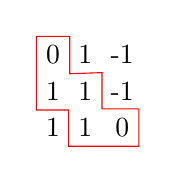
\begin{tikzpicture}
\matrix (m) [matrix of nodes]
{
0 & 1 & -1 \\
1 & 1 & -1 \\
1 & 1 & 0 \\
};
\draw [color=red](m-1-1.north west)--(m-2-1.south west)--(m-2-2.south west)--(m-3-2.south west)--(m-3-3.south east)--(m-3-3.north east)--(m-3-2.north east)--(m-2-2.north east)--(m-1-1.south east)--(m-1-1.north east)--cycle;
\end{tikzpicture}
\end{figure}
If the first round one-way shortest path goes along the red path for getting maximum 3 cherries, it splits the remaining 2 cherries into opposite sides of the diagonal which is impossible for round trip to pick up all cherries. 

Therefore, we have to plan the round trip altogether. Note that the path direction is irrelevant to the problem and we are forced to move only on shortest paths.

We can imagine two persons $p_1$ and $p_2$ are at $(0,0)$ during start. Then they both move by taking different path to $(N-1, N-1)$. After $t$ steps, $p_1$ is in position $(r_1,c_1)$ and $p_2$ in $(r_2, c_2)$. Both positions will have $r_1+c_1=r_2+c_2=t$. Then, $r_2 = r_1 + c_1 - c_2$, which means $r_1,c_1,c_2$ uniquely determine $p_1, p_2$ who have walked the same $t = r_1+c_1$ number of steps. This is suitable for dynamic programming quite nicely.

Suppose $F[r_1][c_1][c_2]$ be the maximum number of cherries obtained by two persons $p_1$ and $p_2$ who are starting at $(r_1, c_1)$ and $(r_2, c_2)$ respectively, and are walking towards $(N-1, N-1)$ by picking up cherries, where $r_2 = r_1+c_1-c_2$.
\par
If $G[r_1][c_1] \neq -1$ and $G[r_2][c_2] \neq -1$, then $F[r_1][c_1][c_2]$ is $(G[r_1][c_1] + G[r_2][c_2])$, plus the maximum of $F[r_1+1][c_1][c_2]$, $F[r_1][c_1+1][c_2]$, $F[r_1+1][c_1][c_2+1]$ and $F[r_1][c_1+1][c_2+1]$. We should also be careful to not double count in case when $p_1$ and $p_2$ are in the same position, i.e., $(r_1, c_1) = (r_2, c_2)$.
\par
Why do we need to plus the 
\[
\max(F[r_1+1][c_1][c_2], F[r_1][c_1+1][c_2], F[r_1+1][c_1][c_2+1], F[r_1][c_1+1][c_2+1])
\]
The reason is these four values corresponds to the 4 possibilities for $p_1$ and $p_2$ moving down and right:
\begin{enumerate}
\item $p_1$ go \textbf{down} and $p_2$ go \textbf{down}: $F[r_1+1][c_1][c_2]$ since $r_2 \gets r_1 + 1 +c_1 -c_2 = (r_1+c_1-c_2) + 1 = r_2+1$
\item $p_1$ go \textbf{right} and $p_2$ go \textbf{down}: $F[r_1][c_1+1][c_2]$ since $r_2 \gets r_1 + c_1 + 1 -c_2 = (r_1+c_1-c_2) + 1 = r_2+1$
\item $p_1$ go \textbf{down} and $p_2$ go \textbf{right}: $F[r_1+1][c_1][c_2+1]$ since $r_2$ is unchanged because $r_2= r_1 + c_1 + 1 -c_2 - 1 = (r_1+c_1-c_2) = r_2$
\item $p_1$ go \textbf{right} and $p_2$ go \textbf{right}: $F[r_1][c_1+1][c_2+1]$ since $r_2$ is unchanged because $r_2= r_1 + c_1 + 1 -c_2 - 1 = (r_1+c_1-c_2) = r_2$
\end{enumerate}

\setcounter{lstlisting}{0}
\begin{lstlisting}[style=customc, caption={Dynamic Programming Top Down}]
int cherryPickup( vector<vector<int>>& grid )
{
    auto N = grid.size();
    vector<vector<vector<int>>> F( N, vector<vector<int>>( N, vector<int>( N, -1 ) ) );
    return ( max )( 0, dfs( grid, F, 0, 0, 0 ) );
}
int dfs( vector<vector<int>>& G, vector<vector<vector<int>>>& memo, size_t r1, size_t c1, size_t c2 )
{
    //r1+c1=r2+c2
    auto r2 = r1 + c1 - c2;
    if( !isValid( G, r1, c1, r2, c2 ) )
    {
        //invalid cell, just return a very small number
        return -99999999;
    }
    //we have value from memo
    if( memo[r1][c1][c2] != -1 )
    {
        return memo[r1][c1][c2];
    }
    auto N = G.size();
    //if person 1 is in the destination cell
    if( ( r1 == N - 1 ) && ( c1 == N - 1 ) )
    {
        return G[N - 1][N - 1];
    }
    //the cherries at (r1,c1)
    int pick = G[r1][c1];

    if( c1 != c2 )
    {
        //(r1,c1) and (r2,c2) are not same cell
        pick += G[r2][c2];
    }
    //get cherries picked from four possible movements
    //combinaton of two players
    //pickFromRR: both persons move right
    int pickFromRR = dfs( G, memo, r1 + 1, c1, c2 );
    //person 1 move right, person 2 move down
    int pickFromRD = dfs( G, memo, r1 + 1, c1, c2 + 1 );
    //person 1 move down, person 2 move right
    int pickFromDR = dfs( G, memo, r1, c1 + 1, c2 );
    //person 1 move down, person 2 move down
    int pickFromDD = dfs( G, memo, r1, c1 + 1, c2 + 1 );
    //get the maximum one from these four movement combinatons
    int pickFromNextMove = ( max )( pickFromRR, pickFromRD );
    pickFromNextMove = ( max )( pickFromDR, pickFromNextMove );
    pickFromNextMove = ( max )( pickFromDD, pickFromNextMove );
    //add to current picked cherries
    pick += pickFromNextMove;
    //save to the memo array
    memo[r1][c1][c2] = pick;
    //return the result
    return pick;
}
//helper function to check if (r1,c1) and (r2,c2) are valid cell or
//they are not throns (-1)
bool isValid( vector<vector<int>>& G, size_t r1, size_t c1, size_t r2, size_t c2 )
{
    auto N = G.size();
    if( ( r1 >= N ) || ( r2 >= N ) || ( c1 >= N ) || ( c2 >= N ) )
    {
        return false;
    }
    if( ( G[r1][c1] == -1 ) || ( G[r2][c2] == -1 ) )
    {
        return false;
    }
    return true;
}
\end{lstlisting}

\subsection{Dynamic Programming Bottom Up}
Like in Top Down approach, Say $r_1 + c_1 = t$ is the $t$-th layer. Since the recursion only references the next layer, we only need to keep two layers in memory at a time.

At time $t$, let $F[r_1][r_2]$ be the most cherries that we can pick up for two people going from $(0, 0)$ to $(r_1, c_1)$ and $(0, 0)$ to $(r_2, c_2)$, where $c_1 = t-r_1$, $c_2 = t-r_2$. 

Since we are evaluating time $t$ from 0 to $N-1+N-1=2N-2$, we will fill $F$ starting from cell $(0,0)$. At time 0, $F[0][0]=G[0][0]$. Next, we loop $t$ from 1 to $2N-2$. Then we will get maximum pickups from four possible positions combinations of the two persons
\begin{itemize}
\item left--left: $p_1$ at $(r_1,c_1-1)$ and $p_2$ at $(r_2, c_2-1)$ which is $F[r_1][r_2]$
\item left--up: $p_1$ at $(r_1,c_1-1)$ and $p_2$ at $(r_2-1, c_2)$ which is $F[r_1][r_2-1]$
\item up--left: $p_1$ at $(r_1-1,c_1)$ and $p_2$ at $(r_2, c_2-1)$ which is $F[r_1-1][r_2]$
\item up--up: $p_1$ at $(r_1-1,c_1)$ and $p_2$ at $(r_2-1, c_2)$ which is $F[r_1-1][r_2-1]$
\end{itemize}

We will use another 2D array as the evaluation result at time $t$ and overwrite to $F$ before moving to next time $t+1$.

\begin{lstlisting}[style=customc, caption={DP Bottom Up}]
int cherryPickup( vector<vector<int>>& grid )
{
    auto N = grid.size();
    //array for DP
    //F[r1][r2] means the maximum cherries picked up
    //when person 1 at (r1,c1) and person 2 at (r2,c2)
    vector<vector<int>> F( N, vector<int>( N, -1 ) );
    //since we iterating time from 0 to 2*N-2
    //we will fill F from (0,0)
    F[0][0] = grid[0][0];
    //The next dp array after evaluating current dp array
    //at time t
    vector<vector<int>> next( N, vector<int>( N, -1 ) );
    for( size_t t = 1; t <= 2 * N - 2; ++t )
    {
        //the range for r1 and r2 could be
        //at time t
        size_t start = 0;
        size_t end = t;
        if( t > N - 1 )
        {
            start = t - ( N - 1 );
            end = N - 1;
        }
        for( size_t r1 = start; r1 <= end; ++r1 )
        {
            for( size_t r2 = start; r2 <= end; ++r2 )
            {
                //get c1 and c2 for two persons
                auto c1 = t - r1;
                auto c2 = t - r2;
                //get cherry amount at (r1,c1) and (r2,c2)
                auto pick1 = grid[r1][c1];
                auto pick2 = grid[r2][c2];
                //reset dp value at these two positions to -1
                next[r1][r2] = -1;
                if( ( pick1 == -1 ) || ( pick2 == -1 ) )
                {
                    //if any person cannot get to the cell, skip
                    continue;
                }
                int cherry = pick1;
                if( r1 != r2 )
                {
                    //two persons are at different cells
                    cherry += pick2;
                }

                //get max picked cherries from last move
                //which could be
                //up-up: (r1-1, c1) and (r2-1, c2)
                //left-up: (r1, c1-1) and (r2-1, c2)
                //up-left: (r1-1, c1) and (r2, c2-1)
                //left-left: (r1, c1-1) and (r2, c2-1)
                //notice F is defined for r1 and r2
                //c1 and c2 are determined from r1 and r2
                int last_pick = F[r1][r2]; //left-left
                if( r1 > 0 )
                {
                    last_pick = ( max )( last_pick, F[r1 - 1][r2] ); // up-left

                }
                if( r2 > 0 )
                {
                    last_pick = ( max )( last_pick, F[r1][r2 - 1] ); // left-up

                }
                if( ( r1 > 0 ) && ( r2 > 0 ) )
                {
                    last_pick = ( max )( last_pick, F[r1 - 1][r2 - 1] ); // up-up
                }
                if( last_pick != -1 )
                {
                    //we can go through last cell to current cell
                    next[r1][r2] = ( max )( next[r1][r2], last_pick + cherry );
                }
            }//end(r2)
        }//end(r1)
        //overwrite F by evaluated dp for current t
        swap( F, next );
    } //end(t)
    return ( max )( 0, F[N - 1][N - 1] );
}
\end{lstlisting}


%\section{742 --- Closest Leaf in a Binary Tree}
Given a binary tree \textbf{where every node has a unique value}, and a target key $k$, find the value of the nearest leaf node to target $k$ in the tree.

Here, nearest to a leaf means the least number of edges traveled on the binary tree to reach any leaf of the tree. Also, a node is called a leaf if it has no children.

In the following examples, the input tree is represented in flattened form row by row. The actual root tree given will be a \fcj{TreeNode} object.

\paragraph{Example 1:}
\begin{flushleft}


\textbf{Input}:

\fcj{root = [1, 3, 2]}, \fcj{k = 1}

Diagram of binary tree:

\begin{figure}[H]
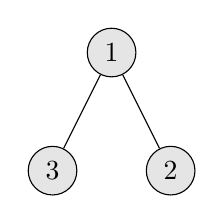
\begin{tikzpicture}
[every node/.style={draw, circle, fill=gray!20!, minimum size=5mm}]
\node{1}
child{node{3}}
child{node{2}};
\end{tikzpicture}
\end{figure}
%          1
%         / \
%        3   2

\textbf{Output}: 2 (or 3)

\textbf{Explanation}: Either 2 or 3 is the nearest leaf node to the target of 1.
\end{flushleft}

\paragraph{Example 2:}
\begin{flushleft}


\textbf{Input}:

\fcj{root = [1], k = 1}

\textbf{Output}: 1


\textbf{Explanation}: The nearest leaf node is the root node itself.
\end{flushleft}

\paragraph{Example 3:}
\begin{flushleft}

\textbf{Input}:

\fcj{root = [1,2,3,4,null,null,null,5,null,6]}, \fcj{k = 2}

Diagram of binary tree:

\begin{figure}[H]
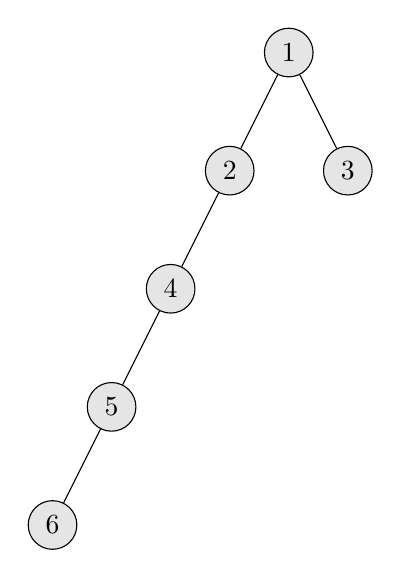
\begin{tikzpicture}
[every node/.style={draw, circle, fill=gray!20!, minimum size=5mm}]
\node{1}
child{node{2} child{node{4} child{node{5} child {node{6}} child[missing]} child[missing]} child[missing]}
child{node{3}};
\end{tikzpicture}
\end{figure}
%             1
%            / \
%           2   3
%          /
%         4
%        /
%       5
%      /
%     6

\textbf{Output}: 3

\textbf{Explanation}: The leaf node with value 3 (and not the leaf node with value 6) is nearest to the node with value 2.
\end{flushleft}

\paragraph{Note:}

\begin{itemize}
\item \fcj{root} represents a binary tree with at least 1 node and at most 1000 nodes.
\item Every node has a unique node.val in range \fcj{[1, 1000]}.
\item There exists some node in the given binary tree for which \fcj{node.val == k}.
\end{itemize}

\subsection{Covert To Graph}
If we can convert the binary tree into a graph, we can use breadth first search to obtain the closest node. In the graph, we do not have the concept of parent and child nodes. Hence, we need to add the parent of current node to its adjacent nodes.

First, we use \textit{DFS} to build the graph from the given tree. Then, we start from those nodes with value equal to $k$ to make \textit{BFS}. In order to avoid go through visited nodes, we make use of a hash set to record nodes we have checked.

\setcounter{lstlisting}{0}
\begin{lstlisting}[style=customc, caption={BFS On Graph Representation Of Binary Tree}]
int findClosestLeaf( TreeNode* root, int k )
{
    //convert tree to adjacent list graph
    unordered_map<TreeNode*, vector<TreeNode*>> g;
    build_graph( g, root, nullptr );
    //find closet leaf node using bfs
    //we need seen to record visited nodes
    queue<TreeNode*> q;
    unordered_set<TreeNode*> seen;
    for( auto const& [node, _] : g )
    {
        if( node->val == k )
        {
            q.push( node );
            seen.insert( node );
        }
    }
    //BFS
    while( !q.empty() )
    {
        auto t = q.front();
        q.pop();

        const auto& adjs = g[t];

        if( adjs.size() == 1 )
        {
            //only leaf node has only one neighbors
            return t->val;
        }
        //find in the adjacent nodes
        for( auto adj : adjs )
        {
            if( seen.find( adj ) == seen.end() )
            {
                seen.insert( adj );
                q.push( adj );
            }
        }
    }
    return k;
}
//helper recursive function to build graph from the binary tree
void build_graph( unordered_map<TreeNode*, vector<TreeNode*>>& G, TreeNode* node, TreeNode* parent )
{
    if( node )
    {
        auto p_node = G.find( node );
        if( p_node == G.end() )
        {
            p_node = G.emplace( node, vector<TreeNode*> {} ).first;
        }
        //add its parent (the parent maybe nullptr for root node)
        p_node->second.push_back( parent );
        if( parent )
        {
            auto p_par = G.find( parent );
            if( p_par == G.end() )
            {
                p_par = G.emplace( parent, vector<TreeNode*> {} ).first;
            }
            p_par->second.push_back( node );
        }
        //recursively build graph for left child
        build_graph( G, node->left, node );
        //recursively build graph for right child
        build_graph( G, node->right, node );
    }
}
\end{lstlisting}

\subsection{Get Distance To The Target Node}
We can make use of \textit{DFS} to find the node with target value. Then the closest leaf to this node must have a \textbf{lowest common ancestor} with the node. Also, this ancestor is on the path from the \fcj{root} to this target node. 

We can get the distances of all ancestors to the target node during \textit{DFS} process via a hash map. Then, we traverse the binary tree. For each node, we check if this node is one of ancestor of the target node through the hash map. If this ancestor is a leaf node, compare against current minimum distance and update result node and minimum distance so far accordingly.

\begin{lstlisting}[style=customc, caption={Get Distances}]
{
    unordered_map<TreeNode*, int> dists;
    //find the ancestor nodes
    //that in the path from root to target node
    find_k( root, k, dists );
    //DFS: get the closest node
    int min_dist = 100000000;
    int ans = k;
    search( root, dists, -1, min_dist, ans );
    return ans;
}
//helper function to find the ancestor nodes from root to the target node
//and get the distance to the target node
int find_k( TreeNode* t, int k, unordered_map<TreeNode*, int>& dists )
{
    //invalid node
    if( !t )
    {
        return -1;
    }
    if( t->val == k )
    {
        //the target node
        dists[t] = 0;
        return 0;
    }
    auto d = find_k( t->left, k, dists );
    if( d != -1 )
    {
        //we find the target node in the left child tree
        //since all nodes have unique values
        //we can return from here
        //1 means the distance from t to t->left
        dists[t] = 1 + d;
        return 1 + d;
    }
    //target node does not exist in the left child tree
    //find in the right child tree
    d = find_k( t->right, k, dists );
    if( d != -1 )
    {
        //1 means the distance from t to t->left
        dists[t] = 1 + d;
        return 1 + d;
    }
    //target node doesn't exist in t's child tree
    return -1;
}
//hepler function to find closest leaf node
void search( TreeNode* t, unordered_map<TreeNode*, int>& dists, int dist, int& min_dist, int& closest )
{
    if( !t )
    {
        return;
    }
    auto p = dists.find( t );
    if( p != dists.end() )
    {
        //get the distance from current node to the target node
        //from the recorded dists
        dist = p->second;
    }
    //check if this node is a leaf node
    if( !t->left && !t->right )
    {
        //check if this leaf node
        //has shortest disance
        //to the target node
        if( dist < min_dist )
        {
            min_dist = dist;
            closest = t->val;
        }

        return;
    }
    //search in the left child tree
    search( t->left, dists, dist + 1, min_dist, closest );
    //search in the right child tree
    search( t->right, dists, dist + 1, min_dist, closest );
}
\end{lstlisting}

%\section{743 --- Network Delay Time}
There are $N$ network nodes, labeled 1 to $N$.

Given \fcj{times}, a list of travel times as directed edges\fcj{ times[i] = (u, v, w)}, where $u$ is the source node, $v$ is the target node, and $w$ is the time it takes for a signal to travel from source to target.

Now, we send a signal from a certain node $K$. How long will it take for all nodes to receive the signal? If it is impossible, return $-1$.

\paragraph{Example 1:}

\begin{flushleft}

\begin{figure}[H]
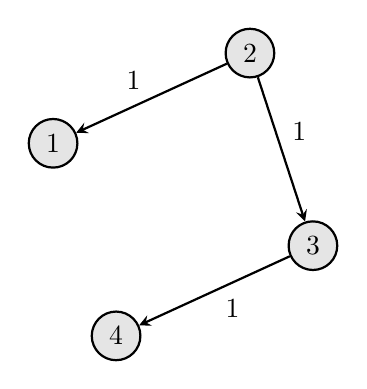
\begin{tikzpicture}
[every node/.style={draw, circle, fill=gray!20!, minimum size=5mm}, >=stealth, ->, thick, auto]
\node(0){2};
\node(1)[below = 5mm of 0, xshift=-25mm]{1};
\node(2)[below = 18mm of 0, xshift=8mm]{3};
\node(3)[below = 5mm of 2, xshift=-25mm]{4};
\draw (0) to node [draw=none,fill=none,swap] {1} (1);
\draw (0) to node [draw=none,fill=none]{1} (2);
\draw (2) to node [draw=none,fill=none]{1} (3);

\end{tikzpicture}
\end{figure}

\textbf{Input}: 

\fcj{times = [[2,1,1],[2,3,1],[3,4,1]]}, $N = 4$, $K = 2$

\textbf{Output}: 2
\end{flushleft}
 

\paragraph{Note:}

\begin{itemize}
\item $N$ will be in the range \fcj{[1, 100]}.
\item $K$ will be in the range $[1, N]$.
\item The length of times will be in the range \fcj{[1, 6000]}.
\item All edges \fcj{times[i] = (u, v, w)} will have $1 \leq u, v \leq N$ and $ 0 \leq w \leq 100$.
\end{itemize}

\subsection{Dijkstra's Algorithm}
The basic idea is that we find the shorted path from $K$ to each node. At the end, the maximum weight of all the nodes will be the answer. Since Dijkstra's algorithm will get shorted path for each node, we only need run once to get the result.

\setcounter{lstlisting}{0}
\begin{lstlisting}[style=customc, caption={Shortest Path}]
int networkDelayTime( vector<vector<int>>& times, int N, int K )
{
    //build adjacent graph from the given edges
    vector<vector<pair<int, int>>> g( N );
    for( const auto& t : times )
    {
        g[t[0] - 1].emplace_back( t[1] - 1, t[2] );
    }
    //delays record each node's shorted path
    //from K
    vector<int> delays( N, -1 );
    //the time to K is zero
    delays[K - 1] = 0;
    //the comparator for the priority queue
    auto cmp = [&delays]( int n1, int n2 )
    {
        return delays[n1] > delays[n2];
    };
    //maximum priority queue (minmum is at the top)
    priority_queue<int, vector<int>, decltype( cmp )> pq( cmp );
    //add start at the beginning
    pq.emplace( K - 1 );
    while( !pq.empty() )
    {
        auto t = pq.top();
        pq.pop();
        if( g[t].empty() )
        {
            continue;
        }
        //find adjacent nodes
        for( const auto& adj : g[t] )
        {
            int w = get<1>( adj );
            int node = get<0>( adj );

            if( delays[node] < 0 )
            {
                //this node has not been visisted
                delays[node] = delays[t] + w;
                pq.emplace( node );
            }
            else if( delays[node]  > delays[t] + w )
            {
                //got shorter path
                delays[node] = delays[t] + w;
                pq.emplace( node );
            }
        }
    }

    //the maximum delay of all the nodes is the answer
    //but we have to check if some nodes are not reached
    //For unreached nodes, their delay is -1
    auto t = minmax_element( begin( delays ), end( delays ) );
    if( *get<0>( t ) < 0 )
    {
        return -1;
    }
    return *get<1>( t );
}
\end{lstlisting}

%\section{744 --- Find Smallest Letter Greater Than Target}
Given a list of sorted characters \fcj{letters} containing only lowercase letters, and given a target letter \fcj{target}, find the smallest element in the list that is larger than the given target.

Letters also wrap around. For example, if the target is \fcj{target = 'z'} and \fcj{letters = ['a', 'b']}, the answer is \fcj{'a'}.


\paragraph{Examples:}
\begin{flushleft}
\textbf{Input}:

\fcj{letters = ["c", "f", "j"]}

\fcj{target = "a"}

\textbf{Output}: \fcj{"c"}

\textbf{Input}:

\fcj{letters = ["c", "f", "j"]}

\fcj{target = "c"}

\textbf{Output}: \fcj{"f"}

\textbf{Input}:

\fcj{letters = ["c", "f", "j"]}

\fcj{target = "d"}

\textbf{Output}: \fcj{"f"}

\textbf{Input}:

\fcj{letters = ["c", "f", "j"]}

\fcj{target = "g"}

\textbf{Output}: \fcj{"j"}

\textbf{Input}:

\fcj{letters = ["c", "f", "j"]}

\fcj{target = "j"}

\textbf{Output}: \fcj{"c"}

\textbf{Input}:

\fcj{letters = ["c", "f", "j"]}

\fcj{target = "k"}

\textbf{Output}: \fcj{"c"}

\end{flushleft}

\paragraph{Note:}

\begin{itemize}
\item \fcj{letters} has a length in range \fcj{[2, 10000]}.
\item \fcj{letters} consists of lowercase letters, and contains at least 2 unique letters.
\item \fcj{target} is a lowercase letter.
\end{itemize}

\subsection{Binary Search}
This is actually a rightmost binary search. If the target letter is larger than all of the letters in the given list, returns the first letter

\setcounter{lstlisting}{0}
\begin{lstlisting}[style=customc, caption={Binary Search}]
char nextGreatestLetter( vector<char>& letters, char target )
{
    size_t l = 0;
    auto r = letters.size();
    while( l < r )
    {
        auto mid = ( l + r ) / 2;
        if( letters[mid] <= target )
        {
            l = mid + 1;
        }
        else
        {
            r = mid;
        }
    }
    if( l == letters.size() )
    {
        l = 0;
    }
    return letters[l];
}
\end{lstlisting}
%\section{745 --- Prefix and Suffix Search}
Given many \fcj{words}, \fcj{words[i]} has weight $i$.

Design a class \fcj{WordFilter} that supports one function, 

\fcj{WordFilter.f(String prefix, String suffix)}. 

It will return the word with given \fcj{prefix} and \fcj{suffix} with maximum weight. If no word exists, return $-1$.

\paragraph{Examples:}

\textbf{Input}:

\begin{flushleft}
\fcj{WordFilter(["apple"])}

\fcj{WordFilter.f("a", "e") // returns 0}

\fcj{WordFilter.f("b", "") // returns -1}

\end{flushleft}
 

\paragraph{Note:}

\begin{itemize}
\item \fcj{words} has length in range \fcj{[1, 15000]}.
\item For each test case, up to \fcj{words.length} queries \fcj{WordFilter.f} may be made.
\item \fcj{words[i]} has length in range \fcj{[1, 10]}.
\item \fcj{prefix}, \fcj{suffix} have lengths in range \fcj{[0, 10]}.
\item \fcj{words[i]} and \fcj{prefix}, \fcj{suffix} queries consist of lowercase letters only.
\end{itemize}

\subsection{Trie of Suffix Wrapped Words}
Consider the word \fcj{'apple'}. For each suffix of the word, we could insert that suffix, followed by \fcj{'#'}, followed by the word, all into the trie.

For example, we will insert \fcj{'#apple'}, \fcj{'e#apple'}, \fcj{'le#apple'}, \fcj{'ple#apple'}, \fcj{'pple#apple'}, \fcj{'apple#apple'} into the trie. Then for a query like \fcj{prefix = "ap"}, \fcj{suffix = "le"}, we can find it by querying the trie tree for \fcj{le#ap}.

We can add each word from the start. Thus, the word with large index will have large weight and it will overwrite corresponding trie nodes' weight correctly. In the end, we just return the recorded weight in the trie node.

\setcounter{lstlisting}{0}
\begin{lstlisting}[style=customc, caption={Suffix Wrapped Words Trie}]
class WordFilter
{
public:
    WordFilter( vector<string>& words )
    {
        m_root = new Trie;
        auto node = m_root;
        int weight = 0;
        for( const auto& word : words )
        {
            //build trie tree
            build_tries( m_root, word, weight );
            ++weight;
        }
    }
    int f( string prefix, string suffix )
    {
        return search( suffix, prefix );
    }

private:
    struct Trie
    {
		//we have 26 lowercase letters
		//and one special letter '#'
        array<Trie*, 27> t_children;
        int t_w;

        Trie()
        {
            t_children.fill( nullptr );
        }
    };
	//build trie tree nodes
	//by appending suffix to the word,
	//spearate by '#'
    void build_tries( Trie* root, string_view word, int weight )
    {
        auto node = root;
		//build '#'+word
        build( root, string_view{}, word, weight );
        for( size_t l = 1; l <= word.size(); ++l )
        {
			//build each suffix of word
			//with ('#' + word)
            build( root, word.substr( word.size() - l, l ), word, weight );
        }

    }
    void build( Trie* root, string_view suffix, string_view word, int weight )
    {
        auto node = root;

        if( !suffix.empty() )
        {
            node = build_helper( node, suffix, weight );
        }
        if( !node->t_children.back() )
        {
            node->t_children.back() = new Trie;
        }
        node = node->t_children.back();
		//larger weight will overwrite smaller weight
        node->t_w = weight;
        build_helper( node, word, weight );
    }
	//build trie helper function
    Trie* build_helper( Trie* node, string_view word, int weight )
    {
        for( auto c :  word )
        {
            auto ci = c - 'a';
            if( !node->t_children[ci] )
            {
                node->t_children[ci] = new Trie;
            }
            node = node->t_children[ci];
            node->t_w = weight;
        }
		//return currently the position of traversing the tree
        return node;
    }
	//search in the trie tree
    int search( string_view suffix, string_view prefix )
    {
        auto node = m_root;
        if( !suffix.empty() )
        {
            node = search_helper( node, suffix );
            if( !node )
            {
                return -1;
            }
        }
		//this is to search node for '#'
        node = node->t_children.back();
        if( !node )
        {
            return -1;
        }
        node = search_helper( node, prefix );
        if( !node )
        {
            return -1;
        }
        return node->t_w;
    }

    Trie* search_helper( Trie* node, string_view word )
    {
        for( auto c : word )
        {
            auto ci = c - 'a';
            if( !node->t_children[ci] )
            {
                return nullptr;
            }

            node = node->t_children[ci];
        }
        return node;
    }
    Trie* m_root;
};
\end{lstlisting}
%\section{746 --- Min Cost Climbing Stairs}
On a staircase, the $i$-th step has some non-negative cost \fcj{cost[i]} assigned (0 indexed).

Once you pay the cost, you can either climb one or two steps. You need to find minimum cost to reach the top of the floor, and you can either start from the step with index 0, or the step with index 1.

\paragraph{Example 1:}

\begin{flushleft}
\textbf{Input}: \fcj{cost = [10, 15, 20]}

\textbf{Output}: 15

Explanation: Cheapest is start on \fcj{cost[1]}, pay that cost and go to the top
\end{flushleft}.

\paragraph{Example 2:}

\begin{flushleft}
\textbf{Input}: \fcj{cost = [1, 100, 1, 1, 1, 100, 1, 1, 100, 1]}

\textbf{Output}: 6

Explanation: Cheapest is start on \fcj{cost[0]}, and only step on 1s, skipping \fcj{cost[3]}.

\end{flushleft}

\paragraph{Note:}

\begin{itemize}
\item \fcj{cost} will have a length in the range \fcj{[2, 1000]}.
\item Every \fcj{cost[i]} will be an integer in the range \fcj{[0, 999]}.

\end{itemize}

\subsection{Dynamic Programming}
There is a clear recursion available: the final cost \fcj{f[i]} to climb the staircase from step $i$ is 

\fcj{f[i] = cost[i] + min(f[i-1], f[i-2])}. 

i.e, either we climb from step $i-1$ by paying cost $f[i-1]$, or we can climb from step $i-2$ by paying cost $f[i-2]$. But to climb from step $i$, we have to add the cost associated which is \fcj{cost[i]}. This motivates dynamic programming.

\setcounter{lstlisting}{0}
\begin{lstlisting}[style=customc, caption={DP}]
int minCostClimbingStairs( vector<int>& cost )
{
    //to climb from step 0
    //we have to pay cost[0]
    int x0 = cost[0];
    //to climb from step 1
    //we have to pay cost[1]
    int x1 = cost[1];
    for( size_t i = 2; i < cost.size(); ++i )
    {
        //to clime from step i
        //we either have climbed from step i-1 by paying cost x1
        //or climbed from step i-2 by paying cost x0
        //then we will pay cost[i] to climb from step i
        int x2 = cost[i] + ( min )( x0, x1 );
        x0 = x1;
        x1 = x2;
    }
    //finally, either we climb from step N-2
    //or climb from step N-1
    //choose the minimum one
    return ( min )( x1, x0 );
}
\end{lstlisting}




%\section{747 --- Largest Number At Least Twice of Others}
In a given integer array \fcj{nums}, there is always exactly one largest element.

Find whether the largest element in the array is at least twice as much as every other number in the array.

If it is, return the \textbf{index} of the largest element, otherwise return $-1$.

\paragraph{Example 1:}

\begin{flushleft}
\textbf{Input}: \fcj{nums = [3, 6, 1, 0]}

\textbf{Output}: 1

\textbf{Explanation}: 6 is the largest integer, and for every other number in the array $x$,
6 is more than twice as big as $x$.  The index of value 6 is 1, so we return 1.

\end{flushleft}
 

\paragraph{Example 2:}

\begin{flushleft}
\textbf{Input}: \fcj{nums = [1, 2, 3, 4]}

\textbf{Output}: $-1$

Explanation: 4 isn't at least as big as twice the value of 3, so we return -1.

\end{flushleft}
 

\paragraph{Note:}

\begin{itemize}
\item \fcj{nums} will have a length in the range \fcj{[1, 50]}.
\item Every \fcj{nums[i]} will be an integer in the range \fcj{[0, 99]}.
\end{itemize}

\subsection{Find Largest And Second Largest Elements}
We can find the largest and second largest elements in \fcj{nums}, and compare them to get the answer.

\setcounter{lstlisting}{0}
\begin{lstlisting}[style=customc, caption={Scan}]
int dominantIndex( vector<int>& nums )
{
    //corner case
    if( nums.size() == 1 )
    {
        return 0;
    }
    //find largest and second largest elements
    int max1 = nums[0];
    int max2 = -1;
    int index = 0;
    int N = static_cast<int>( nums.size() );
    for( int i = 1; i < N; ++i )
    {
        if( nums[i] > max1 )
        {
            index = i;
            max2 = max1;
            max1 = nums[i];
        }
        else if( nums[i] > max2 )
        {
            max2 = nums[i];
        }
    }
    return max1 >= 2 * max2  ? index : -1;
}
\end{lstlisting}
%\section{748 --- Shortest Completing Word}
Find the minimum length word from a given dictionary \fcj{words}, which has all the letters from the string \fcj{licensePlate}. Such a word is said to complete the given string licensePlate

Here, for letters we ignore case. For example, \fcj{"P"} on the \fcj{licensePlate} still matches \fcj{"p"} on the word.

It is guaranteed an answer exists. If there are multiple answers, return the one that occurs first in the array.

The license plate might have the same letter occurring multiple times. For example, given a \fcj{licensePlate} of \fcj{"PP"}, the word \fcj{"pair"} does not complete the licensePlate, but the word \fcj{"supper"} does.

\paragraph{Example 1:}
\begin{flushleft}


\textbf{Input}: 

\fcj{licensePlate = "1s3 PSt"}

\fcj{words = ["step", "steps", "stripe", "stepple"]}

\textbf{Output}: \fcj{"steps"}

\textbf{Explanation}: 

The smallest length word that contains the letters \fcj{"S"}, \fcj{"P"}, \fcj{"S"}, and \fcj{"T"}.

Note that the answer is not \fcj{"step"}, because the letter \fcj{"s"} must occur in the word twice.

Also note that we ignored case for the purposes of comparing whether a letter exists in the word.
\end{flushleft}

\paragraph{Example 2:}
\begin{flushleft}

\textbf{Input}: 

\fcj{licensePlate = "1s3 456"}

\fcj{words = ["looks", "pest", "stew", "show"]}

\textbf{Output}: \fcj{"pest"}

\textbf{Explanation}: 

There are 3 smallest length words that contains the letters \fcj{"s"}.

We return the one that occurred first.
\end{flushleft}

\paragraph{Note:}

\begin{itemize}
\item \fcj{licensePlate} will be a string with length in range \fcj{[1, 7]}.
\item \fcj{licensePlate} will contain digits, spaces, or letters (uppercase or lowercase).
\item \fcj{words} will have a length in the range \fcj{[10, 1000]}.
\item Every \fcj{words[i]} will consist of lowercase letters, and have length in range \fcj{[1, 15]}.
\end{itemize}
%\section{749 --- Contain Virus}
A virus is spreading rapidly, and your task is to quarantine the infected area by installing walls.

The world is modeled as a 2-D array of cells, where 0 represents uninfected cells, and 1 represents cells contaminated with the virus. A wall (and only one wall) can be installed between any two \textbf{4-directionally adjacent cells}, on the shared boundary.

Every night, the virus spreads to all neighboring cells in all four directions unless blocked by a wall. Resources are limited. Each day, you can install walls around only one region -- the affected area (continuous block of infected cells) that threatens the most uninfected cells the following night. There will never be a tie.

Can you save the day? If so, what is the number of walls required? If not, and the world becomes fully infected, return the number of walls used.

\paragraph{Example 1:}

\begin{flushleft}
\textbf{Input}: 

\fcj{grid}:
\[
\begin{bmatrix}
0 & 1 & 0 & 0 & 0 & 0 & 0 & 1\\
0 & 1 & 0 & 0 & 0 & 0 & 0 & 1\\
0 & 0 & 0 & 0 & 0 & 0 & 0 & 1\\
0 & 0 & 0 & 0 & 0 & 0 & 0 & 0
\end{bmatrix}
\]

\textbf{Output}: 10


\textbf{Explanation}:

There are 2 contaminated regions.

On the first day, add 5 walls to quarantine the viral region on the left. The board after the virus spreads is:

\[
\begin{bmatrix}
0 & 1 & 0 & 0 & 0 & 0 & 1 & 1\\
0 & 1 & 0 & 0 & 0 & 0 & 1 & 1\\
0 & 0 & 0 & 0 & 0 & 0 & 1 & 1\\
0 & 0 & 0 & 0 & 0 & 0 & 0 & 1
\end{bmatrix}
\]

On the second day, add 5 walls to quarantine the viral region on the right. The virus is fully contained.
\end{flushleft}

\paragraph{Example 2:}

\begin{flushleft}
\textbf{Input}: 

\fcj{grid}:

\[
\begin{bmatrix}
1 & 1 & 1\\
1 & 0 & 1\\
1 & 1 & 1
\end{bmatrix}
\]

\textbf{Output}: 4

\textbf{Explanation}: 

Even though there is only one cell saved, there are 4 walls built.

Notice that walls are only built on the shared boundary of two different cells.
\end{flushleft}

\paragraph{Example 3:}

\begin{flushleft}
\textbf{Input}: 

\fcj{grid}:

\[
\begin{bmatrix}
1 & 1 & 1 & 0 & 0 & 0 & 0 & 0 & 0\\ 
1 & 0 & 1 & 0 & 1 & 1 & 1 & 1 & 1\\
1 & 1 & 1 & 0 & 0 & 0 & 0 & 0 & 0
\end{bmatrix}
\]

\textbf{Output}: 13

\textbf{Explanation}: 

The region on the left only builds two new walls.
\end{flushleft}

\paragraph{Note:}

\begin{itemize}
\item The number of rows and columns of \fcj{grid} will each be in the range \fcj{[1, 50]}.
\item Each \fcj{grid[i][j]} will be either 0 or 1.
\item Throughout the described process, there is always a contiguous viral region that will infect strictly more uncontaminated squares in the next round.
\end{itemize}
%\section{750 --- Number Of Corner Rectangles}
Given a grid where each entry is only 0 or 1, find the number of corner rectangles.

A \textit{corner rectangle} is 4 distinct 1s on the grid that form an axis-aligned rectangle. Note that only the corners need to have the value 1. Also, all four 1s used must be distinct.
 

\paragraph{Example 1:}

\begin{flushleft}
\textbf{Input}: 

\fcj{grid}:

\[
\begin{bmatrix}
1 & 0 & 0 & 1 & 0 \\
0 & 0 & 1 & 0 & 1 \\
0 & 0 & 0 & 1 & 0 \\
1 & 0 & 1 & 0 & 1
\end{bmatrix}
\] 


\textbf{Output}: 1

\textbf{Explanation}: 

There is only one corner rectangle, with corners \fcj{grid[1][2]}, \fcj{grid[1][4]}, \fcj{grid[3][2]}, \fcj{grid[3][4]}.



\end{flushleft} 

\paragraph{Example 2:}
\begin{flushleft}


\textbf{Input}: 

\fcj{grid}:

\[
\begin{bmatrix}
1 & 1 & 1\\
1 & 1 & 1\\
1 & 1 & 1
\end{bmatrix}
\] 

\textbf{Output}: 9

\textbf{Explanation}: 

There are four $2\times2$ rectangles, four $2\times 3$ and $3\times 2$ rectangles, and one $3\times3$ rectangle.

\end{flushleft} 

\paragraph{Example 3:}

\begin{flushleft}
\textbf{Input}: \fcj{grid = [[1, 1, 1, 1]]}

\textbf{Output}: 0

\textbf{Explanation}: Rectangles must have four distinct corners.

\end{flushleft}
 

\paragraph{Note:}

\begin{itemize}
\item The number of rows and columns of grid will each be in the range \fcj{[1, 200]}.
\item Each \fcj{grid[i][j]} will be either 0 or 1.
\item The number of 1s in the grid will be at most 6000.

\end{itemize}

\subsection{Count Corners}
We ask the question: for each additional row, how many more rectangles are added?

For each pair of 1s in the new row (say at \fcj{new_row[i]} and \fcj{new_row[j]}), we could create more rectangles where that pair forms the base. The number of new rectangles is the number of times some previous row had \fcj{row[i] = row[j] = 1}.

We maintain a count \fcj{count[i, j]}, the number of times we saw \fcj{row[i] = row[j] = 1}. When we process a new row, for every pair \fcj{new_row[i] = new_row[j] = 1}, we add \fcj{count[i, j]} to the answer, then we increment \fcj{count[i, j]}.

\setcounter{lstlisting}{0}
\begin{lstlisting}[style=customc, caption={Count Corners}]
int countCornerRectangles( vector<vector<int>>& grid )
{
    auto N = grid[0].size();
    //count[i,j] is the number of rectangles
    //for a row[i]=row[j]=1
    unordered_map<int, int> count;
    int ans = 0;
    for( const auto& row : grid )
    {
        for( size_t c1 = 0; c1 < N - 1; ++c1 )
        {
            if( row[c1] == 1 )
            {
                for( size_t c2 = c1 + 1; c2 < N; ++c2 )
                {
                    if( row[c2] == 1 )
                    {
                        //get the count of from count[c1, c2]
                        int key = c1 * N + c2;
                        auto it = count.find( key );
                        if( it == count.end() )
                        {
                            //we do not have old_row such that
                            //old_row[c1]=old_row[c2]=1
                            //we add a potential rectangle
                            count.emplace( key, 1 );
                        }
                        else
                        {
                            //we have old_row where
                            //old_row[c1]=old_row[c2]=1
                            //add the number of formed rectanges
                            //to the answer
                            ans += it->second;
                            //increments the formed rectanges at these
                            //two columns because we have a new rectangle
                            //formed with row[c1] and row[c2]
                            ++it->second;
                        }
                    }//end if(row2)
                }//end for(c2)
            }//end if(row1)
        } //end for(c1)
    }//end for (rows)
    return ans;
}
\end{lstlisting}

\subsection{Record Ones Position}
We actually don't need the \fcj{count}. If we found two rows have ones in the same column, we increments the count, say $x$. After scanning a new row, the number of formed rectangles added will be $x\times (x-1)/2$. To speed the process, we can use an array to record the columns 1s in the base row.

\begin{lstlisting}[style=customc, caption={Optimized}]
int countCornerRectangles( vector<vector<int>>& grid )
{
    auto M = grid.size();
    auto N = grid[0].size();
    int ans = 0;
    vector<size_t> ones;
    ones.reserve( N );
    for( size_t r1 = 0;  r1 < M - 1; ++r1 )
    {
        ones.clear();
        //record columns of 1s in row r1
        for( size_t c = 0; c < N; ++c )
        {
            if( grid[r1][c] )
            {
                ones.push_back( c );
            }
        }
        //for any new row r2 after r1
        //check the same columns in ones
        for( size_t r2 = r1 + 1; r2 < M; ++r2 )
        {
            int count = 0;
            for( auto p : ones )
            {
                if( grid[r2][p] )
                {
                    //increment the counter
                    ++count;
                }
            }
            //the new added rectangles will be
            //(count-1)*count/2;
            ans += ( count - 1 ) * count / 2;
        }
    }
    return ans;
}
\end{lstlisting}
%\section{751 --- IP to CIDR}
Given a start IP address \fcj{ip} and a number of ips we need to cover $n$, return a representation of the range as a list (of smallest possible length) of CIDR blocks.

A CIDR block is a string consisting of an IP, followed by a slash, and then the prefix length. For example: \fcj{"123.45.67.89/20"}. That prefix length \fcj{"20"} represents the number of common prefix bits in the specified range.

\paragraph{Example 1:}
\begin{flushleft}

\textbf{Input}: \fcj{ip = "255.0.0.7"}, \fcj{n = 10}

\textbf{Output}: \fcj{["255.0.0.7/32","255.0.0.8/29","255.0.0.16/32"]}

\textbf{Explanation}:

The initial ip address, when converted to binary, looks like this (spaces added for clarity):

\fcj{255.0.0.7 -> 11111111 00000000 00000000 00000111}

The address \fcj{"255.0.0.7/32"} specifies all addresses with a common prefix of 32 bits to the given address, i.e. just this one address.

The address \fcj{"255.0.0.8/29"} specifies all addresses with a common prefix of 29 bits to the given address:

\fcj{255.0.0.8 -> 11111111 00000000 00000000 00001000}

Addresses with common prefix of 29 bits are:

\fcj{11111111 00000000 00000000 00001000}

\fcj{11111111 00000000 00000000 00001001}

\fcj{11111111 00000000 00000000 00001010}

\fcj{11111111 00000000 00000000 00001011}

\fcj{11111111 00000000 00000000 00001100}

\fcj{11111111 00000000 00000000 00001101}

\fcj{11111111 00000000 00000000 00001110}

\fcj{11111111 00000000 00000000 00001111}


The address \fcj{"255.0.0.16/32"} specifies all addresses with a common prefix of 32 bits to the given address, i.e. just 

\fcj{11111111 00000000 00000000 00010000.}

In total, the answer specifies the range of 10 ips starting with the address 255.0.0.7 .

There were other representations, such as:

\fcj{["255.0.0.7/32","255.0.0.8/30", "255.0.0.12/30", "255.0.0.16/32"]},

but our answer was the \textbf{shortest} possible.

Also note that a representation beginning with say, \fcj{"255.0.0.7/30"} would be incorrect,
because it includes addresses like 255.0.0.4 = 11111111 00000000 00000000 00000100 
that are outside the specified range.

\end{flushleft}



\paragraph{Note:}

\begin{enumerate}
\item \fcj{ip} will be a valid IPv4 address.
\item Every implied address \fcj{ip + x} (for $x < n$ ) will be a valid IPv4 address.
\item $n$ will be an integer in the range \fcj{[1, 1000]}.
\end{enumerate}

\subsection{Greedy}

If we know the lowest bit 1, we can know how many addresses a CIDR can cover. The way to find the lowest bit 1 is by using \fcc{x & -x}.

After knowing number of covered ip addresses, we have to take $n$ into consideration. 

\setcounter{lstlisting}{0}
\begin{lstlisting}[style=customc, caption={Greedy}]
vector<string> ipToCIDR( string ip, int n )
{
    //help routint to convert string to integer
    auto to_int = []( string_view s )
    {
        int n = 0;
        for( auto c : s )
        {
            n = n * 10 + ( c - '0' );
        }
        return n;
    };
    //convert ip to integer
    string_view vip( ip );
    size_t start = 0;
    auto p = vip.find( '.', start );
    long long x = 0;
    while( p != string::npos )
    {
        auto sub = vip.substr( start, p - start );
        x = 256 * x + to_int( sub );
        start = p + 1;
        p = vip.find( '.', start );
    }
    x = 256 * x + to_int( vip.substr( start ) );
    //find ranges of ips
    vector<string> ans;
    auto lln = static_cast< long long >( n );
    while( lln > 0 )
    {
        //find how many ips can cover by x
        auto covers = ( x & ( -x ) );
        //make sure covers are less than given n
        while( covers > lln )
        {
            covers >>= 1;
        }
        //change to CIDR
        ans.push_back( toCIDR( x, covers ) );
        x += covers;
        lln -= covers;
    }

    return ans;
}
//get maximum exponent pow so that 2^pow <= covers
long long max_pow2( long long covers )
{
    if( covers == 0 )
    {
        return 1;
    }

    long long pow = 0;

    while( covers > 0 )
    {
        covers >>= 1;
        ++pow;
    }
    return pow - 1;
}
//output to CIDR
string toCIDR( long long x, long long covers )
{
    //change x to ip address
    string ip;
    for( int i = 1; i <= 4; ++i )
    {
        //output each segment
        int y = ( ( x >> ( 32 - i * 8 ) ) & 255 );
        ip += to_string( y );
        ip.push_back( '.' );
    }
    ip.back() = '/';
    //add covers
    auto pow = max_pow2( covers );
    //32-pow is the common prefix length
    ip += to_string( 32LL - pow );
    return ip;
}
\end{lstlisting}

%\section{752 --- Open the Lock}
You have a lock in front of you with 4 circular wheels. Each wheel has 10 slots: \fcj{'0'}, \fcj{'1'}, \fcj{'2'}, \fcj{'3'}, \fcj{'4'}, \fcj{'5'}, \fcj{'6'}, \fcj{'7'}, \fcj{'8'}, \fcj{'9'}. The wheels can rotate freely and wrap around: for example we can turn \fcj{'9'} to be \fcj{'0'}, or \fcj{'0'} to be \fcj{'9'}. Each move consists of turning one wheel one slot.

The lock initially starts at \fcj{'0000'}, a string representing the state of the 4 wheels.

You are given a list of \fcj{deadends} dead ends, meaning if the lock displays any of these codes, the wheels of the lock will stop turning and you will be unable to open it.

Given a \fcj{target} representing the value of the wheels that will unlock the lock, return the minimum total number of turns required to open the lock, or $-1$ if it is impossible.

\paragraph{Example 1:}
\begin{flushleft}


\textbf{Input}: 

\fcj{deadends = ["0201","0101","0102","1212","2002"]}, \fcj{target = "0202"}

\textbf{Output}: 6

\textbf{Explanation}:

A sequence of valid moves would be 

\fcj{"0000" -> "1000" -> "1100" -> "1200" -> "1201" -> "1202" -> "0202"}.

Note that a sequence like \fcj{"0000" -> "0001" -> "0002" -> "0102" -> "0202"} would be invalid, because the wheels of the lock become stuck after the display becomes the dead end \fcj{"0102"}.

\end{flushleft}

\paragraph{Example 2:}

\begin{flushleft}
\textbf{Input}: 

\fcj{deadends = ["8888"]}, \fcj{target = "0009"}

\textbf{Output}: 1

\textbf{Explanation}:

We can turn the last wheel in reverse to move from \fcj{"0000" -> "0009"}.
\end{flushleft}

\paragraph{Example 3:}

\begin{flushleft}
\textbf{Input}: 

\fcj{deadends = ["8887","8889","8878","8898","8788","8988","7888","9888"]}, \fcj{target = "8888"}

\textbf{Output}: $-1$

\textbf{Explanation}:

We can't reach the target without getting stuck.
\end{flushleft}

\paragraph{Example 4:}

\begin{flushleft}
\textbf{Input}: 

\fcj{deadends = ["0000"]}, \fcj{target = "8888"}

\textbf{Output}: $-1$

\end{flushleft}

\paragraph{Note:}

\begin{itemize}
\item The length of \fcj{deadends} will be in the range \fcj{[1, 500]}.
\item \fcj{target} will not be in the list \fcj{deadends}.
\item Every string in \fcj{deadends} and the string \fcj{target} will be a string of 4 digits from the 10,000 possibilities \fcj{'0000'} to \fcj{'9999'}.

\end{itemize}

\subsection{BFS}
The problem is asking for the minimum steps, thus \textit{BFS} can ge the answer quickly. \textit{DFS} would have to traverse all depths to get the answer.

Since the problem has confined the string has four digits, thus we can transform between \fcj{string} and \fcj{integer} to get the memory consumption lower.
\setcounter{lstlisting}{0}
\begin{lstlisting}[style=customc, caption={BFS}]
int openLock( vector<string>& deadends, string target )
{
    //routine to convert to integer
    auto to_int = []( const char* pstr )
    {
        int res = 0;
        for( int i = 0; i < 4; ++i )
        {
            res = res * 10 + ( pstr[i] - '0' );
        }
        return res;
    };
    //record seen integers
    unordered_set<int> dict;
    for( const auto& deadend : deadends )
    {
        int x = to_int( deadend.c_str() );
        if( x == 0 )
        {
            return -1;
        }
        dict.insert( to_int( deadend.c_str() ) );
    }
    queue<int> q;
    q.push( 0 );
    //convert to string with four digits
    auto to_str = []( int i )
    {
        string s = "0000";
        int si = 0;
        while( i )
        {
            int q = i / 10;
            int r = i - 10 * q;
            s[si++] = '0' + r;
            i = q;
        }
        reverse( begin( s ), end( s ) );
        return s;
    };
    int level = 0;
    while( !q.empty() )
    {
        auto sz = q.size();
        for( size_t i = 0; i < sz; ++i )
        {
            auto n = q.front();
            q.pop();
            auto s = to_str( n );
            if( s == target )
            {
                //found target
                //level is the minimum steps
                return level;
            }
            //change each letter in s
            for( int i = 0; i < 4; ++i )
            {
                //increment
                int ci = s[i] - '0';
                int next = ( ci + 1 ) % 10;
                s[i] = '0' + next;
                n = to_int( s.c_str() );
                if( dict.find( n ) == dict.end() )
                {
                    //we have to add now
                    //avoid adding same into the
                    //dict
                    dict.insert( n );
                    q.push( n );
                }
                //decrement
                next = ( ci + 9 ) % 10;
                s[i] = '0' + next;
                n = to_int( s.c_str() );
                if( dict.find( n ) == dict.end() )
                {
                    dict.insert( n );
                    q.push( n );
                }
                //restore s[i]
                s[i] = '0' + ci;
            }
        }
        //increments the steps
        ++level;
    }
    //cannot reach target
    return -1;
}
\end{lstlisting}
%\section{753 --- Cracking the Safe}
There is a box protected by a password. The password is a sequence of $n$ digits where each digit can be one of the first $k$ digits 0, 1, $\ldots$, $k-1$.

While entering a password, the last $n$ digits entered will automatically be matched against the correct password.

For example, assuming the correct password is \fcj{"345"}, if you type \fcj{"012345"}, the box will open because the correct password matches the suffix of the entered password.

Return any password of minimum length that is guaranteed to open the box at some point of entering it.
 

\paragraph{Example 1:}

\begin{flushleft}
\textbf{Input}: 

$n = 1$, $k = 2$

\textbf{Output}: 

\fcj{"01"}

\textbf{Note}: 

\fcj{"10"} will be accepted too.
\end{flushleft}

\paragraph{Example 2:}

\begin{flushleft}
\textbf{Input}: $n = 2$, $k = 2$

\textbf{Output}: \fcj{"00110"}

\textbf{Note}: \fcj{"01100"}, \fcj{"10011"}, \fcj{"11001"} will be accepted too.

\end{flushleft}
 

\paragraph{Note:}

\begin{itemize}
\item $n$ will be in the range \fcj{[1, 4]}.
\item $k$ will be in the range \fcj{[1, 10]}.
\item $k^n$ will be at most 4096.
\end{itemize}

\subsection{Hierholzer's Algorithm}

In order to guarantee to open the box at last, the input password must contain all $n$--length combinations on digits $[0\ldots k-1]$ --- there should be $k^n$ combinations in total.

To make the input password as short as possible, we'd better make each possible $n$--length combination on digits $[0\ldots k-1]$ occurs exactly once as a substring of the password. The existence of such a password is proved by \textit{De Bruijn sequence}:

In combinatorial mathematics, a \textit{de Bruijn sequence} of order $n$ on a size-$k$ alphabet $A$ is a cyclic sequence in which every possible $n$--length string on $A$ occurs exactly once as a substring (i.e., as a contiguous subsequence). 

The \textit{de Bruijn sequences} can be constructed by taking a \textit{Hamiltonian} path of an $n$--dimensional \textit{de Bruijn graph} over $k$ symbols (or equivalently, an \textit{Eulerian cycle} of an $(n − 1)$--dimensional \textit{de Bruijn graph}).

Thus, we can think of this problem as the problem of finding an \textit{Euler} path (a path visiting every edge exactly once) on the following graph: there are $k^{n-1}$ nodes with each node having $k$ edges.

For example, when $k = 4$, $n = 3$, the nodes are \fcj{'00'}, \fcj{'01'}, \fcj{'02'}, $\ldots$, \fcj{'32'}, \fcj{'33'} and each node has 4 edges \fcj{'0'}, \fcj{'1'}, \fcj{'2'}, \fcj{'3'}. A node plus edge represents a complete edge which is a sub-string in our answer.

Any connected directed graph where all nodes have equal in-degree and out-degree has an \textit{Euler circuit} (an \textit{Euler} path ending where it started.) Because our graph is highly connected and symmetric, we should expect intuitively that taking any path greedily in some order will probably result in an Euler path.

This intuition is called \textit{Hierholzer}'s algorithm: whenever there is an \textit{Euler} cycle, we can construct it greedily. The algorithm goes as follows:

\begin{itemize}
\item Choose any starting vertex $v$, and follow a trail of edges from that vertex until returning to $v$. It is not possible to get stuck at any vertex other than $v$, because in-degree and out-degree of every vertex must be same, when the trail enters another vertex $w$ there must be an unused edge leaving $w$.

\item As long as there exists a vertex $u$ that belongs to the current tour but that has adjacent edges not part of the tour, start another trail from $u$, following unused edges until returning to $u$, and join the tour formed in this way to the previous tour.
\end{itemize}

Thus the idea is to keep following unused edges and removing them until we get stuck. Once we get stuck, we back-track to the nearest vertex in our current path that has unused edges, and we repeat the process until all the edges have been used.

For the implementation, We will modify the standard \textit{DFS}: instead of keeping track of nodes, we keep track of (complete) edges: \fcj{seen} records if an edge has been visited.

Also, we need to visit in a way kind of \fcj{"post-order"}, recording the answer after visiting the edge. This is to prevent getting stuck. For example, with $k = 2$, $n = 2$, we have the nodes \fcj{'0'}, \fcj{'1'}. If we greedily visit complete edges \fcj{'00'}, \fcj{'01'}, \fcj{'10'}, we will be stuck at the node \fcj{'0'} prematurely. However, if we visit in post-order, we'll end up visiting \fcj{'00'}, \fcj{'01'}, \fcj{'11'}, \fcj{'10'} correctly.

In general, during the \textit{Hierholzer} walk, we will record the results of other sub-cycles first, before recording the \textit{main} cycle we started from. Technically, we are recording backwards, as we exit the nodes.

\setcounter{lstlisting}{0}
\begin{lstlisting}[style=customc, caption={Hierholzer Algorithm}]
string crackSafe( int n, int k )
{
    //generate start vertex
    string v( n - 1, '0' );
    string ans;
    //this hash set contains all used edges
    unordered_set<string> edges;
    dfs( v, k, edges, ans );
    //add the starting vertex to the path
    ans.append( v.c_str() );
    return ans;
}
//helper function to recursively build Euler path
void dfs( string_view v, int k, unordered_set<string>& edges, string& ans )
{
    for( int ci = 0; ci < k; ++ci )
    {
        //generate one edge from v
        string edge( v.data(), v.size() );
        edge.push_back( '0' + ci );

        if( edges.find( edge ) == edges.end() )
        {
            //this edge is not used
            //add to the set
            edges.emplace( edge );
            //go to next node, which is current edge
            //by removing first letter
            string_view sv_edge( edge );
            dfs( sv_edge.substr( 1 ), k, edges, ans );
            //add current node to the path
            ans.push_back( '0' + ci );
        }
    }
}
\end{lstlisting}

\subsection{Inverse Burrows—Wheeler Transform}
An alternative construction involves concatenating together, in lexicographic order, all the \textit{Lyndon} words whose length divides $n$. An \textit{inverse Burrows—Wheeler transform} can be used to generate the required \textit{Lyndon} words in lexicographic order

%\section{754 --- Reach a Number}
You are standing at position 0 on an infinite number line. There is a goal at position \fcj{target}.

On each move, you can either go left or right. During the $n$--th move (starting from 1), you take $n$ steps.

Return the minimum number of steps required to reach the destination.

Example 1:

\begin{flushleft}
\textbf{Input}: \fcj{target = 3}

\textbf{Output}: 2

\textbf{Explanation}:

On the first move we step from 0 to 1.

On the second step we step from 1 to 3.
\end{flushleft}

\paragraph{Example 2:}

\begin{flushleft}
\textbf{Input}: \fcj{target = 2}

\textbf{Output}: 3

\textbf{Explanation}:

On the first move we step from 0 to 1.

On the second move we step  from 1 to $-1$.

On the third move we step from $-1$ to 2.
\end{flushleft}

\paragraph{Note:}

\begin{itemize}
\item \fcj{target} will be a non-zero integer in the range $[-10^9, 10^9]$.
\end{itemize}

\subsection{Mathematical}
The problem is equivalent to put \fcj{+} and \fcj{-} signs on the numbers 1, 2, 3, $\ldots$, $k$ so that the sum is \fcj{target}.

When \fcj{target < 0}, we can switch the signs of all the numbers to make sure the sum is \fcj{-target}. Thus, the answer for \fcj{target} is the same as \fcj{-target}, and so without loss of generality, we can consider only \fcj{target > 0}.

Suppose $k$ is the smallest number with \fcj{S = 1 + 2 + ... + k >= target}. If \fcj{S == target}, the answer is clearly $k$.

If \fcj{S > target}, we need to change some number signs. If \fcj{delta = S - target} is even, we can always find a subset of \fcj{[1, 2, ..., k]} equal to \fcj{delta / 2} and switch the signs. Thus $S$ will change to \fcj{S - delta/2 - delta/2}, i.e. \fcj{S - delta = target}. so the answer is $k$. (This depends on \fcj{q = delta / 2} being at most $S$.) 

The proof is simple: either $q \leq k$ and we choose it, or we choose $k$ in our subset and try to solve the same instance of the problem for $q = q - k$ and the set \fcj{[1, 2, ..., k-1]}

Otherwise, if \fcj{delta} is \textbf{odd}, we can't do it, as every sign change from positive to negative changes the sum by an \textit{even} number. So let's consider a candidate answer of $k+1$, which change \fcj{delta} to \fcj{delta + k + 1}. If $k$ is odd, then \fcj{delta} is still be odd and we can have an answer of $k+2$. Otherwise, \fcj{delta} will be \textbf{even}, and we will have an answer of $k+1$.

Thus, we subtract \fcj{++k} from \fcj{target} until it goes non-positive. Then $k$ will be as described, and \fcj{target} will be \fcj{delta} as described. We can output the four cases above: 

\begin{enumerate}
\item if \fcj{delta} is \textit{even} then the answer is $k$, 

\item if \fcj{delta} is \textit{odd} then the answer is $k+1$ or $k+2$ depending on $k$ is \textit{even} or \textit{odd}.
\end{enumerate}

\setcounter{lstlisting}{0}
\begin{lstlisting}[style=customc, caption={Mathematical}]
int reachNumber( int target )
{
    int k = 0;
    int S = 0;
    //change target to positive number
    if( target < 0 )
    {
        target = - target;
    }
    //find smallest k such that
    //S=1+2+...+k >= target
    while( S < target )
    {
        ++k;
        S += k;
    }
    int delta = S - target;
    if( delta & 1 )
    {
        //odd
        if( k & 1 )
        {
            //delta+k+2 is even
            return k + 2;
        }
        //delta+k+1 is even
        return k + 1;
    }
    //we can find subset in [1,2,..,k]
    //whose sum is delta/2
    //and change their sign so that the sum
    //is -delta/2. so S is changed to S-delta/2-delta/2
    //=S-delta=target
    return k;
}
\end{lstlisting}
%\section{755 --- Pour Water}
We are given an elevation map, \fcj{heights[i]} representing the height of the terrain at that index. The width at each index is 1. After $ V $ units of water fall at index $K$, how much water is at each index?

Water first drops at index $K$ and rests on top of the highest terrain or water at that index. Then, it flows according to the following rules:

\begin{itemize}
\item If the droplet would eventually fall by moving left, then move left.
\item Otherwise, if the droplet would eventually fall by moving right, then move right.
\item Otherwise, rise at it's current position.
\end{itemize}

Here, \textit{eventually fall} means that the droplet will eventually be at a lower level if it moves in that direction. Also, \textit{level} means the height of the terrain plus any water in that column.

We can assume there's infinitely high terrain on the two sides out of bounds of the array. Also, there could not be partial water being spread out evenly on more than 1 grid block --g- each unit of water has to be in exactly one block.

\paragraph{Example 1:}
\begin{flushleft}
\textbf{Input}: 

\fcj{heights = [2,1,1,2,1,2,2]}, $V = 4$, $K = 3$

\textbf{Output}: \fcj{[2,2,2,3,2,2,2]}

\textbf{Explanation}:
%#       #
%#       #
%##  # ###
%#########
% 0123456    <- index
%
%The first drop of water lands at index K = 3:
%
%#       #
%#   w   #
%##  # ###
%#########
% 0123456    
%
%When moving left or right, the water can only move to the same level or a lower level.
%(By level, we mean the total height of the terrain plus any water in that column.)
%Since moving left will eventually make it fall, it moves left.
%(A droplet "made to fall" means go to a lower height than it was at previously.)
%
%#       #
%#       #
%## w# ###
%#########
% 0123456    
%
%Since moving left will not make it fall, it stays in place.  The next droplet falls:
%
%#       #
%#   w   #
%## w# ###
%#########
% 0123456  
%
%Since the new droplet moving left will eventually make it fall, it moves left.
%Notice that the droplet still preferred to move left,
%even though it could move right (and moving right makes it fall quicker.)
%
%#       #
%#  w    #
%## w# ###
%#########
% 0123456  
%
%#       #
%#       #
%##ww# ###
%#########
% 0123456  
%
%After those steps, the third droplet falls.
%Since moving left would not eventually make it fall, it tries to move right.
%Since moving right would eventually make it fall, it moves right.
%
%#       #
%#   w   #
%##ww# ###
%#########
% 0123456  
%
%#       #
%#       #
%##ww#w###
%#########
% 0123456  
%
%Finally, the fourth droplet falls.
%Since moving left would not eventually make it fall, it tries to move right.
%Since moving right would not eventually make it fall, it stays in place:
%
%#       #
%#   w   #
%##ww#w###
%#########
% 0123456  
%
%The final answer is [2,2,2,3,2,2,2]:
%
%    #    
% ####### 
% ####### 
% 0123456 


\end{flushleft}

\paragraph{Example 2:}

\begin{flushleft}
\textbf{Input}: 

\fcj{heights = [1,2,3,4]}, $V = 2$, $K = 2$

\textbf{Output}: \fcj{[2,3,3,4]}

\textbf{Explanation}:

The last droplet settles at index 1, since moving further left would not cause it to eventually fall to a lower height.

\end{flushleft}


\paragraph{Example 3:}
\begin{flushleft}


\textbf{Input}: 

\fcj{heights = [3,1,3]}, $V = 5$, $K = 1$

\textbf{Output}: \fcj{[4,4,4]}
\end{flushleft}
\paragraph{Note:}

\begin{itemize}
\item \fcj{heights} will have length in \fcj{[1, 100]} and contain integers in \fcj{[0, 99]}.
\item $V$ will be in range \fcj{[0, 2000]}.
\item $K$ will be in range \fcj{[0, heights.length - 1]}.
\end{itemize}

\subsection{Simulation}
When a droplet falls, we check if it is possible for it to fall left, i.e., if \fcj{heights[i - 1] <= heights[i]}. If the condition is met, the water will fall to a \textit{candidate} block in that direction. We keep track of every time we actually fall at index $x$. If we \fcj{"eventually fall"} ($x\neq K$) as described in the problem statement, the unit amount of water will stay there. 

Otherwise, we perform a similar check by going right.

If either left and right cannot drop the water, it will stay in $K$.

\setcounter{lstlisting}{0}
\begin{lstlisting}[style=customc, caption={Simulation}]
vector<int> pourWater( vector<int>& heights, int V, int K )
{
    auto L = static_cast<int>( heights.size() );
    for( int i = 0; i < V; ++i )
    {
        if( ( K > 0 ) && ( heights[K - 1] <= heights[K] ) )
        {
            int fill_p = K;
            //move left
            int l = K;
            //the water can flow left
            //if current height is no larger than its right.
            while( ( l > 0 ) && ( heights[l - 1] <= heights[l] ) )
            {
                if( heights[l - 1] < heights[l] )
                {
                    //the water can only fall into
                    //current index when the height is less than its right
                    fill_p = l - 1;
                    //we cannot break here because maybe some lower block
                    //lie left of current block
                }
                --l;
            }
            if( heights[fill_p] < heights[K] )
            {
                //we found a place that the water
                //eventually fall
                ++heights[fill_p];
                continue;
            }
        }
        if( ( K < L - 1 ) && ( heights[K + 1] <= heights[K] ) )
        {
            //similar check for moving right
            int fill_p = K;
            int r = K;
            //move right
            while( ( r < L - 1 ) && ( heights[r] >= heights[r + 1] ) )
            {
                if( heights[r] > heights[r + 1] )
                {
                    fill_p = r + 1;
                    //similarly, we cannot break here
                    //because some lower block may lie right of current block
                }
                ++r;
            }
            if( heights[fill_p] < heights[K] )
            {
                ++heights[fill_p];
                continue;
            }
        }
        //neither left nor right
        //water will fall
        //stay at K
        ++heights[K];
    }
    return heights;
}
\end{lstlisting}
%\section{756 --- Pyramid Transition Matrix}
We are stacking blocks to form a pyramid. Each block has a color which is a one letter string.

We are allowed to place any color block $C$ on top of two adjacent blocks of colors $A$ and $B$, if and only if $ABC$ is an allowed triple.

We start with a bottom row of \fcj{bottom}, represented as a single string. We also start with a list of allowed triples \fcj{allowed}. Each allowed triple is represented as a string of length 3.

Return \fcj{true} if we can build the pyramid all the way to the top, otherwise \fcj{false}.

\paragraph{Example 1:}

\begin{flushleft}
\textbf{Input}: 

\fcj{bottom = "BCD"}, \fcj{allowed = ["BCG", "CDE", "GEA", "FFF"]}

\textbf{Output}: \fcj{true}

\textbf{Explanation}:

We can stack the pyramid like this:

\begin{figure}[H]
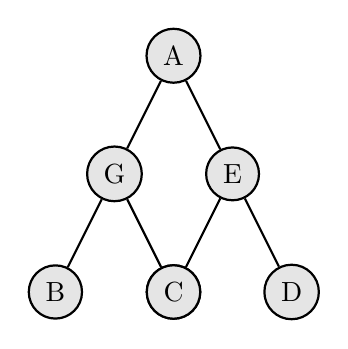
\begin{tikzpicture}
[every node/.style={draw, circle, fill=gray!20!, minimum size=5mm}, thick]
\node{A}
child{node{G} child{node{B}} child{node{C}}}
child{node{E} child{node{C}} child{node{D}}};
\end{tikzpicture}
\end{figure}

%    A
%   / \
%  G   E
% / \ / \
%B   C   D

We are allowed to place $G$ on top of $B$ and $C$ because $BCG$ is an allowed triple.  Similarly, we can place $E$ on top of $C$ and $D$, then $A$ on top of $G$ and $E$.
\end{flushleft}

 

\paragraph{Example 2:}
\begin{flushleft}


\textbf{Input}: \fcj{bottom = "AABA"}, \fcj{allowed = ["AAA", "AAB", "ABA", "ABB", "BAC"]}

\textbf{Output}: \fcj{false}

\textbf{Explanation}:

We can't stack the pyramid to the top.

Note that there could be allowed triples \fcj{(A, B, C)} and \fcj{(A, B, D)} with $C \neq D$.

\end{flushleft} 

\paragraph{Note:}

\begin{itemize}
\item \fcj{bottom} will be a string with length in range \fcj{[2, 8]}.
\item \fcj{allowed} will have length in range \fcj{[0, 200]}.
\item Letters in all strings will be chosen from the set \fcj{['A', 'B', 'C', 'D', 'E', 'F', 'G']}.

\end{itemize}

\subsection{Depth First Search}

\setcounter{lstlisting}{0}
\begin{lstlisting}[style=customc, caption={DFS}]
bool pyramidTransition( string bottom, vector<string>& allowed )
{
    unordered_map<string_view, vector<char>> dict;
    for( const auto& allow :  allowed )
    {
        string_view sv( allow );
        dict[sv.substr( 0, 2 )].push_back( sv.back() );
    }
    unordered_map<string, unsigned char> memo;
    return dfs( bottom, 0, "", dict, memo );
}
bool dfs( string start, size_t index, string next, unordered_map<string_view, vector<char>>& dict, unordered_map<string, unsigned char>& memo )
{
    if( start.size() == 1 )
    {
        return true;
    }
    auto it = memo.find( start );
    if( it != memo.end() )
    {
        return it->second != 0;
    }
    if( next.size() == start.size() - 1 )
    {
        auto res = dfs( next, 0, "", dict, memo );
        memo.emplace( next, res ? 1 : 0 );
        return res;
    }
    string_view sv( start );
    if( index <= start.size() - 2 )
    {
        auto key = sv.substr( index, 2 );
        auto it = dict.find( key );
        if( it == dict.end() )
        {
            return false;
        }
        for( auto c : it->second )
        {
            next.push_back( c );
            if( dfs( start, index + 1, next, dict, memo ) )
            {
                memo.emplace( start, 1 );
                return true;
            }
            next.pop_back();
        }
    }
    return false;
}
\end{lstlisting}
%\section{757 --- Set Intersection Size At Least Two}
An integer interval \fcj{[a, b]} (for integers $a < b$) is a set of all consecutive integers from $a$ to $b$, including $a$ and $b$.

Find the minimum size of a set $S$ such that for every integer interval $A$ in intervals, the intersection of $S$ with $A$ has size at least 2.

\paragraph{Example 1:}

\begin{flushleft}
\textbf{Input}: \fcj{intervals = [[1, 3], [1, 4], [2, 5], [3, 5]]}

\textbf{Output}: 3

\textbf{Explanation}:

Consider the set \fcj{S = {2, 3, 4}}.  For each interval, there are at least 2 elements from S in the interval.

Also, there isn't a smaller size set that fulfills the above condition.

Thus, we output the size of this set, which is 3.
\end{flushleft}

\paragraph{Example 2:}

\begin{flushleft}
\textbf{Input}: \fcj{intervals = [[1, 2], [2, 3], [2, 4], [4, 5]]}

\textbf{Output}: 5

\textbf{Explanation}:

An example of a minimum sized set is \fcj{[1, 2, 3, 4, 5]}.
\end{flushleft}

\paragraph{Note:}

\begin{itemize}
\item \fcj{intervals} will have length in range \fcj{[1, 3000]}.
\item \fcj{intervals[i]} will have length 2, representing some integer interval.
\item \fcj{intervals[i][j]} will be an integer in $ [0, 10^8] $.
\end{itemize}

\subsection{Greedy}
For greedy algorithm to work, we want to work with smaller intervals first. This is obvious: if interval $b$ completely contains interval $a$ and our set $S$ has two same numbers as in $a$, there must be two same numbers in $b$.

To be more efficient, we need the intervals to be sorted. Since we want to process shorter interval first, we will sort the intervals per the ending position by ascending order. If two intervals have same ending positions, the one with larger starting position is put in front. 

Then, there are three cases regarding the relationship of current interval and the set $S$ 
\begin{enumerate}
\item No intersection. We will fetch two numbers from current interval to add to $S$. To minimize the size of $S$, we shall choose the two maximum numbers of current interval. By this way, the probability that $S$ has intersection with intervals after is high.
\item Intersection with one number. This number must be the starting one of current interval. We need to get another number to add to $S$. By the similar analysis as before, this number to be added to $S$ must be the maximum number of current interval (or the ending one of current interval).
\item Intersection with two or more than two numbers. In this case, just skip current interval.
\end{enumerate}

In the implementation, we maintain an array $A$ to represent $S$. At start, we put two $-1$s into $A$. During traversing the sorted intervals, 

\begin{itemize}
\item If current one's starting number is less than the second to last in $A$, this is the case 3.
\item If current one's starting number is larger than the last number in $A$, this is the case 1.
\item Otherwise, this is the case 2.
\end{itemize}

Finally, we subtract 2 from the length of $A$ to remove the effect of two $-1$s.

\setcounter{lstlisting}{0}
\begin{lstlisting}[style=customc, caption={Greedy}]
int intersectionSizeTwo( vector<vector<int>>& intervals )
{
    //sort intervals with ending number by ascending order
    //and larger starting number when ending numbers are equal
    sort( begin( intervals ), end( intervals ), []( const vector<int>& itv1, const vector<int>& itv2 )
    {
        if( itv1[1] < itv2[1] )
        {
            return true;
        }
        if( itv1[1] == itv2[1] )
        {
            return itv1[0] > itv2[0];
        }

        return false;
    } );
    //the minimum size set
    vector<int> S{-1, -1};
    for( const auto& i : intervals )
    {
        if( i[0] <= S[S.size() - 2] )
        {
            //intersection with two or more numbers
            //skip
        }
        else if( i[0] > S.back() )
        {
            //no intersection
            //add maximum two numbers of current interval
            S.push_back( i[1] - 1 );
            S.push_back( i[1] );
        }
        else
        {
            //only one number in intersection
            S.push_back( i[1] );
        }
    }
    //substract 2 which is the effect of two -1s
    return static_cast<int>( S.size() ) - 2;
}
\end{lstlisting}

\subsection{Constant Space}
Notice in the last approach, we only need the maximum and the second to maximum numbers. Thus, we can reduce the memory consumption to $O(1)$.

\begin{lstlisting}[style=customc, caption={Constant Space}]
int intersectionSizeTwo( vector<vector<int>>& intervals )
{
    sort( begin( intervals ), end( intervals ), []( const vector<int>& itv1, const vector<int>& itv2 )
    {
        if( itv1[1] < itv2[1] )
        {
            return true;
        }
        if( itv1[1] == itv2[1] )
        {
            return itv1[0] > itv2[0];
        }

        return false;
    } );
    //the maximum number in the set S
    int max1 = -1;
    //the second to maximum number in the set S
    int max2 = -1;
    //the size of the set S
    int best_size = 0;
    for( const auto& i : intervals )
    {
        if( i[0] <= max2 )
        {
            //intersection with >=2 numbers
            continue;
        }
        else if( i[0] > max1 )
        {
            //no intersection
            //add maximum 2 numbers of interval i
            //to set S
            best_size += 2;
            max1 = i[1];
            max2 = max1 - 1;
        }
        else
        {
            //intersection with 1 number
            //which is i[0]
            //add i[1] to S
            ++best_size;
            max2 = max1;
            max1 = i[1];
        }
    }
    return best_size;
}
\end{lstlisting}
%\section{758 --- Bold Words in String}

Given a set of keywords \fcj{words} and a string $S$, make all appearances of all keywords in $S$ bold. Any letters between \fcj{<b>} and \fcj{</b>} tags become bold.

The returned string should use the least number of tags possible, and of course the tags should form a valid combination.

For example, given that \fcj{words = ["ab", "bc"]} and \fcj{S = "aabcd"}, we should return \fcj{"a<b>abc</b>d"}. Note that returning \fcj{"a<b>a<b>b</b>c</b>d"} would use more tags, so it is incorrect.

\paragraph{Note:}

\begin{enumerate}
\item \fcj{words} has length in range \fcj{[0, 50]}.
\item \fcj{words[i]} has length in range \fcj{[1, 10]}.
\item $S$ has length in range \fcj{[0, 500]}.
\item All characters in \fcj{words[i]} and $S$ are lowercase letters.
\end{enumerate}

\subsection{Brute Force}
We check for all occurrences of each word and mark the corresponding letters bold.

We maintain a boolean array \fcj{flags} and \fcj{flags[i] = true} if and only if the $i$-th letter is bold. For each starting position $i$ in $S$, and for each word, if \fcj{S[i]} starts with this word, we set the appropriate letters in $S$ as bold.

With generated \fcj{flags}, a letter in position $i$ is 

\begin{itemize}
\item the first bold letter of the group if \fcc{flags[i] && (i == 0 \|\| flags[i-1]==0)}, 
\item and is the last bold letter if \fcc{flags[i] && (i == N-1 \|\| flags[i+1]==0)}. 

\end{itemize}
Once we know which letters are the first and last bold letters of a group, we know where to put the \fcj{"<b>"} and \fcj{"</b>"} tags.

\setcounter{lstlisting}{0}
\begin{lstlisting}[style=customc, caption={Brute Force}]
string boldWords( vector<string>& words, string S )
{
    vector<unsigned char> flags( S.size(), 0 );
    string_view sv( S );
    for( size_t i = 0; i < S.size(); ++i )
    {
        for( const auto& word : words )
        {
            string_view svw( word );
            if( sv.substr( i, word.size() ) == svw )
            {
                //sv[i...i+word.size()-1]=word
                //mark flags[i,i+word.size()-1]
                //as bold letter flag
                auto b = flags.begin();
                advance( b, i );
                auto e = b;
                advance( e, word.size() );
                fill( b, e, 1 );
            }
        }
    }
    string ans;
    for( size_t i = 0; i < S.size(); ++i )
    {
        if( ( flags[i] == 1 ) && ( ( i == 0 ) || ( flags[i - 1] == 0 ) ) )
        {
            //the start of bold letter
            ans += "<b>";
        }
        ans.push_back( S[i] );
        if( ( flags[i] == 1 ) && ( ( i == ( S.size() - 1 ) ) || ( flags[i + 1] == 0 ) ) )
        {
            //the end of bold letter
            ans += "</b>";
        }
    }
    return ans;
}
\end{lstlisting}
%\section{759 --- Employee Free Time}
We are given a list \fcj{schedule} of employees, which represents the working time for each employee.

Each employee has a list of non-overlapping \fcj{Intervals}, and these intervals are in sorted order.

Return the list of finite intervals representing \textbf{common}, \textbf{positive-length free time} for \textit{all} employees, also in sorted order.

\paragraph{Example 1:}

\begin{flushleft}
\textbf{Input}: \fcj{schedule = [[[1,2],[5,6]],[[1,3]],[[4,10]]]}

\textbf{Output}: \fcj{[[3,4]]}

\textbf{Explanation}:

There are a total of three employees, and all common

free time intervals would be $[-\infty, 1]$, $[3, 4]$, $[10, \infty]$.

We discard any intervals that contain inf as they aren't finite.
\end{flushleft}

 

\paragraph{Example 2:}

\begin{flushleft}
\textbf{Input}: \fcj{schedule = [[[1,3],[6,7]],[[2,4]],[[2,5],[9,12]]]}

\textbf{Output}: \fcj{[[5,6],[7,9]]}
\end{flushleft}

 
Even though we are representing \fcj{Intervals} in the form \fcj{[x, y]}, the objects inside are \fcj{Intervals}, not lists or arrays. 

For example, \fcj{schedule[0][0].start = 1}, \fcj{schedule[0][0].end = 2}, and \fcj{schedule[0][0][0]} is not defined.


Also, we wouldn't include intervals like \fcj{[5, 5]} in our answer, as they have zero length.

\paragraph{Note:}

\begin{itemize}
\item \fcj{schedule} and \fcj{schedule[i]} are lists with lengths in range \fcj{[1, 50]}.
\item \fcj{0 <= schedule[i].start < schedule[i].end <=} $10^8$.
\end{itemize}

\subsection{Line Sweep}
Sort the input intervals per the starting time, and find overlapped intervals

\setcounter{lstlisting}{0}
\begin{lstlisting}[style=customc, caption={Line Sweep}]

vector<Interval*> employeeFreeTime( vector<vector<Interval*>> schedule )
{
    //group the intervals together
    vector<Interval*> schs;
    for( const auto& itvs : schedule )
    {
        schs.insert( schs.end(), begin( itvs ), end( itvs ) );
    }
    //sort the intervals per the start time first
    //end the end time when two have equal start times
    sort( begin( schs ), end( schs ), []( Interval * p1, Interval * p2 )
    {

        if( p1->start < p2->start )
        {
            return true;
        }
        if( p1->start == p2->start )
        {
            return p1->end < p2->end;
        }
        return false;
    } );
    vector<Interval*> ans;
    //find overlapped intervals
    auto overlap = schs[0];
    for( size_t i = 1; i < schs.size(); ++i )
    {
        if( overlap->end >= schs[i]->start )
        {
            //overlap with current merged interval
            overlap->end = ( max )( overlap->end, schs[i]->end );
        }
        else
        {
            //we found a non-overlap interval
            //add to the output
            ans.emplace_back( new Interval( overlap->end, schs[i]->start ) );
            overlap = schs[i];
        }
    }
    return ans;
}
\end{lstlisting}

\subsection{Boundary Count}
Similar to problem \textbf{731 --- My Calendar II}, When booking a new interval \fcj{[start, end]}, use a tree map \fcj{delta} to count as  \fcj{delta[start]++} and \fcj{delta[end]--}.

When processing the values of \fcj{delta} in sorted order of their keys, the running sum active is the number of overlapped intervals at that time. If the sum is zero, we are at the end of a group of overlapped intervals, or the start of free time range, say $x$. 

We add \fcj{[x,-1]} into the output list where $-1$ means we have not updated the end of free time range. This end will be updated by the next interval's start time.

Finally, we may add an interval which has $-1$ as the end time. We will remove it at the end.

\begin{lstlisting}[style=customc, caption={Boundry Count}]
vector<Interval*> employeeFreeTime( vector<vector<Interval*>> schedule )
{
    //used for booking intervals
    map<int, int> events;
    for( const auto& itvs : schedule )
    {
        for( auto p : itvs )
        {
            //start: increment count
            events[p->start] += 1;
            //end: decrement count
            events[p->end] -= 1;
        }
    }
    //go through the boundry counts
    int count = 0;
    vector<Interval*> ans;
    for( const auto& evt : events )
    {
        count += get<1>( evt );
        if( count == 0 )
        {
            //we are at the end of a group of overlapped intervals
            //or the start of a free time range
            ans.push_back( new Interval( get<0>( evt ), -1 ) );
        }
        else
        {
            if( !ans.empty() && ( ans.back()->end < 0 ) )
            {
                //update the last added free time range end
                //which is current interval's start time
                ans.back()->end = get<0>( evt );
            }
        }
    }
    //finally, we will remove last one we added
    //because this one has -1 as the end time.
    if( !ans.empty() )
    {
        ans.pop_back();
    }
    return ans;
}
\end{lstlisting}
%\include{760}
%\section{761 --- Special Binary String}
Special binary strings are binary strings with the following two properties:

\begin{itemize}
\item The number of 0s is equal to the number of 1s.
\item Every prefix of the binary string has at least as many 1s as 0s.
\end{itemize}

Given a special string $S$, a move consists of choosing two consecutive, non-empty, special substrings of $S$, and swapping them. (Two strings are consecutive if the last character of the first string is exactly one index before the first character of the second string.)

At the end of any number of moves, what is the lexicographically largest resulting string possible?

\paragraph{Example 1:}

\begin{flushleft}
\textbf{Input}: \fcj{S = "11011000"}

\textbf{Output}: \fcj{"11100100"}

\textbf{Explanation}:

The strings \fcj{"10"} (occuring at \fcj{S[1]}) and \fcj{"1100"} (at \fcj{S[3]}) are swapped.

This is the lexicographically largest string possible after some number of swaps.
\end{flushleft}

\paragraph{Note:}

\begin{itemize}
\item $S$ has length at most 50.
\item $S$ is guaranteed to be a special binary string as defined above.
\end{itemize}

\subsection{DFS}
If we regard 1, 0 in the definition of the special string as \fcj{'('} and \fcj{')'} separately,

the problem is actually to get the string which is so-called valid parenthesis and meanwhile is the lexicographically largest.

It is intuitive that we prefer deeper valid parenthesis to be in front (\textbf{deeper} means the string surrounded with more pairs of parenthesis, e.g., \fcj{'(())'} is deeper than \fcj{'()'} ). We can achieve that by sorting them reversely.

we go through $S$. Whenever the parentheses we met can be balanced, we construct valid parentheses by putting \fcj{'('} on the left boundary, \fcj{')'} on the right boundary, and doing with the inner part following the same pattern.

\setcounter{lstlisting}{0}
\begin{lstlisting}[style=customc, caption={DFS}]
string makeLargestSpecial( string S )
{
    size_t start = 0;
    vector<string> segs;
    int bal = 0;
    for( size_t i = 0; i < S.size(); ++i )
    {
        bal += ( S[i] == '0' ) ? -1 : 1;
        if( bal == 0 )
        {
            //this special string can be rearranged recursively
            //add to the array
            segs.push_back( "1" + makeLargestSpecial( S.substr( start + 1, i - start - 1 ) ) + "0" );
            //the next special string start at i+1
            start = i + 1;
        }
    }
    //sort generated largest special strings
    sort( segs.begin(), segs.end() );
    string init;
    //add the string from end to beginning
    return accumulate( rbegin( segs ), rend( segs ), init );
}
\end{lstlisting}
\section{771. Jewels and Stones}
You're given strings \fcj{J} representing the types of stones that are jewels, and \fcj{S} representing the stones you have.  Each character in \fcj{S} is a type of stone you have.  You want to know how many of the stones you have are also jewels.

The letters in \fcj{J} are guaranteed distinct, and all characters in \fcj{J} and \fcj{S} are letters. Letters are case sensitive, so \fcj{"a"} is considered a different type of stone from \fcj{"A"}.

\paragraph{Example 1:}

\begin{flushleft}
\textbf{Input}: \fcj{J = "aA"}, \fcj{S = "aAAbbbb"}

\textbf{Output}: 3
\end{flushleft}

\paragraph{Example 2:}

\begin{flushleft}
\textbf{Input}: \fcj{J = "z"}, \fcj{S = "ZZ"}

\textbf{Output}: 0
\end{flushleft}

\paragraph{Note:}

\begin{itemize}
\item \fcj{S} and \fcj{J} will consist of letters and have length at most 50.

\item The characters in \fcj{J} are distinct.
\end{itemize}

\subsection{Hash Set}
\textbf{Easy} Problem. Simulate hash set by an array

\setcounter{lstlisting}{0}
\begin{lstlisting}[style=customc, caption={Hash Set}]
int numJewelsInStones( string J, string S )
{
    array<int, 52> m;
    m.fill( 0 );
    //1. add letters in J to a hash set
    for( auto c : J )
    {
        if( ( c <= 'Z' ) && ( c >= 'A' ) )
        {
            m[c - 'A'] = 1;
        }
        else
        {
            m[c - 'a' + 26] = 1;
        }
    }
    //2. check each letter in S against the hash set
    int ans = 0;
    for( auto c : S )
    {
        if( ( c <= 'Z' ) && ( c >= 'A' ) )
        {
            ans += m[c - 'A'];
        }
        else
        {
            ans += m[c - 'a' + 26];
        }
    }
    return ans;
}
\end{lstlisting}
\section{772 --- Basic Calculator III}
Implement a basic calculator to evaluate a simple expression string.

The expression string may contain open \fcj{(} and closing parentheses \fcj{)}, the plus \fcj{+} or minus sign \fcj{-}, non-negative integers and empty spaces .

The integer division should truncate toward zero.

You may assume that the given expression is always valid. All intermediate results will be in the range of \fcj{[-2147483648, 2147483647]}.

Some examples:

\fcj{"1 + 1" = 2}

\fcj{" 6-4 / 2 " = 4}

\fcj{"2*(5+5*2)/3+(6/2+8)" = 21}

\fcj{"(2+6* 3+5- (3*14/7+2)*5)+3"=-12}

\subsection{Brute Force}
To process the parenthesis, we maintain a variable \fcj{balance}. Whenever we find a \fcj{"("}, start the process by increment \fcj{balance} for \fcj{"("}, and decrement for \fcj{")"}. When \fcj{balance} becomes zero, we recursively process the substring between \fcj{"("} and \fcj{")"}.

\setcounter{lstlisting}{0}
\begin{lstlisting}[style=customc, caption={Brute Force}]
int calculate( string s )
{
    return evaluate( s );
}
//helper function to evaluate the exprssion
int evaluate( string_view expr )
{
    auto L = expr.size();
    long long parse_num = 0;
    long long cur_res = 0;
    long long res = 0;
    //trick: initialize op as +
    //can simply the expression evaluation
    char op = '+';
    for( size_t i = 0; i < L; ++i )
    {
        auto c = expr[i];
        if( ( c >= '0' ) && ( c <= '9' ) )
        {
            //string to integer
            parse_num = parse_num * 10 + ( c - '0' );
        }
        else if( c == '(' )
        {
            //using balance to find
            //substring between a pair of
            //parenthesis
            auto j = i + 1;
            int balance = 1;
            for( ; j < L; ++j )
            {
                if( expr[j] == '(' )
                {
                    ++balance;
                }
                else if( expr[j] == ')' )
                {
                    --balance;
                }

                if( balance == 0 )
                {
                    break;
                }
            }
            parse_num = evaluate( expr.substr( i + 1, j - i - 1 ) );
            i = j;
        }
        //we cannot use "else if" here
        //since we have to use parse_num as early as possible
        //3. process the operator and number so far
        if( ( c == '+' ) || ( c == '-' ) || ( c == '*' ) || ( c == '/' ) || ( i == L - 1 ) )
        {
            //check last operator
            //and perform the computation
            switch( op )
            {
            case '+':
                cur_res += parse_num;
                break;
            case '-':
                cur_res -= parse_num;
                break;
            case '*':
                cur_res *= parse_num;
                break;
            case '/':
                cur_res /= parse_num;
                break;
            }
            if( ( c == '+' ) || ( c == '-' ) || ( i == L - 1 ) )
            {
                //if current operator is +/-
                //we accumulate the result of cur_res
                //also for i=L-1
                res += cur_res;
                //reset the result obtained so far
                cur_res = 0;
            }
            //update last operator
            op = c;
            //reset parsed number
            parse_num = 0;
        }
    }
    return res;
}
\end{lstlisting}
\section{773 --- Sliding Puzzle}
On a $2\times 3$ \fcj{board}, there are 5 tiles represented by the integers 1 through 5, and an empty square represented by 0.

A move consists of choosing 0 and a 4-directionally adjacent number and swapping it.

The state of the board is \textit{solved} if and only if the \fcj{board} is \fcj{[[1,2,3],[4,5,0]]}.

Given a puzzle board, return the least number of moves required so that the state of the board is solved. If it is impossible for the state of the board to be solved, return $-1$.

\paragraph{Examples:}
\begin{flushleft}


\textbf{Input}: \fcj{board = [[1,2,3],[4,0,5]]}

\textbf{Output}: 1

\textbf{Explanation}: Swap the 0 and the 5 in one move.

\textbf{Input}: \fcj{board = [[1,2,3],[5,4,0]]}

\textbf{Output}: $-1$

\textbf{Explanation}: No number of moves will make the board solved.

\textbf{Input}: \fcj{board = [[4,1,2],[5,0,3]]}

\textbf{Output}: 5

\textbf{Explanation}: 5 is the smallest number of moves that solves the board.

An example path:

After move 0: \fcj{[[4,1,2],[5,0,3]]}

After move 1: \fcj{[[4,1,2],[0,5,3]]}

After move 2: \fcj{[[0,1,2],[4,5,3]]}

After move 3: \fcj{[[1,0,2],[4,5,3]]}

After move 4: \fcj{[[1,2,0],[4,5,3]]}

After move 5: \fcj{[[1,2,3],[4,5,0]]}

\textbf{Input}: \fcj{board = [[3,2,4],[1,5,0]]}

\textbf{Output}: 14

\end{flushleft}

\paragraph{Note:}

\begin{itemize}
\item \fcj{board} will be a $2 \times 3$ array as described above.
\item \fcj{board[i][j]} will be a permutation of \fcj{[0, 1, 2, 3, 4, 5]}.
\end{itemize}

\subsection{BFS}
We can think of this problem as a shortest path problem on a graph. Each node is a different board state, and we connect two boards by an edge if they can be transformed into one another in one move. We can solve shortest path problems with \textit{breadth first search}.

\setcounter{lstlisting}{0}
\begin{lstlisting}[style=customc, caption={BFS}]
int slidingPuzzle( vector<vector<int>>& board )
{
    pair<int, int> p_zero;
    //transform board to integer
    auto get_key = [&board]( pair<int, int>& p_zero )
    {
        int key = 0;
        for( int r = 0; r < 2; ++r )
        {
            for( int c = 0; c < 3; ++c )
            {
                if( board[r][c] == 0 )
                {
                    get<0>( p_zero ) = r;
                    get<1>( p_zero ) = c;
                }

                key = key * 10 + board[r][c];
            }
        }
        return key;
    };
    //transform integer to the board
    auto to_board = []( int n, vector<vector<int>>& board )
    {
        for( int r = 1; r >= 0; --r )
        {
            for( int c = 2; c >= 0; --c )
            {
                int q = n / 10;
                board[r][c] = n - 10 * q;
                n = q;
            }
        }
    };
    int target = 123450;
    unordered_set<int> seen;
    //start BFS
    queue<array<int, 3>> q;
    auto key = get_key( p_zero );
    //each element in the queue
    //has key, and (r,c) of zero element
    q.emplace( array<int, 3> {key, get<0>( p_zero ), get<1>( p_zero )} );
    seen.insert( key );
    //the breadth level
    int level = 0;
    vector<pair<int, int>> dirs = {{-1, 0}, {1, 0}, {0, 1}, {0, -1}};
    while( !q.empty() )
    {
        auto level_sz = q.size();
        for( size_t i = 0; i < level_sz; ++i )
        {
            auto t = q.front();
            q.pop();
            if( t[0] == target )
            {
                return level;
            }
            //get (r,c) of zero
            auto r = t[1];
            auto c = t[2];
            to_board( t[0], board );
            //find 4 adjacent elements to swap
            for( int di = 0; di < 4; ++di )
            {
                auto[dr, dc] = dirs[di];
                auto nr = r + dr;
                auto nc = c  + dc;
                if( ( nr >= 0 ) && ( nr < 2 ) && ( nc >= 0 ) && ( nc < 3 ) )
                {
                    //swap zero with board[nr][nc]
                    swap( board[nr][nc], board[r][c] );
                    key = get_key( p_zero );
                    if( seen.find( key ) == seen.end() )
                    {
                        q.emplace( array<int, 3> {key, get<0>( p_zero ), get<1>( p_zero )} );
                        //add key to hash set
                        seen.insert( key );
                    }
                    //restore board before swap
                    swap( board[nr][nc], board[r][c] );
                }
            } //end direction
        }//end for level
        ++level;
    }//end while q
    return -1;
}
\end{lstlisting}
\section{774 --- Minimize Max Distance to Gas Station}
On a horizontal number line, we have gas stations at positions \fcj{stations[0]}, \fcj{stations[1]}, $\ldots$, \fcj{stations[N-1]}, where \fcj{N = stations.length}.

Now, we add $K$ more gas stations so that \textbf{D}, the maximum distance between adjacent gas stations, is minimized.

Return the smallest possible value of \textbf{D}.

\paragraph{Example:}

\begin{flushleft}
\textbf{Input}: 

\fcj{stations = [1, 2, 3, 4, 5, 6, 7, 8, 9, 10]}

$K = 9$

\textbf{Output}: \fcj{0.500000}
\end{flushleft}

\paragraph{Note:}

\begin{itemize}
\item \fcj{stations.length} will be an integer in range \fcj{[10, 2000]}.
\item \fcj{stations[i]} will be an integer in range $[0, 10^8]$.
\item $K$ will be an integer in range $[1, 10^6]$.
\item Answers within $10^{-6}$ of the true value will be accepted as correct.
\end{itemize}

\subsection{Dynamic Programming [MLE]}
Suppose \fcj{F[n][y]} be the answer by adding \fcj{y} more gas stations to the first \fcj{n} intervals of stations, where the $i$--th interval is \fcj{dist[i] = stations[i+1] - stations[i]}. 

To get \fcj{F[n+1][y]}, we can test by putting $x$ gas stations in the $(n+1)$--th interval to get a best distance as \fcj{dist[n+1]/(x+1)}. The the best distance for the rest of the intervals is \fcj{dist[n][y-x]}. Then, \fcj{F[n+1][t]} is the minimum when we try every possible $x$ from 0 to $y$.

Finally, The last element of \fcj{F} is the answer.

\setcounter{lstlisting}{0}
\begin{lstlisting}[style=customc, caption={DP[MLE]}]
double minmaxGasDist( vector<int>& stations, int K )
{
    auto L( stations.size() );
    //get distance between two consecutive stations
    vector<double> dists( L - 1 );
    for( size_t i = 1; i < stations.size(); ++i )
    {
        dists[i - 1] = static_cast< double >( stations[i] ) - static_cast< double >( stations[i - 1] );
    }
    //start DP
    vector<vector<double>> F( L - 1, vector<double>( K + 1 ) );
    //fill the corner case
    //add y more stations at the start
    //it only changes the first interval
    for( int y = 0; y <= K; ++y )
    {
        F[0][y] = dists[0] / ( y + 1 );
    }
    //fill the DP
    for( auto n = 1U; n < L - 1; ++n )
    {
        for( auto y = 0; y <= K; ++y )
        {
            double best = 999'999'999;
            //test each possible station can be added
            //to nth-interval
            for( auto x = 0; x <= y; ++x )
            {
                //get the local maximum
                //when adding x more stations to n-th interval
                //the maximum for n-th interval is dists[n] / (x+1)
                //the maximum for previous n-1 intervals are F[n-1][y-x]
                auto local_best = ( max )( dists[n] / static_cast<double>( x + 1 ), F[n - 1][y - x] );
                //get current gloal minimum
                best = ( min )( best,  local_best );
            }
            //set to F[n][y]
            F[n][y] = best;
        }
    }
    return F.back().back();
}
\end{lstlisting}

\subsection{Greedy}
We can add a gas station to the current largest interval until we add total of $K$. We maintain an array \fcj{counts} to keep track of number of parts for an interval would have when adding one more gas station. Initially, each interval has only one part.

\subsection{Binary Search}
We can search the target distance in $[0, 10^8]$. For each target distance, we calculate how many more gas stations we need to. If the number of required stations is larger than $K$, we will enlarge the target distance (i.e., search in the upper half), otherwise, search in the lower half.

\begin{lstlisting}[style=customc, caption={Binary Search}]
double minmaxGasDist( vector<int>& stations, int K )
{
    auto l( 0.0 );
    auto r( 100'000'00. );
    auto t( 1. / 1000'000. );
    while( r - l > t )
    {
        auto dist = ( r + l ) / 2.;
        auto num_more = needed_stations( stations, dist, K );
        if( num_more <= K )
        {
            //we want to find a bigger one
            r = dist;
        }
        else
        {
            //we have to enlarge the distance
            l = dist;
        }
    }
    return l;
}
//helper function to get how many more stations to be added
int needed_stations( vector<int>& stations, double D, int K )
{
    auto needed( 0 );

    for( auto i = 1ull; i < stations.size(); ++i )
    {
        //we want to get ( stations[i] - stations[i - 1] ) / D + 1 as the
        //number stations between this two positions
        //and then minus 1 is the number of needed stations
        needed += static_cast< int >( ( stations[i] - stations[i - 1] ) / D );
    }
    return needed;
}
\end{lstlisting}
\section{775 --- Global and Local Inversions}
We have some permutation $A$ of \fcj{[0, 1, ..., N - 1]}, where $N$ is the length of $A$.

The number of (global) inversions is the number of $i < j$ with $0 \leq i < j < N$ and $A[i] > A[j]$.

The number of local inversions is the number of $i$ with $0 \leq i < N$ and $A[i] > A[i+1]$.

Return \fcj{true} if and only if the number of global inversions is equal to the number of local inversions.

\paragraph{Example 1:}

\begin{flushleft}
\textbf{Input}: \fcj{A = [1,0,2]}

\textbf{Output}: \fcj{true}

\textbf{Explanation}: There is 1 global inversion, and 1 local inversion.
\end{flushleft}

\paragraph{Example 2:}
\begin{flushleft}

\textbf{Input}: \fcj{A = [1,2,0]}

\textbf{Output}: \fcj{false}

\textbf{Explanation}: There are 2 global inversions, and 1 local inversion.

\end{flushleft}

\paragraph{Note:}

\begin{itemize}
\item $A$ will be a permutation of \fcj{[0, 1, ..., A.length - 1]}.
\item $A$ will have length in range \fcj{[1, 5000]}.
\item The time limit for this problem has been reduced.
\end{itemize}

\subsection{One Pass}
The number of global inversions is equal to the number of local inversions means we only have local inversions.

Therefore, an \textit{ideal} permutation is the one without global inversions. In this case, if zero is at index 2 or greater, $A[0] > A[2] =0$ which is a global inversion. Thus zero can only be in index 0 or 1. 

If $A[1] = 0$, we must have $A[0]=1$ otherwise $A[0] > A[j]=1$ where $j\geq 2$ and we get a global inversion.

Thus if $A$ is an \textit{ideal} permutation array, we must have 

\begin{itemize}
\item $A[0]=0$ and $A[1,N-1]$ is also ideal permutation.
\item $A[1]=0$ and $A[2,N-1]$ is also ideal permutation.
\end{itemize}

Then the condition for $A$ to be an ideal permutation array is 

$\lvert A[i] - i\rvert \leq 1 $.

\setcounter{lstlisting}{0}
\begin{lstlisting}[style=customc, caption={One Pass}]
bool isIdealPermutation( vector<int>& A )
{
    auto L( static_cast<int>( A.size() ) );
    for( int i = 0; i < L; ++i )
    {
        if( abs( A[i] - i ) > 1 )
        {
            //global inversion exists
            return false;
        }
    }
    return true;
}
\end{lstlisting}

\subsection{Keep Minimum}
If we use a brute force approach, for each index $i$, we will check if there is a index $j\geq i+2$ such that $A[i]>A[j]$. This is same as checking $A[i] > \min(A[i+2], \ldots, A[N-1]$. We can record minimum value so far from right to left to speed this checking.

\begin{lstlisting}[style=customc, caption={Keep Minimum}]
bool isIdealPermutation( vector<int>& A )
{
    auto N( static_cast<int>( A.size() ) );
    auto cur_min( N );
    for( int i = N - 1; i >= 2; --i )
    {
        cur_min = ( min )( cur_min, A[i] );
        if( A[i - 2] > cur_min )
        {
            //global inversion exists
            return false;
        }
    }
    return true;
}
\end{lstlisting}
\section{776 --- Split BST}
Given a Binary Search Tree (BST) with root node \fcj{root}, and a target value $V$, split the tree into two subtrees where one subtree has nodes that are all smaller or equal to the target value, while the other subtree has all nodes that are greater than the target value.  It's not necessarily the case that the tree contains a node with value $V$.

Additionally, most of the structure of the original tree should remain.  Formally, for any child \textbf{C} with parent \textbf{P} in the original tree, if they are both in the same subtree after the split, then node \textbf{C} should still have the parent \textbf{P}.

You should output the root \fcj{TreeNode} of both subtrees after splitting, in any order.

\paragraph{Example 1:}
\begin{flushleft}


\textbf{Input}: \fcj{root = [4,2,6,1,3,5,7]}, \fcj{V = 2}

\textbf{Output}: \fcj{[ [2,1], [4,3,6,null,null,5,7] ]}

\textbf{Explanation}:

Note that \fcj{root}, \fcj{output[0]}, and \fcj{output[1]} are TreeNode objects, not arrays.

The given tree \fcj{[4,2,6,1,3,5,7]} is represented by the following diagram:

\begin{figure}[H]
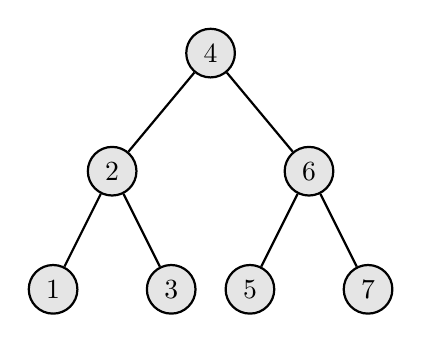
\begin{tikzpicture}
[every node/.style={draw, circle, fill=gray!20!, minimum size=5mm},
level 1/.style={sibling distance=25mm},
level 2/.style={sibling distance=15mm},
thick]
\node{4}
child{node{2} child{node{1}} child{node{3}}}
child{node{6} child{node{5}} child{node{7}}};
\end{tikzpicture}
\end{figure}

while the diagrams for the outputs are:

\begin{figure}[H]
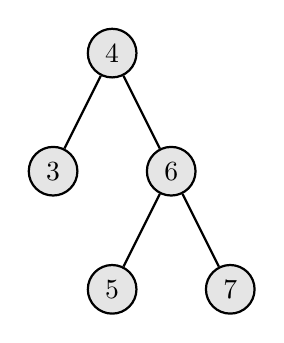
\begin{tikzpicture}
[every node/.style={draw, circle, fill=gray!20!, minimum size=5mm},
%level 1/.style={sibling distance=25mm},
%level 2/.style={sibling distance=15mm},
thick]
\node{4}
child{node{3} child[missing]}
child{node{6} child{node{5}} child{node{7}}};
\end{tikzpicture}
\end{figure}

and

\begin{figure}[H]
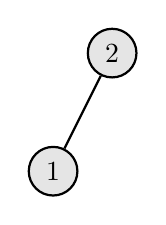
\begin{tikzpicture}
[every node/.style={draw, circle, fill=gray!20!, minimum size=5mm},
%level 1/.style={sibling distance=25mm},
%level 2/.style={sibling distance=15mm},
thick]
\node{2}
child{node{1}}
child[missing];
\end{tikzpicture}
\end{figure}

\end{flushleft}

\paragraph{Note:}

\begin{itemize}
\item The size of the BST will not exceed 50.
\item The BST is always valid and each node's value is different.
\end{itemize}

\subsection{Recursion}
For each \fcj{node} in the BST, it either belongs to the first half or the second half. Assume it belongs to the first half.

Based on the property of BST, the entire subtree at \fcj{node.left} must be in the first half. However, the subtree at \fcj{node.right} may have nodes in either halves, so it needs to be split.

We get the split result $t$ by recursively calling the function \fcj{split(node.right)}. Since \fcj{t[0]} and \fcj{t[1]} are also BST, $t[0]$ must be in the first half, and it must be to the right of \fcj{node} for the first half to be a BST. Then $t[1]$ is the second half.

\setcounter{lstlisting}{0}
\begin{lstlisting}[style=customc, caption={Recursion}]
vector<TreeNode*> splitBST( TreeNode* root, int V )
{
    if( !root )
    {
        return {nullptr, nullptr};
    }
    if( root->val <= V )
    {
        //we need to split right subtree
        auto two_trees = splitBST( root->right, V );
        //set root->right as the left part
        root->right = two_trees[0];
        //root is put in the left part
        two_trees[0] = root;
        return two_trees;
    }
    //root->val > V
    //we need to split left subtree
    auto two_trees = splitBST( root->left, V );
    //set root->left as the right part
    root->left = two_trees[1];
    //root is put in the right part
    two_trees[1] = root;
    return two_trees;
}
\end{lstlisting}
\section{777 --- Swap Adjacent in LR String}
In a string composed of \fcj{'L'}, \fcj{'R'}, and \fcj{'X'} characters, like \fcj{"RXXLRXRXL"}, a move consists of either replacing one occurrence of \fcj{"XL"} with \fcj{"LX"}, or replacing one occurrence of \fcj{"RX"} with \fcj{"XR"}. Given the starting string \fcj{start} and the ending string \fcj{end}, return \fcj{true} if and only if there exists a sequence of moves to transform one string to the other.


\paragraph{Example:}
\begin{flushleft}


\textbf{Input}: \fcj{start = "RXXLRXRXL"}, \fcj{end = "XRLXXRRLX"}

\textbf{Output}: \fcj{true}

\textbf{Explanation}:

We can transform start to end following these steps:

\fcj{RXXLRXRXL ->}

\fcj{XRXLRXRXL ->}

\fcj{XRLXRXRXL ->}

\fcj{XRLXXRRXL ->}

\fcj{XRLXXRRLX}

\end{flushleft}

\paragraph{Note:}

\begin{enumerate}
\item \fcj{1 <= len(start) = len(end) <= 10000}.

\item Both \fcj{start} and \fcj{end} will only consist of characters in \fcj{['L', 'R', 'X']}.
\end{enumerate}

\subsection{Two Scans}
One of conditions that remain true after making any move is that \fcj{'L'} and \fcj{'R'} cannot pass through each other, which means \fcj{start} and \fcj{end} strings must be the same when reading only \fcj{'L'} and \fcj{'R'}.

Another condition is 

For \fcj{'L'}, each \fcj{'L'} in \fcj{end} cannot appear in the right side of its original position in \fcj{start}. 

For \fcj{'R'}, each \fcj{'R'} in \fcj{end} cannot appear in the left side of its original position in \fcj{start}.

If above conditions can be met, we can be sure \fcj{start} can be transformed into \fcj{end}.


\setcounter{lstlisting}{0}
\begin{lstlisting}[style=customc, caption={Two Scans}]
bool canTransform( string start, string end )
{
    int count_x = 0;
    int count_L = 0;
    int count_R = 0;
    //indicate if X exists
    bool flag = false;
    for( auto i = 0ull; i < start.size(); ++i )
    {
        if( start[i] == 'X' )
        {
            ++count_x;
        }
        else if( start[i] == 'L' )
        {
            ++count_L;
        }
        else
        {
            ++count_R;
        }

        if( count_x )
        {
            flag = true;
        }
        if( end[i] == 'X' )
        {
            --count_x;
        }
        else if( end[i] == 'L' )
        {
            --count_L;
        }
        else
        {
            --count_R;
        }
    }
    if( count_x || count_L || count_R || !flag )
    {
        //no equal X, R, L
        //or no X
        return false;
    }
    auto matching_pos( 0ull );
    //compare position of L
    //L in start cannot appear left side of corresponding L in end
    for( auto i = 0ull; i < start.size(); ++i )
    {
        if( start[i] == 'L' )
        {
            //find corresponding L in end
            while( end[matching_pos] != 'L' )
            {
                ++matching_pos;
            }
            //check if corresponding L in <end> appears on right side of i
            if( i < matching_pos )
            {
                return false;
            }
            ++matching_pos;
        }
    }
    matching_pos = 0ull;
    //compare position of R
    //R in start cannot appear right side of corresponding R in end
    for( auto i = 0ull; i < start.size(); ++i )
    {
        if( start[i] == 'R' )
        {

            while( end[matching_pos] != 'R' )
            {
                ++matching_pos;
            }
            //check if corresponding R in <end> appears on left side of i
            if( i > matching_pos )
            {
                return false;
            }
            ++matching_pos;
        }
    }
    return true;
}
\end{lstlisting}

\section{778 --- Swim in Rising Water}
On an $N \times N$ grid, each square \fcj{grid[i][j]} represents the elevation at that point $(i,j)$.

Now rain starts to fall. At time $t$, the depth of the water everywhere is $t$. You can swim from a square to another 4-directionally adjacent square if and only if the elevation of both squares individually are at most t. You can swim infinite distance in zero time. Of course, you must stay within the boundaries of the grid during your swim.

You start at the top left square $(0, 0)$. What is the least time until you can reach the bottom right square $(N-1, N-1)$?

\paragraph{Example 1:}
\begin{flushleft}


\textbf{Input}: \fcj{[[0,2],[1,3]]}

\textbf{Output}: 3

\textbf{Explanation}:

At time 0, you are in grid location $ (0, 0) $.

You cannot go anywhere else because 4-directionally adjacent neighbors have a higher elevation than $ t = 0 $.

You cannot reach point $ (1, 1) $ until time 3.

When the depth of water is 3, we can swim anywhere inside the grid.
\end{flushleft}

\paragraph{Example 2:}
\begin{flushleft}
\textbf{Input}:
\fcj{[[0,1,2,3,4],[24,23,22,21,5],[12,13,14,15,16],[11,17,18,19,20],[10,9,8,7,6]]}

\textbf{Output}: 16

\textbf{Explanation}:
\[
\begin{bmatrix}
0 &  1 & 2 & 3 &  4\\
24 & 23 & 22 & 21 & 5\\
12 & 13 & 14 & 15 & 16\\
11 & 17 & 18 & 19 & 20\\
10 &  9 &  8 & 7 & 6
\end{bmatrix}
\]

The final route is marked in bold.

We need to wait until time 16 so that $ (0, 0) $ and $ (4, 4) $ are connected.

\end{flushleft}

\paragraph{Note:}

\begin{enumerate}
\item $2 \leq N \leq 50$.
\item \fcj{grid[i][j]} is a permutation of $[0, \ldots, N^2 - 1]$.
\end{enumerate}

\subsection{Heap}
We maintain a priority queue of which square we can walk in next. We always walk in the smallest one that is 4-directionally adjacent to ones we've visited.

When we reach the target, the largest number we have visited so far is the answer.

\setcounter{lstlisting}{0}
\begin{lstlisting}[style=customc, caption={Heap}]
int swimInWater( vector<vector<int>>& grid )
{
    auto N( static_cast<int>( grid.size() ) );
    //we use r * N + c to save the coord
    auto cmp = [ &grid, N ]( int p1, int p2 )
    {
        auto r1 = p1 / N;
        auto c1 = p1 - N * r1;
        auto r2 = p2 / N;
        auto c2 = p2 - N * r2;
        return grid[r1][c1] > grid[r2][c2];
    };
    //define heap
    priority_queue<int, vector<int>, decltype( cmp )> pq( cmp );
    //add (0,0)
    pq.push( 0 );
    //4 adjacent cells offset
    vector<pair<int, int>> dirs = { { -1, 0 }, { 1, 0 }, { 0, -1 }, { 0, 1 } };
    //record visited coords
    unordered_set<int> seen;
    int ans = 0;
    while( !pq.empty() )
    {
        auto t = pq.top();
        pq.pop();
        int r = t / N;
        int c = t - N * r;
        ans = ( max )( ans, grid[r][c] );
        if( ( r == N - 1 ) && ( c == N - 1 ) )
        {
            //we are at destination
            return ans;
        }
        for( int i = 0; i < 4; ++i )
        {
            auto [dr, dc] = dirs[i];
            int nr = r + dr;
            int nc = c + dc;
            if( ( nr >= 0 ) && ( nr < N ) && ( nc >= 0 ) && ( nc < N ) )
            {
                auto t = nr * N + nc;
                if( seen.find( t ) == seen.end() )
                {
                    seen.insert( t );
                    pq.push( t );
                }
            }
        }//for dirs
    }//for pq
    return -1;
}
\end{lstlisting}
\section{779 --- K-th Symbol in Grammar}
On the first row, we write a 0. Now in every subsequent row, we look at the previous row and replace each occurrence of \fcj{0} with \fcj{01}, and each occurrence of 1 with \fcj{10}.

Given row $N$ and index $K$, return the $K$--th indexed symbol in row $N$. (The values of $K$ are 1-indexed.)

\paragraph{Examples:}
\begin{flushleft}
\textbf{Input}: $N = 1$, $K = 1$

\textbf{Output}: 0

\textbf{Input}: $N = 2$, $K = 1$

\textbf{Output}: 0

\textbf{Input}: $N = 2$, $K = 2$

\textbf{Output}: 1

\textbf{Input}: $N = 4$, $K = 5$

\textbf{Output}: 1


\textbf{Explanation}:

row 1: \fcj{0}

row 2: \fcj{01}

row 3: \fcj{0110}

row 4: \fcj{01101001}

\end{flushleft}

\paragraph{Note:}

\begin{enumerate}
\item $N$ will be an integer in the range \fcj{[1, 30]}.
\item $K$ will be an integer in the range $[1, 2^{N-1}]$.
\end{enumerate}

\subsection{Recursion}
We can notice a pattern by observing a few rows: the right half is always the left half \textit{flipped}.

Therefore, if $K$ is in the right half, we could set $K\gets K - 2 ^{N-2}$ to be in the first half, and flip the final answer.

\setcounter{lstlisting}{0}
\begin{lstlisting}[style=customc, caption={Recursion}]
int kthGrammar( int N, int K )
{
    if( N == 1 )
    {
        return 0;
    }
    if( K <= ( 1 << ( N - 2 ) ) )
    {
        //K is in the left half
        //we can find in level N-1
        return kthGrammar( N - 1, K );
    }
    //K is in the right half
    //we can find in level N-1 for index K - ( 1 << ( N - 2 ) )
    //and flip the result
    return ( kthGrammar( N - 1, K - ( 1 << ( N - 2 ) ) ) ) ^ 1;
}
\end{lstlisting}

\subsection{Binary Count}
We know that right half of every row is the left half flipped.

When $K$ is written in binary (indexing from zero),  indexes of the right half of a row are ones with the first bit set to 1.

This means the number of times we flip the final answer is just the number of 1s in the binary representation of $K-1$.

\setcounter{lstlisting}{0}
\begin{lstlisting}[style=customc, caption={Bit Counts}]
int kthGrammar( int N, int K )
{
    int n = 0;
    --K;
    //the result is 1 flip
    //by the times which equal to
    //the bit 1s in K
    while( K )
    {
        K = ( K & ( K - 1 ) );
        ++n;
    }
    return n & 1;
}
\end{lstlisting}
\section{780 --- Reaching Points}
A move consists of taking a point $ (x, y) $ and transforming it to either $ (x, x+y) $ or $ (x+y, y) $.

Given a starting point  \fcj{(sx, sy)}  and a target point  \fcj{(tx, ty)} , return \fcj{true} if and only if a sequence of moves exists to transform the point \fcj{(sx, sy)} to \fcj{(tx, ty)}. Otherwise, return \fcj{false}.

\paragraph{Examples}:
\begin{flushleft}


\textbf{Input}: \fcj{sx = 1}, \fcj{sy = 1}, \fcj{tx = 3}, \fcj{ty = 5}

\textbf{Output}: \fcj{true}

\textbf{Explanation}:

One series of moves that transforms the starting point to the target is:
\fcc{(1, 1) -> (1, 2)}

\fcj{(1, 2) -> (3, 2)}

\fcj{(3, 2) -> (3, 5)}


\textbf{Input}: \fcj{sx = 1}, \fcj{sy = 1}, \fcj{tx = 2}, \fcj{ty = 2}

\textbf{Output}: \fcj{false}

\textbf{Input}: \fcj{sx = 1}, \fcj{sy = 1}, \fcj{tx = 1}, \fcj{ty = 1}

\textbf{Output}: \fcj{true}
\end{flushleft}

\paragraph{Note:}

\begin{itemize}
\item \fcj{sx}, \fcj{sy}, \fcj{tx}, \fcj{ty} will all be integers in the range $[1, 10^9]$.
\end{itemize}

\subsection{Work Backwards}
Every parent point $(x, y)$ has two children, $(x, x+y)$ and $(x+y, y)$. However, every point $(x, y)$ only has one parent candidate $(x-y, y)$ if $x \geq y$, else $(x, y-x)$.

Therefore, we can backward from \fcj{(tx, ty)} to \fcj{(sx, sy)}. For each step, we subtract the smaller one from the larger one of \fcj{tx} and \fcj{ty}. 

To speed up the process, suppose \fcj{tx > ty}. From the above analysis, we know the next operations will be \fcj{(tx-ty, ty)} until \fcj{tx = tx \% ty}. If \fcj{tx > ty} and \fcj{ty > sy}, we can combine the next operations into one operation, i.e., \fcj{tx = tx \% ty}.

Otherwise, if \fcj{ty <= sy}, we can only change \fcj{tx}. Since we can only do \fcj{tx - ty}, to reach the source point, we need \fcj{(tx - sx)} is the multiple of \fcj{ty}.

For the case \fcj{tx < ty}, the process is similar. 

When \fcj{tx = ty}, we can not make anymore movement.

\setcounter{lstlisting}{0}
\begin{lstlisting}[style=customc, caption={Bacward With Modular}]
bool reachingPoints( int sx, int sy, int tx, int ty )
{
    while( ( tx >= sx ) && ( ty >= sy ) )
    {
        if( tx == ty )
        {
            //no more move can be made
            break;
        }
        if( tx > ty )
        {
            if( ty > sy )
            {
                //we will perform tx -ty until tx < ty
                //at the end tx = tx - tx/ty*ty;
                //i.e. tx = tx mod ty;
                tx %= ty;
            }
            else
            {
                //ty <= sy
                //we can only change tx
                //so tx-n*ty=sx;
                //(tx-sx) must be multiple of ty
                return ( ( tx - sx ) % ty ) == 0;
            }
        }
        else //tx < ty
        {
            //same analysis as above
            if( tx > sx )
            {
                ty %= tx;
            }
            else
            {
                return ( ( ty - sy ) % tx ) == 0;
            }
        }
    }
    return ( tx == sx ) && ( ty == sy );
}
\end{lstlisting}
\section{781 --- Rabbits in Forest}
In a forest, each rabbit has some color. Some subset of rabbits (possibly all of them) tell you how many other rabbits have the same color as them. Those \fcj{answers} are placed in an array.

Return the minimum number of rabbits that could be in the forest.

\paragraph{Examples:}
\begin{flushleft}


\textbf{Input}: \fcj{answers = [1, 1, 2]}

\textbf{Output}: 5

\textbf{Explanation}:

The two rabbits that answered \fcj{"1"} could both be the same color, say red.

The rabbit than answered \fcj{"2"} can't be red or the answers would be inconsistent.

Say the rabbit that answered \fcj{"2"} was blue.

Then there should be 2 other blue rabbits in the forest that didn't answer into the array.

The smallest possible number of rabbits in the forest is therefore 5: 3 that answered plus 2 that didn't.

\textbf{Input}: \fcj{answers = [10, 10, 10]}

\textbf{Output}: 11

\textbf{Input}: \fcj{answers = []}

\textbf{Output}: 0
\end{flushleft}

\paragraph{Note:}

\begin{enumerate}
\item \fcj{answers} will have length at most 1000.
\item Each \fcj{answers[i]} will be an integer in the range \fcj{[0, 999]}.
\end{enumerate}

\subsection{Count}
If $ x+1 $ rabbits have same color, then we get $ x+1 $ rabbits who all answer $ x $.

now if $n$ rabbits answer $x$.

\begin{itemize}
\item If $n$ is the multiple of $x+1$, we need $n / (x + 1)$ groups of $x + 1$ rabbits.
\item Otherwise, we need $n / (x + 1) + 1$ groups of $x + 1$ rabbits.
\end{itemize}

The number of groups is \fcj{math.ceil(n / (x + 1))} which is equal to $(n+x)/(x+1)$. 

\setcounter{lstlisting}{0}
\begin{lstlisting}[style=customc, caption={Count}]
int numRabbits( vector<int>& answers )
{
    unordered_map<int, int> dict;
    for( int n : answers )
    {
        dict[n] += 1;
    }
    int ans = 0;
    for( auto[x, n] : dict )
    {
        //if n % (x+1) =0, we need n / (x+1) groups
        //otherwise, we need n / (x+1) + 1 groups
        //each group has x+1 rabbits
        //(n+x)/(x+1) covers two cases
        ans += ( x + n ) / ( x + 1 ) * ( x + 1 );
    }
    return ans;
}
\end{lstlisting}



\section{782 --- Transform to Chessboard}
An $N \times N$ \fcj{board} contains only 0s and 1s. In each move, you can swap any 2 rows with each other, or any 2 columns with each other.

What is the minimum number of moves to transform the board into a \textit{chessboard} --- a board where no 0s and no 1s are 4-directionally adjacent? If the task is impossible, return $-1$.

\paragraph{Examples:}
\begin{flushleft}
\textbf{Input}: \fcj{board = [[0,1,1,0],[0,1,1,0],[1,0,0,1],[1,0,0,1]]}

\textbf{Output}: 2

\textbf{Explanation}:

One potential sequence of moves is shown below, from left to right:

\fcj{0110     1010     1010}

\fcj{0110 --> 1010 --> 0101}

\fcj{1001     0101     1010}

\fcj{1001     0101     0101}

The first move swaps the first and second column.

The second move swaps the second and third row.

\textbf{Input}: \fcj{board = [[0, 1], [1, 0]]}

\textbf{Output}: 0

\textbf{Explanation}:

Also note that the board with 0 in the top left corner,

\fcj{01}

\fcj{10}

is also a valid chessboard.

\textbf{Input}: \fcj{board = [[1, 0], [1, 0]]}

\textbf{Output}: $-1$

\textbf{Explanation}:

No matter what sequence of moves you make, you cannot end with a valid chessboard.


\end{flushleft}
\paragraph{Note:}

\begin{itemize}
\item \fcj{board} will have the same number of rows and columns, a number in the range \fcj{[2, 30]}.
\item \fcj{board[i][j]} will be only 0s or 1s.
\end{itemize}

\subsection{Dimension}
In a valid chess board, the adjacent cells are different colors. These means, in each row and column, ones and zeros are shown in alternate order. Another property is that these rows or columns must have had half zeros and half ones, (except when the length is odd, where there could be an extra zero or one).

Furthermore, because \textbf{a row move followed by a column move is the same as a column move followed by a row move}, we can assume all the row moves happen first, then all the column moves.  (Note: it is \textit{not} true that move row $i$ then $j$ is same as moving row $j$ then $i$.)

For example, assume we have an array \fcj{[0, 1, 1, 1, 0, 0]} and the problem is to know the minimum moves to change to 0/1 alternate pattern, i.e., \fcj{[0, 1, 0, 1, 0, 1]} or \fcj{[1, 0, 1, 0, 1, 0]}.
\section{783 --- Minimum Distance Between BST Nodes}
Given a Binary Search Tree (BST) with the root node \fcj{root}, return the minimum difference between the values of any two different nodes in the tree.

\paragraph{Example:}
\begin{flushleft}


\textbf{Input}: \fcj{root = [4,2,6,1,3,null,null]}

\textbf{Output}: 1

\textbf{Explanation}:

Note that root is a TreeNode object, not an array.

The given tree \fcj{[4,2,6,1,3,null,null]} is represented by the following diagram:

\begin{figure}[H]
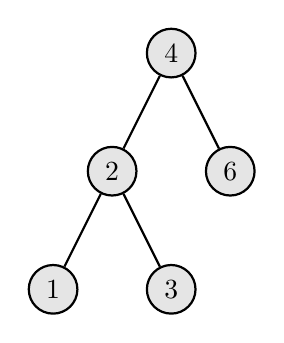
\begin{tikzpicture}
[every node/.style={draw, circle, fill=gray!20!, minimum size=5mm},
%level 1/.style={sibling distance=25mm},
%level 2/.style={sibling distance=15mm},
thick]
\node{4}
child{node{2} child{node{1}} child{node{3}}}
child{node{6}};
\end{tikzpicture}
\end{figure}


while the minimum difference in this tree is 1, it occurs between node 1 and node 2, also between node 3 and node 2.
\end{flushleft}
\paragraph{Note:}


\begin{enumerate}
\item The size of the BST will be between 2 and 100.
\item The BST is always valid, each node's value is an integer, and each node's value is different.
\end{enumerate}

\subsection{Inorder}
Inorder traversing of BST will give ascending order of values. The minimum difference only happens between two consecutive values.

\setcounter{lstlisting}{0}
\begin{lstlisting}[style=customc, caption={Inorder Traverse}]
int minDiffInBST( TreeNode* root )
{
    auto ans( INT_MAX );
    int pre = -1;
    //this flag indicate if pre is set
    bool flag = false;
    inorder( root, pre, flag, ans );
    return ans;
}
void inorder( TreeNode* node, int& pre, bool& flag, int& ans )
{
    if( !node )
    {
        return;
    }
    inorder( node->left, pre, flag, ans );
    if( !flag )
    {
        pre = node->val;
        flag = true;
    }
    else
    {
        ans = ( min )( node->val - pre, ans );
        pre = node->val;
    }
    inorder( node->right, pre, flag, ans );
}
\end{lstlisting}
\section{784 --- Letter Case Permutation}
Given a string $S$, we can transform every letter individually to be lowercase or uppercase to create another string.  Return a list of all possible strings we could create.

\paragraph{Examples:}
\begin{flushleft}


\textbf{Input}: \fcj{S = "a1b2"}

\textbf{Output}: \fcj{["a1b2", "a1B2", "A1b2", "A1B2"]}

\textbf{Input}: \fcj{S = "3z4"}

\textbf{Output}: \fcj{["3z4", "3Z4"]}

\textbf{Input}: \fcj{S = "12345"}

\textbf{Output}: \fcj{["12345"]}

\end{flushleft}

\paragraph{Note:}

\begin{enumerate}
\item $S$ will be a string with length between 1 and 12.
\item $S$ will consist only of letters or digits.
\end{enumerate}
\section{785 --- Is Graph Bipartite?}
Given an undirected \fcj{graph}, return \fcj{true} if and only if it is bipartite.

Recall that a graph is \textbf{bipartite} if we can split it's set of nodes into two independent subsets A and B such that every edge in the graph has one node in A and another node in B.

The graph is given in the following form: \fcj{ graph[i]} is a list of indexes $j$ for which the edge between nodes $i$ and $j$ exists. Each node is an integer between 0 and \fcj{graph.length - 1}.  There are no self edges or parallel edges: \fcj{graph[i]} does not contain $i$, and it doesn't contain any element twice.

\paragraph{Example 1:}
\begin{flushleft}
\textbf{Input}: \fcj{[[1,3], [0,2], [1,3], [0,2]]}

\textbf{Output}: true

\textbf{Explanation}: 

The graph looks like this:
\begin{figure}[H]
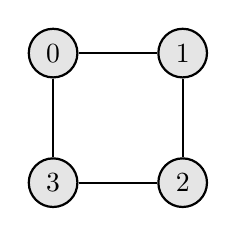
\begin{tikzpicture}
[every node/.style={draw, circle, fill=gray!20!, minimum size=5mm},
thick]
\node(0){0};
\node(1)[right=1cm of 0]{1};
\node(2)[below=1cm of 1]{2};
\node(3)[below=1cm of 0]{3};
\draw (0) -- (1) -- (2) -- (3) -- (0);
\end{tikzpicture}
\end{figure}
%0----1
%|    |
%|    |
%3----2
We can divide the vertices into two groups: \fcj{(0, 2)} and \fcj{(1, 3)}.


\end{flushleft}

\paragraph{Example 2:}

\begin{flushleft}
\textbf{Input}: \fcj{[[1,2,3], [0,2], [0,1,3], [0,2]]}

\textbf{Output}: \fcj{false}

\textbf{Explanation}: 

The graph looks like this:

\begin{figure}[H]
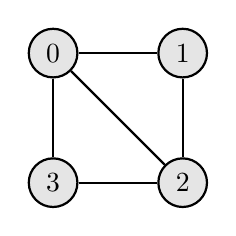
\begin{tikzpicture}
[every node/.style={draw, circle, fill=gray!20!, minimum size=5mm},
thick]
\node(0){0};
\node(1)[right=1cm of 0]{1};
\node(2)[below=1cm of 1]{2};
\node(3)[below=1cm of 0]{3};
\draw (0) -- (1) -- (2) -- (3) -- (0);
\draw (0) -- (2);
\end{tikzpicture}
\end{figure}

%0----1
%| \  |
%|  \ |
%3----2
We cannot find a way to divide the set of nodes into two independent subsets.


\end{flushleft}

\paragraph{Note:}

\begin{itemize}
\item \fcj{graph} will have length in range \fcj{[1, 100]}.
\item \fcj{graph[i]} will contain integers in range \fcj{[0, graph.length - 1]}.
\item \fcj{graph[i]} will not contain $i$ or duplicate values.
\item The graph is undirected: if any element $j$ is in \fcj{graph[i]}, then $i$ will be in \fcj{graph[j]}.
\end{itemize}

\subsection{Coloring Node}
For each uncolored node, we start the coloring process by doing a \textbf{DFS} on that node. Every neighbor gets colored the opposite color from the current node. If we find a neighbor colored the same color as the current node, then our coloring was impossible.


\setcounter{lstlisting}{0}
\begin{lstlisting}[style=customc, caption={DFS}]
bool isBipartite( vector<vector<int>>& graph )
{
    auto N( static_cast< int >( graph.size() ) );
    vector<int> colors( N, -1 );
    for( int i = 0; i < N; ++i )
    {
        if( colors[i] == -1 )
        {
            //node i is not colored
            //color i with color 1
            colors[i] = 1;
            //start dfs
            stack<int> stk;
            stk.push( i );
            while( !stk.empty() )
            {
                int node = stk.top();
                stk.pop();
                //visit adjacent nodes
                for( int adj : graph[node] )
                {
                    if( colors[adj] == -1 )
                    {
                        //this adjacent node is not colored
                        stk.push( adj );
                        //color it as inverse color of node
                        colors[adj] = 1 - colors[node];
                    }
                    else if( colors[adj] == colors[node] )
                    {
                        //the adjacent node has same color with node
                        //we cannot bipartite the graph
                        return false;
                    }
                }//for(adj)
            }//while(stk)
        }//if(color)
    }//for(i)
    return true;
}
\end{lstlisting}
\section{786 --- K-th Smallest Prime Fraction}
A sorted list $A$ contains 1, plus some number of primes. Then, for every $p < q$ in the list, we consider the fraction $p/q$.

What is the $K$-th smallest fraction considered?  Return your answer as an array of ints, where \fcj{answer[0] = p} and \fcj{answer[1] = q}.

\paragraph{Examples:}
\begin{flushleft}


\textbf{Input}: \fcj{A = [1, 2, 3, 5]}, $K = 3$

\textbf{Output}: \fcj{[2, 5]}

\textbf{Explanation}:

The fractions to be considered in sorted order are:

$1/5$, $1/3$, $2/5$, $1/2$, $3/5$, $2/3$.

The third fraction is 2/5.

\textbf{Input}: \fcj{A = [1, 7]}, \fcj{K = 1}

\textbf{Output}: \fcj{[1, 7]}

\end{flushleft}

\paragraph{Note:}

\begin{enumerate}
\item $A$ will have length between 2 and 2000.

\item Each \fcj{A[i]} will be between 1 and 30000.

\item $K$ will be between 1 and \fcj{A.length * (A.length - 1) / 2}.
\end{enumerate}

\subsection{Binary Search}
The fraction range will be $(0, 1)$. Suppose $f(x)$ be the number of fractions below $x$. It's an increasing function on $x$, so we can binary search for the correct answer.

During the finding of $x$ such that there are exactly $K$ fractions below $x$, we record the largest fraction which is less than $x$.

\setcounter{lstlisting}{0}
\begin{lstlisting}[style=customc, caption={Binary Search}]
vector<int> kthSmallestPrimeFraction( vector<int>& A, int K )
{
    auto hi( 1.0 );
    auto lo( 0.0 );
    auto norm( 0 );
    auto denorm( 1 );
    auto count( 0 );
    vector<int> ans( 2 );
    while( hi - lo > 1e-9 )
    {
        auto mid( hi * .5 + lo * .5 );
        //get the count of fractions less than x
        get_count( A, mid, norm, denorm, count );

        if( count < K )
        {
            //search in higher half
            lo = mid;
        }
        else
        {
            //search in lower half
            hi = mid;
            //record norm/denorm
            ans[0] = norm;
            ans[1] = denorm;
        }
    }
    return ans;
}
//helper function to get
//number of fractions less than x
void get_count( vector<int>& A, double x, int& norm, int& denorm, int& count )
{
    norm = 0;
    denorm = 1;
    count = 0;
    auto L( static_cast< int >( A.size() ) );
    int left = -1;
    for( int right = 1; right < L; ++right )
    {
        while( static_cast< double >( A[left + 1] ) / static_cast< double >( A[right] ) < x )
        {
            ++left;
        }
        //when left = -1
        //left +1=0, this is a very good trick
        count += ( left + 1 );
        //get maximum fraction so far
        if( ( left >= 0 ) && ( norm * A[right] < denorm * A[left] ) )
        {
            norm = A[left];
            denorm = A[right];
        }
    }
}
\end{lstlisting}
\section{787 --- Cheapest Flights Within K Stops}
There are $n$ cities connected by $m$ flights. Each fight starts from city $u$ and arrives at $v$ with a price $w$.

Now given all the cities and flights, together with starting city \fcj{src} and the destination \fcj{dst}, your task is to find the cheapest price from \fcj{src} to \fcj{dst} with up to $k$ stops. If there is no such route, output $-1$.

\paragraph{Example 1:}

\begin{flushleft}
\textbf{Input}: 

$n = 3$, \fcj{edges = [[0,1,100],[1,2,100],[0,2,500]]}

\fcj{src = 0}, \fcj{dst = 2}, $k = 1$

\textbf{Output}: 200

\textbf{Explanation}: 

The graph looks like this:

\begin{figure}[H]
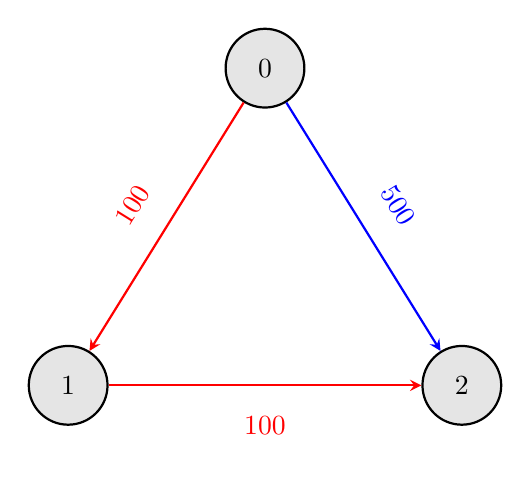
\begin{tikzpicture}
[every node/.style={draw, circle, fill=gray!20!, minimum size=1cm},
thick, >=stealth, ->]
\node(0){0};
\node(1)[below=3cm of 0, xshift=-2.5cm]{1};
\node(2)[below=3cm of 0, xshift=2.5cm]{2};
\draw[red] (0) -- (1) node[sloped, above, draw=none, fill=none, pos=0.5, auto]{100};
\draw[red] (1) -- (2) node[sloped, below, draw=none, fill=none, pos=0.5]{100};
\draw[blue] (0) -- (2) node[sloped, above, draw= none, fill=none, pos=0.5]{500};
\end{tikzpicture}
\end{figure}

The cheapest price from city 0 to city 2 with at most 1 stop costs 200, as marked red in the picture.

\end{flushleft}

\paragraph{Example 2:}

\begin{flushleft}


\textbf{Input}: 

$ n = 3 $, \fcj{edges = [[0,1,100],[1,2,100],[0,2,500]]}

\fcj{src = 0}, \fcj{dst = 2}, $k = 0$

\textbf{Output}: 500

\textbf{Explanation}: 

The graph looks like this:

\begin{figure}[H]
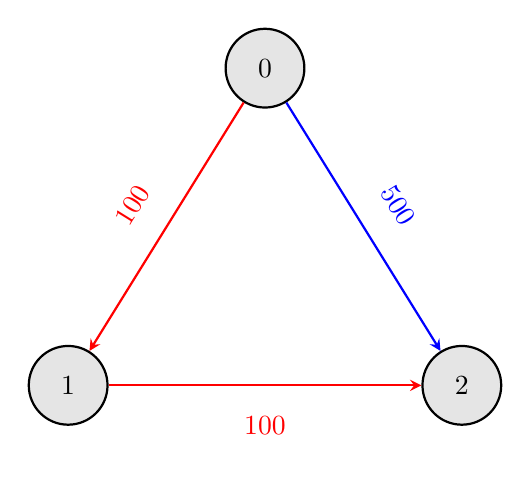
\begin{tikzpicture}
[every node/.style={draw, circle, fill=gray!20!, minimum size=1cm},
thick, >=stealth, ->]
\node(0){0};
\node(1)[below=3cm of 0, xshift=-2.5cm]{1};
\node(2)[below=3cm of 0, xshift=2.5cm]{2};
\draw[red] (0) -- (1) node[sloped, above, draw=none, fill=none, pos=0.5, auto]{100};
\draw[red] (1) -- (2) node[sloped, below, draw=none, fill=none, pos=0.5]{100};
\draw[blue] (0) -- (2) node[sloped, above, draw= none, fill=none, pos=0.5]{500};
\end{tikzpicture}
\end{figure}

The cheapest price from city 0 to city 2 with at most 0 stop costs 500, as marked blue in the picture.

\end{flushleft}


\paragraph{Note:}

\begin{itemize}
\item The number of nodes $n$ will be in range \fcj{[1, 100]}, with nodes labeled from 0 to $n - 1$.
\item The size of flights will be in range $[0, n \times (n - 1) / 2]$.
\item The format of each flight will be \fcj{(src, dst, price)}.
\item The price of each flight will be in the range \fcj{[1, 10000]}.
\item $k$ is in the range of $[0, n - 1]$.
\item There will not be any duplicated flights or self cycles.
\end{itemize}

\subsection{Bellman Ford}
This algorithm is based on \textbf{DP}. We utilize a 2-d function $F$ where $F(i,j)$ means the minimum price to destination $i$ by taking at most $j$ stops. 

We iterate stops from 1 to $K+1$ (we need one more stop to get to destination), to fill $F$. For \fcj{src}, we always set its value to zero no matter how many stops.

\setcounter{lstlisting}{0}
\begin{lstlisting}[style=customc, caption={2D DP}]
int findCheapestPrice( int n, vector<vector<int>>& flights, int src, int dst, int K )
{
    auto max_prc( 100000 );
    vector<vector<int>> F( n, vector<int>( K + 2, max_prc ) );
    F[src][0] = 0;
    for( int stops = 1; stops <= K + 1; ++stops )
    {
        //cost for src with any stops
        //is zero
        F[src][stops] = 0;
        //Fill F
        for( const auto& flight : flights )
        {
            int from = flight[0];
            int to = flight[1];
            int prc = flight[2];
            //F[from][stops-1]: the cost to fly to <from> with stops-1
            F[to][stops] = ( min )( F[from][stops - 1] + prc, F[to][stops] );
        }
    }
    return F[dst][K + 1] == max_prc ? -1 : F[dst][K + 1];
}
\end{lstlisting}

We can reduce memory usage by changing the 2D to 1D \textbf{DP} with two 1D arrays. One array is used to get next iteration result.

\begin{lstlisting}[style=customc, caption={1D DP}]
int findCheapestPrice( int n, vector<vector<int>>& flights, int src, int dst, int K )
{
    auto max_prc( 100000 );
    vector<int> F( n, max_prc );
    F[src] = 0;
    for( int stops = 1; stops <= K + 1; ++stops )
    {
        F[src] = 0;

        //used to current iteration result
        vector<int> NF( F );
        for( const auto& flight : flights )
        {
            int from = flight[0];
            int to = flight[1];
            int prc = flight[2];
            NF[to] = ( min )( F[from] + prc, NF[to] );
        }
        swap( NF, F );
    }
    return F[dst] == max_prc ? -1 : F[dst];
}
\end{lstlisting}



\section{788 --- Rotated Digits}
$X$ is a good number if after rotating each digit individually by 180 degrees, we get a valid number that is different from $X$.  Each digit must be rotated - we cannot choose to leave it alone.

A number is valid if each digit remains a digit after rotation. 0, 1, and 8 rotate to themselves; 2 and 5 rotate to each other; 6 and 9 rotate to each other, and the rest of the numbers do not rotate to any other number and become invalid.

Now given a positive number $N$, how many numbers $X$ from $1$ to $N$ are good?

\paragraph{Example:}

\begin{flushleft}
\textbf{Input}: 10

\textbf{Output}: 4

\textbf{Explanation}: 

There are four good numbers in the range \fcj{[1, 10]} : 2, 5, 6, 9.

Note that 1 and 10 are not good numbers, since they remain unchanged after rotating.
\end{flushleft}

\paragraph{Note:}

\begin{itemize}
\item $N$  will be in range \fcj{[1, 10000]}.
\end{itemize}

\subsection{Dynamic Programming}
Let $F$ is the DP array with size $N+1$. Each element in $F$ has three states:

\begin{itemize}
\item 0 --- invalid after rotation.
\item 1 --- same as before after rotation
\item 2 --- different number after rotation.
\end{itemize}

For numbers less than 10, we will have 

\begin{itemize}
\item $F[3]=F[4]=F[7]=0$
\item $F[0]=F[1]=F[8]=1$
\item $F[2]=F[5]=F[6]=F[9]=2$
\end{itemize}

Then for each number $x\geq 10$, $F[x]$ can be built from $F[x/10]$ and $F[\bmod(x,10)]$.

When $F[x/10]=1$ and $F[\bmod(x, 10)]=1$, we know that $F[x]=1$ (same as before).

When  one of them is 2, and another one is equal or larger than 1, we know $F[x]=2$ (valid after rotation). 

In other cases, $F[x]=0$.

\setcounter{lstlisting}{0}
\begin{lstlisting}[style=customc, caption={DP}]
int rotatedDigits( int N )
{
    vector<unsigned char> F( N + 1, 0 );
    int ans = 0;
    for( int i = 0; i <= ( min )( 9, N ); ++i )
    {
        if( ( i == 1 ) || ( i == 0 ) || ( i == 8 ) )
        {
            F[i] = 1;
        }
        else if( ( i == 2 ) || ( i == 5 ) || ( i == 6 ) || ( i == 9 ) )
        {
            F[i] = 2;
            ++ans;
        }
    }
    if( N < 10 )
    {
        return ans;
    }
    for( int i = 10; i <= N; ++i )
    {
        int q = i / 10;
        int r = i - q * 10;

        if( ( F[q] == 1 ) && ( F[r] == 1 ) )
        {
            //remain the same
            F[i] = 1;
        }
        else if( ( F[q] >= 1 ) && ( F[r] >= 1 ) )
        {
            //valid after rotate
            F[i] = 2;
            ++ans;
        }
    }
    return ans;
}
\end{lstlisting}
\section{789 --- Escape The Ghosts}
You are playing a simplified Pacman game. 

You start at the point \fcj{(0, 0)}, and your destination is \fcj{(target[0], target[1])}. There are several ghosts on the map, the $i$--th ghost starts at \fcj{(ghosts[i][0], ghosts[i][1])}.

Each turn, you and all ghosts simultaneously *may* move in one of 4 cardinal directions: north, east, west, or south, going from the previous point to a new point 1 unit of distance away.

You escape if and only if you can reach the target before any ghost reaches you (for any given moves the ghosts may take.)  If you reach any square (including the target) at the same time as a ghost, it doesn't count as an escape.

Return \fcj{true} if and only if it is possible to escape.

\paragraph{Example 1:}

\begin{flushleft}
\textbf{Input}: 

\fcj{ghosts = [[1, 0], [0, 3]]}

\fcj{target = [0, 1]}

\textbf{Output}: \fcj{true}

\textbf{Explanation}: 

You can directly reach the destination \fcj{(0, 1)} at time 1, while the ghosts located at \fcj{(1, 0)} or \fcj{(0, 3)} have no way to catch up with you.

\end{flushleft}

\paragraph{Example 2:}

\begin{flushleft}

\textbf{Input}: 

\fcj{ghosts = [[1, 0]]}

\fcj{target = [2, 0]}

\textbf{Output}: \fcj{false}

\textbf{Explanation}: 

You need to reach the destination (2, 0), but the ghost at (1, 0) lies between you and the destination.

\end{flushleft}

\paragraph{Example 3:}

\begin{flushleft}
\textbf{Input}: 

\fcj{ghosts = [[2, 0]]}

\fcj{target = [1, 0]}

\textbf{Output}: \fcj{false}

\textbf{Explanation}: 

The ghost can reach the target at the same time as you.

\end{flushleft}

\paragraph{Note:}

\begin{itemize}
\item All points have coordinates with absolute value \fcj{<= 10000}.
\item The number of ghosts will not exceed 100.
\end{itemize}

\subsection{Taxicab Distance}
The taxicab distance is the number of moves required to get from point A to point B in our grid. It is calculated as 

\fcj{dist(A, B) = abs(A.x - B.x) + abs(A.y - B.y)}.

Let's say we start at $S$, the ghost starts at $G$, the target is $T$, and the ghost first meets us at $X$. This implies 

\fcj{dist(G, X) <= dist(S, X)}, 

as the ghost must reach X before or at the time that we do.

Now, if the ghost travels from $G$ to $X$ and then to $T$, it will reach T at time 

\fcj{dist(G, T) <= dist(G, X) + dist(X, T) <= dist(S, X) + dist(X, T)}.

The first inequality is because of the triangle inequality that all distance metrics satisfy.

The above shows that it is at least as good for the ghost to just travel directly to the target: if it could reach us beforehand (at $X$), it will also reach us if it goes to $X$ then to $T$, and then it would reach us if it just went directly to $T$.

Also, if the ghost goes directly to the target, then a necessary condition is clearly that we get to the target before the ghost.

Once we can make the assumption that all parties just go directly to the target in the shortest time possible, the problem is greatly simplified.

\setcounter{lstlisting}{0}
\begin{lstlisting}[style=customc, caption={Taxicab Distance}]
bool escapeGhosts( vector<vector<int>>& ghosts, vector<int>& target )
{
    auto taxicab_dist = [&target]( const vector<int>& P )
    {

        return abs( P[0] - target[0] ) + abs( P[1] - target[1] );
    };
    //the taxicab distance from source to target
    int dist = abs( target[0] ) + abs( target[1] );
    for( const auto& ghost : ghosts )
    {
        if( taxicab_dist( ghost ) <= dist )
        {
            //this ghost cannot be avoid
            return false;
        }
    }
    return true;
}
\end{lstlisting}
%\include{790}
\section{791 --- Custom Sort String}
$S$ and $T$ are strings composed of lowercase letters. In $S$, no letter occurs more than once.

$S$ was sorted in some custom order previously. We want to permute the characters of $T$ so that they match the order that $S$ was sorted. More specifically, if $x$ occurs before $y$ in $S$, then $x$ should occur before $y$ in the returned string.

Return any permutation of $T$ (as a string) that satisfies this property.

\paragraph{Example:}
\begin{flushleft}


\textbf{Input}: 

\fcj{S = "cba"}

\fcj{T = "abcd"}

\textbf{Output}: \fcj{"cbad"}

\textbf{Explanation}: 

\fcj{"a"}, \fcj{"b"}, \fcj{"c"} appear in $S$, so the order of \fcj{"a"}, \fcj{"b"}, \fcj{"c"} should be \fcj{"c"}, \fcj{"b"}, and \fcj{"a"}.
 
Since \fcj{"d"} does not appear in $S$, it can be at any position in $T$. \fcj{"dcba"}, \fcj{"cdba"}, \fcj{"cbda"} are also valid outputs.
 
\end{flushleft}

\paragraph{Note:}

\begin{itemize}
\item $S$ has length at most 26, and no character is repeated in $S$.
\item $T$ has length at most 200.
\item $S$ and $T$ consist of lowercase letters only.
\end{itemize}

\subsection{Count And Write}
First, count elements in $T$ and then traversing $S$. write those elements in the order in $S$. Then add those letters do not appear in $S$.

\setcounter{lstlisting}{0}
\begin{lstlisting}[style=customc, caption={Count And Write}]
string customSortString( string S, string T )
{
    vector<int> dict( 26, 0 );

    //count letters in T
    for( auto c : T )
    {
        dict[c - 'a'] += 1;
    }
    string ans;
    ans.reserve( T.size() );
    for( auto c : S )
    {
        if( dict[c - 'a'] > 0 )
        {
            //we add this letter first
            ans.append( dict[c - 'a'], c );
            dict[c - 'a'] = 0;
        }
    }
    //then add letters do not appear in S
    for( int i = 0; i < 26; ++i )
    {
        if( dict[i] > 0 )
        {
            ans.append( dict[i], 'a' + i );
        }
    }
    return ans;
}
\end{lstlisting}
\section{792 --- Number of Matching Subsequences}
Given string $S$ and a dictionary of words \fcj{words}, find the number of \fcj{words[i]} that is a subsequence of $S$.

\paragraph{Example:}

\begin{flushleft}
\textbf{Input}: 

\fcj{S = "abcde"}

\fcj{words = ["a", "bb", "acd", "ace"]}

\textbf{Output}: 3

\textbf{Explanation}: There are three words in words that are a subsequence of S: \fcj{"a"}, \fcj{"acd"}, \fcj{"ace"}.
\end{flushleft}

\paragraph{Note:}

\begin{itemize}
\item All words in \fcj{words} and $S$ will only consists of lowercase letters.
\item The length of $S$ will be in the range of \fcj{[1, 50000]}.
\item The length of \fcj{words} will be in the range of \fcj{[1, 5000]}.
\item The length of \fcj{words[i]} will be in the range of \fcj{[1, 50]}.
\end{itemize}

\subsection{Next Letter Position}
Since the length of $S$ is large, we need to only iterate over it for once.

We can put words into buckets by starting character. Take the given example, we put each word in \fcj{words} into two buckets which are

\fcj{'a': (0,1), (2,1), {3,1}}

\fcj{'b': (1,1)}

Each bucket has pairs associated with each letter. The first number is the index of this word in \fcj{words} and the 2nd one is the position of next letter in this word.

Then we iterate over $S$. The first letter is \fcj{'a'}. Thus, we process the bucket for letter \fcj{'a'}, the three pairs are processed as below

\begin{enumerate}
\item \fcj{(0,1)}: next letter's position is 1 and word \fcj{"a"} length is 1. Thus, this is the subsequence of $S$.
\item \fcj{(2,1)}: The word is \fcj{"acd"} and the next letter is \fcj{'c'}. We create a new bucket which is \fcj{'c'} and the first associated pair will be \fcj{(2,2)} because \fcj{"acd"} has index 2 and next letter of \fcj{'c'} has index 2 in \fcj{"acd"}.
\item \fcj{(3,1)}: The word is \fcj{"ace"}, and the next letter is \fcj{'c'}. We have already created bucket for \fcj{'c'}. This time we add a new pair \fcj{3,2} because \fcj{"ace"} has index 3 and next letter of \fcj{'c'} has index 2 in \fcj{"acd"}.
\end{enumerate}

Thus, after processing bucket of \fcj{'a'}, we have 

\fcj{'b': (1,1)}

\fcj{'c': (2,2), (3,2)}

The next letter in $S$ is \fcj{'b'}. Similarly, after processing for bucket of \fcj{'b'}, we have

\fcj{'b': (1,2)}

\fcj{'c': (2,2), (3,2)}

Then process bucket of \fcj{'c'}, the processing results will be 

\fcj{'b': (1,2)}

\fcj{'d': (3,3)}

\fcj{'e': (2,3)}

Next letter in $S$ is \fcj{'d'}. When processing bucket of \fcj{'d'}, we found that the next letter's position is 3 which is the length of \fcj{"acd"}. Thus, this word is a subsequence of $S$. Now, we have two buckets

\fcj{'b': (1,2)}

\fcj{'e': (2,3)}

The last letter is \fcj{'e'} and also this reach the end of \fcj{'ace'}. Finally, we have only one bucket left

\fcj{'b': (1,2)}

Thus the word at index 1 of \fcj{words}, i.e., \fcj{"bb"} is not subsequence of $S$.

\setcounter{lstlisting}{0}
\begin{lstlisting}[style=customc, caption={Next Letter Position}]
int numMatchingSubseq( string S, vector<string>& words )
{
    vector<vector<pair<size_t, size_t>>> buckets( 26 );
    auto wi( 0ull );
    for( const auto& word : words )
    {
        //create bucket for first letter
        //which contains a few pairs (word_index, next letter index)
        //Since this is the first letter in word
        //next letter index is 1
        buckets[word[0] - 'a'].emplace_back( wi, 1 );
        ++wi;
    }
    auto ans( 0 );
    for( auto c : S )
    {
        decltype( buckets )::value_type vec_pairs;
        swap( vec_pairs, buckets[c - 'a'] );
        for( auto [wi, ci] : vec_pairs )
        {
            if( ci == words[wi].size() )
            {
                //we reach the end of words[wi]
                //this is the subsequence of S
                ++ans;
            }
            else
            {
                const auto& word( words[wi] );
                //create another bucket
                //with pair (wi, ci+1).
                //ci+1 is next letter index
                buckets[word[ci] - 'a'].emplace_back( wi, ci + 1 );
            }
        }
    }
    return ans;
}
\end{lstlisting}
\section{793 --- Preimage Size of Factorial Zeroes Function}

\textbf{Hard}

Let $ f(x) $ be the number of zeroes at the end of $ x! $. (Recall that $ x! = 1 \times 2 \times 3 \times \ldots \times x $, and by convention, $0! = 1$.)

For example, $ f(3) = 0 $ because $ 3! = 6 $ has no zeroes at the end, while $ f(11) = 2 $ because $ 11! = 39916800 $ has 2 zeroes at the end. Given $ K $, find how many non-negative integers $ x $ have the property that $ f(x) = K $.

\paragraph{Example 1:}

\begin{flushleft}
\textbf{Input}: K = 0

\textbf{Output}: 5

\textbf{Explanation}: 0!, 1!, 2!, 3!, and 4! end with K = 0 zeroes.
\end{flushleft}

\paragraph{Example 2:}

\begin{flushleft}
\textbf{Input}: $ K = 5 $

\textbf{Output}: 0

\textbf{Explanation}: There is no $ x $ such that $ x! $ ends in $ K = 5 $ zeroes.
\end{flushleft}

\paragraph{Note:}

\begin{itemize}
\item $ K $ will be an integer in the range $ [0, 10^9] $.
\end{itemize}

\subsection{Binary Search}

Denote $\zeta(x)$ be the number of zeroes at the end of $x!$. If the prime factorization of $ x! $ is $ (2^a * 5^b * \cdots )$, the number of times that 10 divides this is $\min(a, b)$ which is $b$ (number of 5 multiples are less than number of 2 multiples).

Thus, $\zeta(x)$ is the number of times 5 divides $ x! $, which is equal to 

$ \lfloor \frac{x}{5^1} \rfloor + \lfloor \frac{x}{5^2} \rfloor + \lfloor \frac{x}{5^3} \rfloor + \lfloor \frac{x}{5^4} \rfloor + \cdots $

Indeed, $\zeta$ is a monotone increasing function, so we can for both the \textbf{largest} and \textbf{smallest} value $ x $ such that $ \zeta(x) = K $. However, since $ \zeta(5a-1) < \zeta(5a) = \zeta(5a+1) = \zeta(5a+2) = \zeta(5a+3) = \zeta(5a+4) < \zeta(5a+5) $, if it is possible for $ \zeta(x) $ to equal $ K $ for some $ x $, return 5, else the answer is 0.

\setcounter{lstlisting}{0}
\begin{lstlisting}[style=customc, caption={Binary Search}]
int preimageSizeFZF( int K )
{
    //notice: we need long long data type
    //to avoid overflow
    long long lo( K );
    long long hi( lo * 10 + 1 );
    //standard binary search
    while( lo <= hi )
    {
        auto mid( lo + ( hi - lo ) / 2 );
        auto zeros( trail_zeros( mid ) );
        if( zeros == K )
        {
            //only five number can have K
            //zeros
            return 5;
        }
        if( zeros < K )
        {
            lo = mid + 1;
        }
        else
        {
            hi = mid - 1;
        }
    }
    return 0;
}
//helper function to get number of trailing zeros
//same as problem 173
int trail_zeros( long long n )
{
    int zeros = 0;
    while( n )
    {
        zeros += n / 5;
        n = n / 5;
    }
    return zeros;
}
\end{lstlisting}
\section{794 --- Valid Tic-Tac-Toe State}

\textbf{Medium}

A Tic-Tac-Toe board is given as a string array \fcj{board}. Return \fcj{true} if and only if it is possible to reach this board position during the course of a valid tic-tac-toe game.

The board is a $ 3 \times 3 $ array, and consists of characters \fcj{" "}, \fcj{"X"}, and \fcj{"O"}.  The \fcj{" "} character represents an empty square.

Here are the rules of Tic-Tac-Toe:

\begin{itemize}
\item Players take turns placing characters into empty squares (\fcj{" "}).

\item The first player always places \fcj{"X"} characters, while the second player always places \fcj{"O"} characters.

\item \fcj{"X"} and \fcj{"O"} characters are always placed into empty squares, never filled ones.

\item The game ends when there are 3 of the same (non-empty) character filling any row, column, or diagonal.

\item The game also ends if all squares are non-empty.

\item No more moves can be played if the game is over.
\end{itemize}

\paragraph{Example 1:}

\begin{flushleft}
\textbf{Input}: \fcj{board = ["O  ", "   ", "   "]}

\textbf{Output}: \fcj{false}

\textbf{Explanation}: The first player always plays \fcj{"X"}.
\end{flushleft}

\paragraph{Example 2:}

\begin{flushleft}
\textbf{Input}: \fcj{board = ["XOX", " X ", "   "]}

\textbf{Output}: \fcj{false}

\textbf{Explanation}: Players take turns making moves.
\end{flushleft}

\paragraph{Example 3:}

\begin{flushleft}
\textbf{Input}: \fcj{board = ["XXX", "   ", "OOO"]}

\textbf{Output}: \fcj{false}
\end{flushleft}

\paragraph{Example 4:}

\begin{flushleft}
\textbf{Input}: \fcj{board = ["XOX", "O O", "XOX"]}

\textbf{Output}: \fcj{true}
\end{flushleft}

\paragraph{Note:}

\begin{itemize}
\item board is a length-3 array of strings, where each string \fcj{board[i]} has length 3.
\item Each \fcj{board[i][j]} is a character in the set \fcj{[" ", "X", "O"]}.
\end{itemize}

\subsection{Ad Hoc}
Since players take turns, the number of \fcj{'X'} must be equal to or one greater than the number of \fcj{'O'}.

\begin{enumerate}
\item If the first player wins, the number of \fcj{'X'} is one more than the number of \fcj{'O'}.

\item If the second player wins, the number of \fcj{'X'}s is equal to the number of \fcj{'O'}.

\item The board can't simultaneously have three \fcj{'X'} and three \fcj{'O'} in a row, and once one player has won (on their move), there are no subsequent moves.
\end{enumerate}


It turns out these conditions are also sufficient to check the validity of all boards. 

For the first two cases, count the number of \fcj{'X'} and \fcj{'O'}.

As to the 3rd case, use a helper function \fcj{win(player)} to check if that \fcj{player} has won. This checks the 8 horizontal, vertical, or diagonal lines of the board to find if there are three in a row equal to that player.


\setcounter{lstlisting}{0}
\begin{lstlisting}[style=customc, caption={Ad Hoc}]
bool validTicTacToe( vector<string>& board )
{
    auto count_X( 0 );
    auto count_O( 0 );
    for( const auto& row : board )
    {
        for( auto c : row )
        {
            if( c == 'X' )
            {
                count_X += 1;
            }
            else if( c == 'O' )
            {
                count_O += 1;
            }
        }
    }
    //num(x)==num(o) or num(x)==num(o) + 1
    if( ( count_X != count_O ) && ( count_X != count_O + 1 ) )
    {
        return false;
    }
    //if X wins, num(x)=num(o)+1 because X play first
    if( can_win( board, 'X' ) && ( count_X != count_O + 1 ) )
    {
        return false;
    }
    //if O wins, num(x)=num(o) because X play first
    if( can_win( board, 'O' ) && ( count_X != count_O ) )
    {
        return false;
    }
    return true;
}
//check if player wins
//any row, column, diagnaol or anti-diagnaol
//have same kind of player
bool can_win( const vector<string>& b, char player )
{
    for( int i = 0; i < 3; ++i )
    {
        //horizon
        if( ( b[i][0] == player ) && ( b[i][1] == player ) && ( b[i][2] == player ) )
        {
            return true;
        }

        //vertical
        if( ( b[0][i] == player ) && ( b[1][i] == player ) && ( b[2][i] == player ) )
        {
            return true;
        }
    }

    //diagnaol
    if( ( b[0][0] == player ) && ( b[1][1] == player ) && ( b[2][2] == player ) )
    {
        return true;
    }
    //aniti-diagnaol
    if( ( b[2][0] == player ) && ( b[1][1] == player ) && ( b[0][2] == player ) )
    {
        return true;
    }
    return false;
}
\end{lstlisting}
\section{795 --- Number of Subarrays with Bounded Maximum}

\textbf{Medium}

We are given an array $A$ of positive integers, and two positive integers $L$ and $R$ ($L \leq R$).

Return the number of (contiguous, non-empty) subarrays such that the value of the maximum array element in that subarray is at least $L$ and at most $R$.

\paragraph{Example :}
\begin{flushleft}


\textbf{Input}: 

\fcj{A = [2, 1, 4, 3]}

$ L = 2 $

$ R = 3 $

\textbf{Output}: 3

\textbf{Explanation}: 

There are three subarrays that meet the requirements: \fcj{[2]}, \fcj{[2, 1]}, \fcj{[3]}.
\end{flushleft}

\paragraph{Note:}

\begin{enumerate}
\item $L$, $R$  and \fcj{A[i]} will be an integer in the range $[0, 10^9]$.
\item The length of $A$ will be in the range of \fcj{[1, 50000]}.
\end{enumerate}

\subsection{Counting}
As we only care about whether each element is less than, between, or greater than the interval $ [L, R] $, we can mark each element is either $a$ if it is less than $L$; $b$ if it is between $L$ and $R$; or $c$ if it is greater than $R$.

Then, we want the number of subarrays with no $c$ and at least one $b$. $c$ split the array into groups of arrays with only $a$ and $b$. For example, if the given array is \fcj{[a, a, b, c, c, b, a, c, a]}, then the answer is just the answer for \fcj{[a, a, b]} plus the answer for \fcj{[b, a]} plus the answer for \fcj{[a]}.

For each such group (arrays of only $a$ or $b$), to count the number of subarrays that have at least one $b$, let's count all the subarrays in the group, minus the subarrays that only have $a$.

For example, 

\fcj{[a, a, b]} has 6 subarrays, 3 of which are $a$-only, which adds 3 to the answer; 

\fcj{[b, a]} has 3 subarrays, 1 of which is $a$-only, which adds 2 to the answer; 

and \fcj{[0]} has 1 subarray, 1 of which is $a$-only, which adds 0 to the answer. 

The final answer to the previous original example of \fcj{A = [0, 0, 1, 2, 2, 1, 0, 2, 0]} is $ 3 + 2 + 0 = 5 $.

\setcounter{lstlisting}{0}
\begin{lstlisting}[style=customc, caption={Count}]
int numSubarrayBoundedMax( vector<int>& A, int L, int R )
{
    //lambda function to find
    //number of subarray with value no larger than limit
    auto count = [ &A ]( int limit )
    {
        int res = 0;
        int consec = 0;
        for( int n : A )
        {
            if( n <= limit )
            {
                ++consec;
            }
            else
            {
                consec = 0;
            }

            res += consec;
        }

        return res;
    };
    //remove the number of subarrays with value less than L
    return count( R ) - count( L - 1 );
}
\end{lstlisting}
\section{796 --- Rotate String}

Easy

We are given two strings, $A$ and $B$.

$A$ shift on $A$ consists of taking string $A$ and moving the leftmost character to the rightmost position. For example, if \fcj{A = "abcde"}, then it will be \fcj{"bcdea"} after one shift on A. Return \fcj{true} if and only if $A$ can become $B$ after some number of shifts on $A$.

\paragraph{Example 1:}

\begin{flushleft}
\textbf{Input}: \fcj{A = "abcde"}, \fcj{B = "bcdea"}

\textbf{Output}: \fcj{true}
\end{flushleft}


\paragraph{Example 2:}

\begin{flushleft}
\textbf{Input}: \fcj{A = "abcde"}, \fcj{B = "abced"}

\textbf{Output}: \fcj{false}
\end{flushleft}

\paragraph{Note:}

\begin{itemize}
\item $A$ and $B$ will have length at most 100.
\end{itemize}

\subsection{Simple Check}
All rotations of $ A $ are contained in $ A + A $. Thus, we can simply check whether $ B $ is a substring of $ A + A $. We also need to check  \fcj{A.length == B.length} .
\setcounter{lstlisting}{0}
\begin{lstlisting}[style=customc, caption={Simple Check}]
bool rotateString( string A, string B )
{
    if( A.empty() )
    {
        return B.empty();
    }
    if( A.size() != B.size() )
    {
        return false;
    }
    string T = A;
    T += A;
    return T.find( B ) != string::npos;
}
\end{lstlisting}
\section{797 --- All Paths From Source to Target}

\textbf{Medium}

Given a directed, acyclic graph of $ N $ nodes. Find all possible paths from node 0 to node $ N-1 $, and return them in any order.

The graph is given as follows:  the nodes are 0, 1, $\ldots$, \fcj{graph.length - 1}.  \fcj{graph[i]} is a list of all nodes $j$ for which the edge $(i, j)$ exists.

\paragraph{Example:}
\begin{flushleft}


\textbf{Input}: \fcj{[[1,2], [3], [3], []]} 

\textbf{Output}: \fcj{[[0,1,3],[0,2,3]]} 

\textbf{Explanation}: The graph looks like this:

\begin{figure}[H]
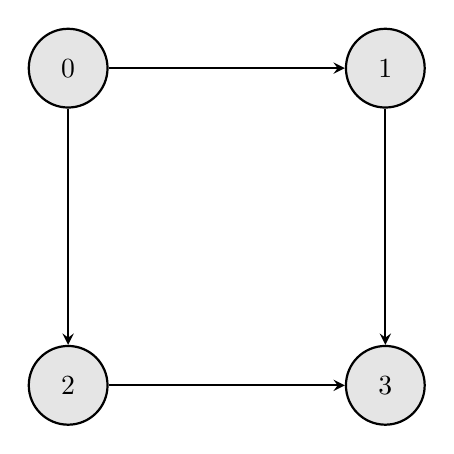
\begin{tikzpicture}
[every node/.style={draw, circle, fill=gray!20!, minimum size=1cm},
%level 1/.style={sibling distance=25mm},
%level 2/.style={sibling distance=15mm},
thick, >=stealth, ->]
\node(0){0};
\node(1)[right=3cm of 0]{1};
\node(2)[below=3cm of 0]{2};
\node(3)[right=3cm of 2]{3};
\draw (0) -- (1);
\draw (0) -- (2);
\draw (2) -- (3);
\draw (1) -- (3);
\end{tikzpicture}
\end{figure}

There are two paths: \fcj{0 -> 1 -> 3} and \fcj{0 -> 2 -> 3}.
\end{flushleft}

\paragraph{Note:}

\begin{itemize}
\item The number of nodes in the graph will be in the range \fcj{[2, 15]}.
\item You can print different paths in any order, but you should keep the order of nodes inside one path.
\end{itemize}

\subsection{DFS}
This is a typical \textbf{DFS} algorithm.

\setcounter{lstlisting}{0}
\begin{lstlisting}[style=customc, caption={DFS}]
vector<vector<int>> allPathsSourceTarget( vector<vector<int>>& graph )
{
    vector<vector<int>> ans;
    vector<int> path{0};
    auto len_g( static_cast< int >( graph.size() ) );
    dfs( 0, len_g - 1, graph, path, ans );
    return ans;
}
void dfs( int start, int dst, vector<vector<int>>& G, vector<int>& path, vector<vector<int>>& ans )
{
    if( start == dst )
    {
        ans.emplace_back( begin( path ), end( path ) );
        return;
    }
    for( int next : G[start] )
    {
        path.push_back( next );
        dfs( next, dst, G, path, ans );
        path.pop_back();
    }
}
\end{lstlisting}


\section{798 --- Smallest Rotation with Highest Score}

\textbf{Hard}

Given an array $A$, we may rotate it by a non-negative integer $K$ so that the array becomes $ A[K] $, $ A[K+1] $, $ A[K+2] $, $\ldots$, $ A[\lvert A\rvert - 1] $, $ A[0] $, $ A[1] $, $\ldots$, $ A[K-1] $.  Afterward, any entries that are less than or equal to their index are worth 1 point. 

For example, if we have \fcj{[2, 4, 1, 3, 0]}, and we rotate by $ K = 2 $, it becomes \fcj{[1, 3, 0, 2, 4]}.  This is worth 3 points because 

$ 1 > 0 $ [no points], 

$ 3 > 1 $ [no points], 

$ 0 \leq 2 $ [one point], 

$ 2 \leq 3 $ [one point], 

$ 4 \leq 4 $ [one point].

Over all possible rotations, return the rotation index $ K $ that corresponds to the highest score we could receive.  If there are multiple answers, return the smallest such index $ K $.
\paragraph{Example 1:}

\begin{flushleft}
\textbf{Input}: \fcj{[2, 3, 1, 4, 0]}

\textbf{Output}: 3

\textbf{Explanation}:  

Scores for each K are listed below: 

\fcj{K = 0},  \fcj{A = [2,3,1,4,0]}, score 2

\fcj{K = 1},  \fcj{A = [3,1,4,0,2]}, score 3

\fcj{K = 2},  \fcj{A = [1,4,0,2,3]}, score 3

\fcj{K = 3},  \fcj{A = [4,0,2,3,1]}, score 4

\fcj{K = 4},  \fcj{A = [0,2,3,1,4]}, score 3

So we should choose $ K = 3 $, which has the highest score.


\end{flushleft}
 

\paragraph{Example 2:}
\begin{flushleft}

\textbf{Input}: \fcj{[1, 3, 0, 2, 4]}

\textbf{Output}: 0

\textbf{Explanation}:  

$A$ will always have 3 points no matter how it shifts. So we will choose the smallest K, which is 0.


\end{flushleft}


\paragraph{Note:}

\begin{itemize}
\item $A$ will have length at most 20000.
\item $A[i]$ will be in the range \fcj{[0, A.length]}.
\end{itemize}

\subsection{Find Score Of Each Possible Position}
Suppose $N$ is the length of $A$. 

When $A[i]=0$, since any index is no less than zero, we can get score by putting $A[i]$ at any place. Conversely, if $A[i]=N$, we cannot get score from this number at any place. Thus, the range of numbers can score is $[1, N-1]$.

$(i-A[i]+N)\bmod N)$ is the value of $ K $ making $ A[i] $'s index just equal to $ A[i] $.

For example, If $ A[6] = 1 $, then $ K = (6 - A[6]) \bmod 6 = 5 $ making $ A[6] $ to index 1 of new array. Then if $K$ is bigger, i.e., $ K = (i - A[i] + 1) \bmod N $, we start to lose this point, and decrements the score.


Thus we can record the value of $K$ for all $ A[i] $ where we lose points.

\setcounter{lstlisting}{0}
\begin{lstlisting}[style=customc, caption={One Pass}]
int bestRotation( vector<int>& A )
{
    vector<int> bad( A.size(), 0 );
    auto N( static_cast<int>( A.size() ) );
    for( int i = 0; i < N; ++i )
    {
        //record the count of numbers
        //at index i - A[i] + N + 1
        //At this index, we will lost score
        bad[( i - A[i] + N + 1 ) % N] -= 1;
    }
	//find the position that we have maximum
	//count of nubmers.
    auto max_index( 0 );
    for( int i = 1; i < N; ++i )
    {
        bad[i] += bad[i - 1] + 1;
        if( bad[i] > bad[max_index] )
        {
            max_index = i;
        }
    }
    return max_index;
}
\end{lstlisting}
\section{799 --- Champagne Tower}

\textbf{Medium}

We stack glasses in a pyramid, where the first row has 1 glass, the second row has 2 glasses, and so on until the 100th row.  Each glass holds one cup (250ml) of champagne.

Then, some champagne is poured in the first glass at the top.  When the top most glass is full, any excess liquid poured will fall equally to the glass immediately to the left and right of it.  When those glasses become full, any excess champagne will fall equally to the left and right of those glasses, and so on.  (A glass at the bottom row has it's excess champagne fall on the floor.)

For example, after one cup of champagne is poured, the top most glass is full.  After two cups of champagne are poured, the two glasses on the second row are half full.  After three cups of champagne are poured, those two cups become full --- there are 3 full glasses total now.  After four cups of champagne are poured, the third row has the middle glass half full, and the two outside glasses are a quarter full.


Now after pouring some non-negative integer cups of champagne, return how full the $ j $-th glass in the $ i $-th row is (both $ i $ and $ j $ are 0 indexed.)

\paragraph{Example 1:}

\begin{flushleft}
\textbf{Input}: \fcj{poured = 1}, \fcj{query_glass = 1}, \fcj{query_row = 1}

\textbf{Output}: 0.0

\textbf{Explanation}: 

We poured 1 cup of champange to the top glass of the tower (which is indexed as (0, 0)). There will be no excess liquid so all the glasses under the top glass will remain empty.
\end{flushleft}

\paragraph{Example 2:}

\begin{flushleft}
\textbf{Input}: \fcj{poured = 2}, \fcj{query_glass = 1}, \fcj{query_row = 1}

\textbf{Output}: 0.5

\textbf{Explanation}: 

We poured 2 cups of champange to the top glass of the tower (which is indexed as \fcj{(0, 0)}). There is one cup of excess liquid. The glass indexed as \fcj{(1, 0)} and the glass indexed as \fcj{(1, 1)} will share the excess liquid equally, and each will get half cup of champange.
\end{flushleft}
 

\paragraph{Note:}

\begin{flushleft}
\item \fcj{poured} will be in the range of $ [0, 10 ^ 9] $.
\item \fcj{query_glass} and \fcj{query_row} will be in the range of \fcj{[0, 99]}.
\end{flushleft}

\subsection{Dynamic Programming}
Instead of keeping track of how much champagne should end up in a glass, keep track of the total amount of champagne that flows through a glass. For example, if \fcj{poured = 10} cups are poured at the top, the total flow-through of the top glass is 10; the total flow-through of each glass in the second row is 4.5, and so on.

We use $F[i][j]$ as the amount of champagne at $i$-th row and $j$-th glass. At start $F[0][0]$ is the total poured champagne. Then we split the excess amount of champagne into next level's glasses.

Since we have to compute the next row after \fcj{query_row}, the size of the $F$ is will be \fcj{(query_row+2, query_row+2)}

\setcounter{lstlisting}{0}
\begin{lstlisting}[style=customc, caption={Simulation}]
double champagneTower( int poured, int query_row, int query_glass )
{
    vector<vector<double>> F( query_row + 2, vector<double>( query_row + 2, 0. ) );
    //at start, we have poured amount of champagne at the top
    F[0][0] = poured;
    for( int i = 0; i <= query_row; ++i )
    {
        //simulate water flow from 0 to i
        for( auto j( 0 ); j <= i; ++j )
        {
            if( F[i][j] > 1 )
            {
                //(i+1,j) and (i+1,j+1) are the
                //glasses that champagne will flow from (i,j)
                F[i + 1][j] += ( F[i][j] - 1 ) / 2.0;
                F[i + 1][j + 1] += ( F[i][j] - 1 ) / 2.0;
            }
        }
    }
    return ( min )( 1.0, F[query_row][query_glass] );
}
\end{lstlisting}
\end{document}
